% IAMAS Master's Thesis LaTeX Format ver.1.0 - English Version

% For uplatex compilation (supports UTF-8 special characters)
\documentclass[uplatex,dvipdfmx]{ujarticle}
% For platex compilation, comment above and uncomment below:
%\documentclass[dvipdfmx]{jsarticle}

\usepackage[top=25truemm,bottom=30truemm,left=30truemm,right=30truemm]{geometry}

\usepackage{iamas}
\usepackage{amsmath}
\usepackage[dvipdfmx]{graphicx}
\usepackage{plext}
\usepackage{ascmac}
\usepackage{url}
\usepackage{wrapfig}
\usepackage{setspace}
\usepackage{chicago}
\usepackage{afterpage}
\usepackage{here}
\usepackage{caption}

% Multi-language support packages
\usepackage{otf}
\usepackage[T1]{fontenc}
\usepackage[utf8]{inputenc}
\usepackage[prefernoncjk]{pxcjkcat}

\begin{document}

% Include sections
% Title page
\title{\Large Attempt to Create Music with Multilayered Temporal Structures and Possibility of Embodiment for Player and Audience}
\author{Hiroshi YAMATO}
\date{\today}

\maketitle
\large

% Note: The Japanese abstract tables are included as PDF figures in the original
% The English abstract is already provided in the original document
% For the purpose of this translation, we will include the abstract figures as-is

\begin{figure}[ht]
\centerline{
	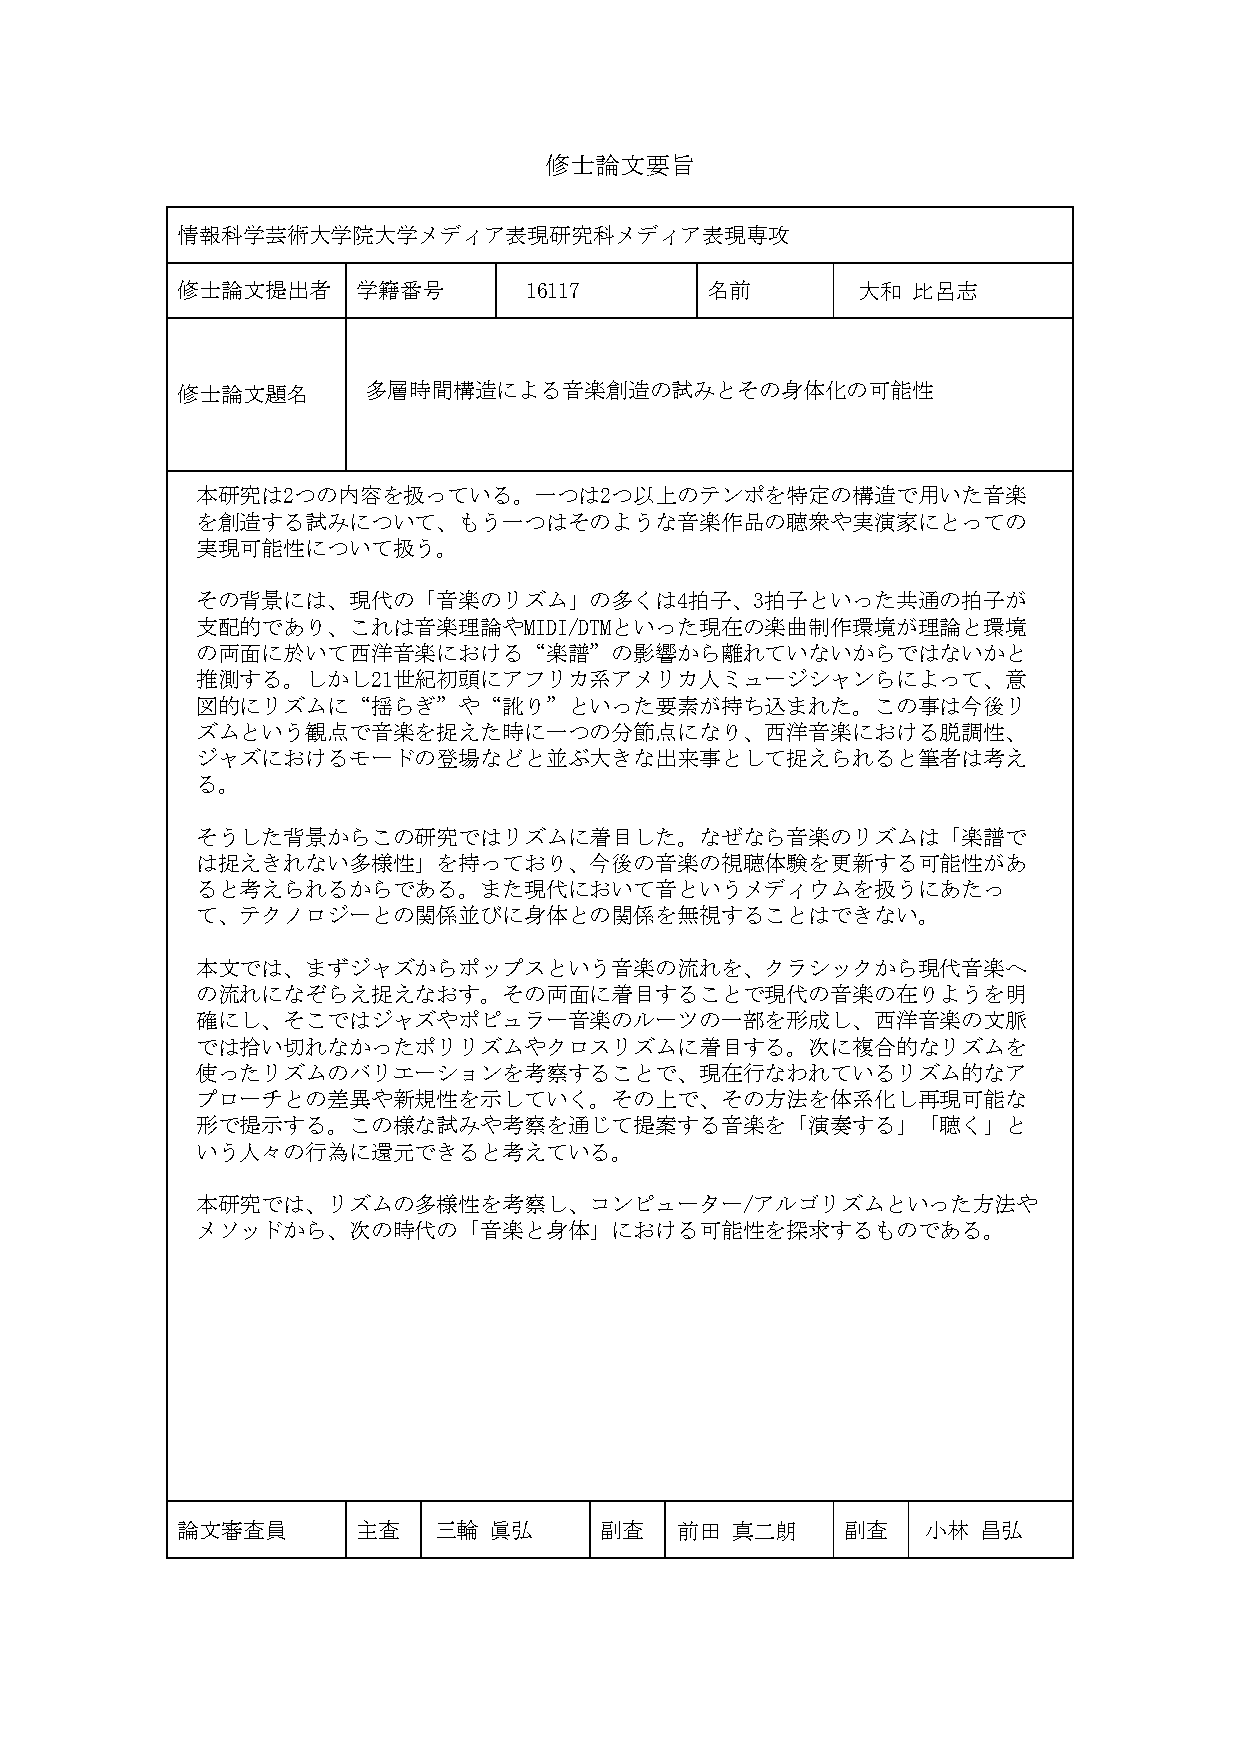
\includegraphics[
 width=\textwidth]{./PDF/abstract_jp.pdf}
}
\end{figure}

\begin{figure}[ht]
\centerline{
	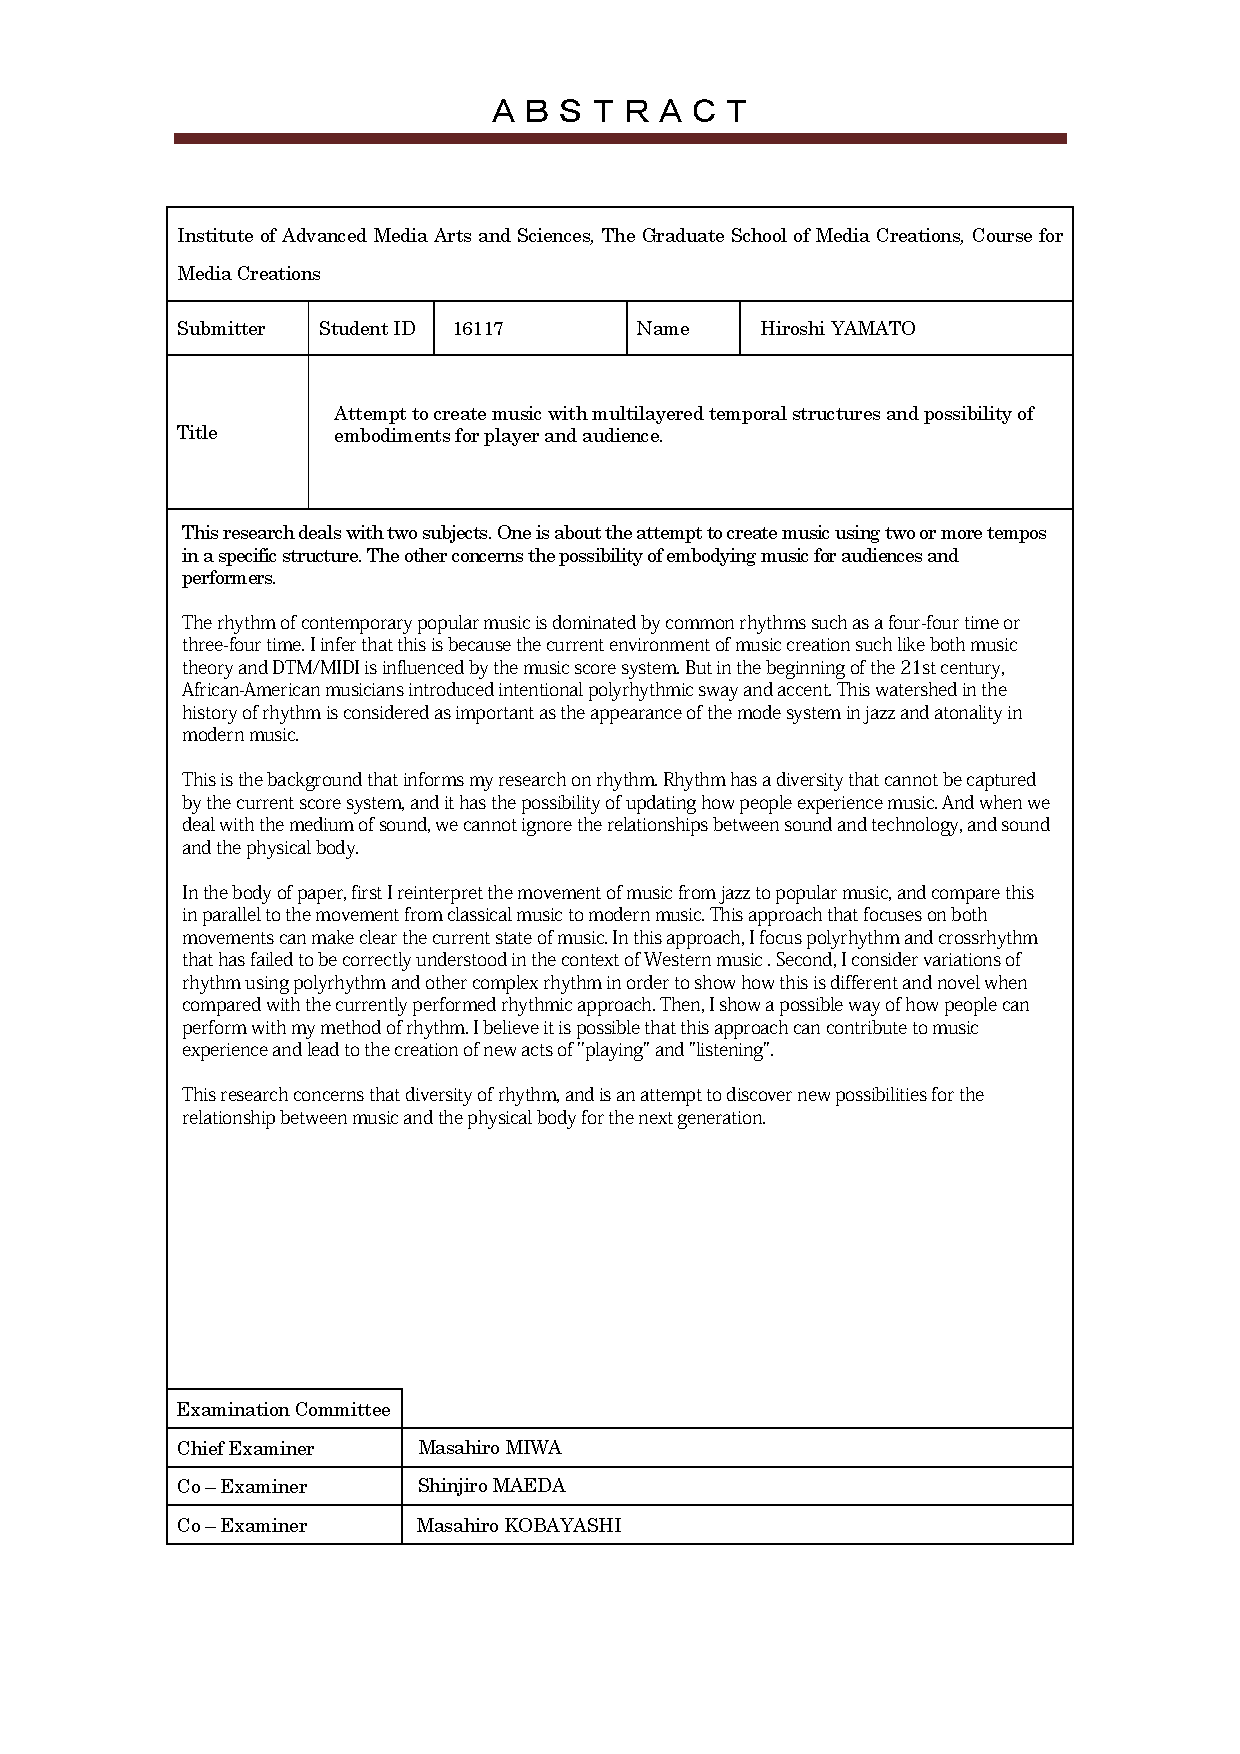
\includegraphics[
 width=\textwidth]{./PDF/abstract_en.pdf}
}
\end{figure}

% Page break for proper formatting
\afterpage{\clearpage}
\newpage

% Table of contents
\tableofcontents

\afterpage{\clearpage}
\newpage

% Main content
\section{Introduction}
When considering the 100 years of the 20th century in popular music including jazz, it can be said that ``{\bf the 20th century was a hundred years in which music born in the southern United States spread around the world in various forms}''\cite{murai:01}. It goes without saying that this development began with sheet music in the early days and was disseminated through the invention of radio, records, and mass media. However, why is there a predominance of common time signatures such as 4/4 or 3/4 in much of this music's rhythm? The author believes that even in modern times, the system for describing music—``the musical score as a protocol connecting composers and performers''—inherited from classical music has a strong influence on music theory such as the Berklee Method and modern music production environments.

On the other hand, many attempts have been made to depart from existing rhythmic forms in contemporary music, free jazz, noise music, and electronica. However, most of these have been included as partial elements in modern popular music without changing or updating the rhythmic forms themselves.

Therefore, focusing on approaches to jazz rhythm in the modern era from around the 21st century, such as ``polyrhythm/cross-rhythm characteristics'' and ``fluctuations and inflections in rhythm,'' and expanding these methods as a critical attempt toward 20th-century music, the author devised ``music with multilayered temporal structures.'' As a practical example, a series of works titled ''{\bf Music for multilayered temporal structures}''\cite{yamato:01} was composed, and performances by jazz musicians were attempted and recorded to examine whether actual performance was possible.

\subsection{Scope of This Research \label{research_target}}
As stated in the introduction, this research presents a critical perspective on the rhythmic forms of current popular music, as well as production environments such as notation and DTM, from the viewpoint of ``possibilities for future rhythmic approaches.'' Regarding why such a critical attempt is necessary, Yuval Noah Harari states in \textit{Sapiens: A Brief History of Humankind}:\\

{\bf Just as medieval culture could not reconcile chivalry with Christianity, so the modern world fails to reconcile liberty with equality. But this is no defect. Such contradictions are an inseparable part of every human culture. In fact, they are culture's engines, responsible for the creativity and dynamism of our species. Just as when two clashing musical notes played together force a piece of music forward, so discord in our thoughts, ideas and values compels us to think, reevaluate and criticize. Consistency is the playground of dull minds.
If tensions, conflicts, and irresolvable dilemmas are the spice of every culture, a human being who belongs to any particular culture must hold contradictory beliefs and be riven by incompatible values. It's such an essential feature of any culture that it even has a name: cognitive dissonance. Cognitive dissonance is often considered a failure of the human psyche. In fact, it is a vital asset. Had people been unable to hold contradictory beliefs and values, it would probably have been impossible to establish and maintain any human culture.} \cite{harari:01}\\

The ``dissonance'' that Harari mentions here is clearly not musical dissonance but a metaphor. However, as shown in Figure \ref{fig:figure_08}\cite{murai:01}, the collision between African music and Irish music of Islamic origin within Creole culture, which became one of the origins of jazz and had a major influence on today's popular music and was also the impetus for the birth of blues music, can also be described as the ``cognitive dissonance for humanity to establish culture'' that Harari refers to. It can also be considered that such cognitive dissonance has occurred in various forms to this day, maintaining and developing culture as popular music.

\begin{figure}[ht]
\centerline{
	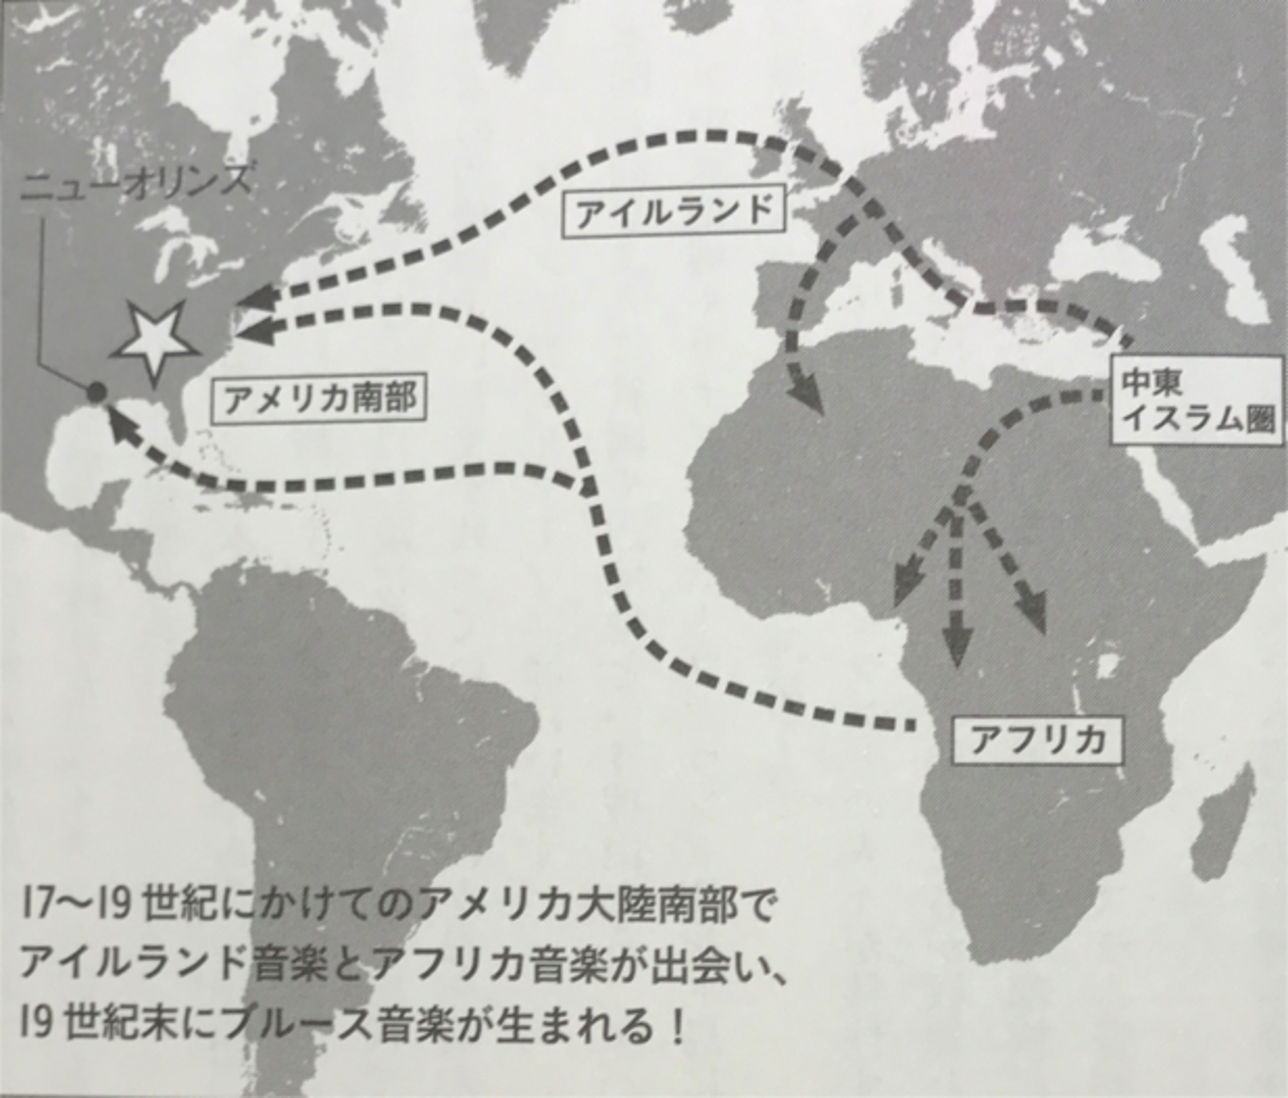
\includegraphics[
 width=0.5\textwidth]{./PDF/figure_08.pdf}
}
\caption{Mukai Yasushi (\textit{Jazz History That Changes Your Listening}, p17, 2017)\\
A diagram showing the origin of blues, where music from the Middle Eastern Islamic region influenced and passed through African music and Irish music, then converged in the southern United States}
\label{fig:figure_08}
\end{figure}

Furthermore, the purpose of this research is to carry out the movement from dissonance to harmony that Harari describes through ``approaches to rhythm,'' prompting listeners, performers, and composers to reevaluate, criticize, and critique, thereby creating ``cognitive dissonance through rhythm'' and contributing to advancing music as a culture.

To this end, this research and the works produced in the process will be discussed primarily within the context of popular music. Specifically, through the development of the Berklee Method, which formed the foundation of popular music, and the creation of jazz-based works using lead sheet notation, which is one of the reasons for the worldwide spread of this theory, this research will address approaches to rhythm, notation methods, and performance feasibility.


\subsection{Similarities Between Modern Popular Music History and Western Music History}

This research examines so-called ``popular music,'' and its background will be discussed here. First, when proceeding with the argument on the two axes of ``Western music'' and ``popular music'' in this section, each will be defined as follows.

\begin{description}
 \item[Western music]\mbox{}\\
	    Refers mainly to classical music and contemporary music before the 20th century. Also includes music from the 20th century onward that follows this style.
 \item[Popular music]\mbox{}\\
	    Refers mainly to music based on blues and jazz as American ethnic music from the 20th century onward. Includes commercial music in general.
\end{description}

As the basis for such a division, Peter van der Merwe states in \textit{Origins of the Popular Style}: ``{\bf By the time the first blues was published, all the materials available to twentieth-century popular music composers were in place. Since then, popular music has incorporated various ethnic styles, drawn inspiration from classical music, and combined the styles at hand in every possible way. (omitted) But fundamentally speaking, no elements have been created whose origins do not date back to before the 1900s}'' \cite{merwe:01}. However, at the same time, Merwe also states: ``{\bf The term `popular music' is a label, not a content. (omitted) Being popular, whether it means `favored by the people' or `of the masses,' is only a temporary value}'' \cite{merwe:01}. This indicates that the two definitions divided above are merely a convenient division based on historical background and do not indicate their value.

Assuming such a division is possible, what is important here is Merwe's earlier observation that ``no elements have been created whose origins do not date back to before the 1900s.'' This demonstrates the self-evidence that ``popular music'' contains within it the context of ``Western music,'' but the author attempts to present both the similarities and what ``Western music'' has overlooked, as well as the present state of ``popular music,'' by placing ``Western music'' and ``popular music'' in parallel based on their developmental history.

First, when considering ``Western music'' as the flow from so-called ``classical music to contemporary music (including American New Music such as John Cage and Steve Reich),'' we can broadly understand it as the establishment of tonality in the Baroque period from the 17th to 18th centuries, the Romantic period and popularization from opera to aria in the 19th century, and the flow to contemporary music through the expansion of tonality from twelve-tone technique and serialism in the 20th century. When comparing ``popular music'' with the flow toward blues and jazz as American ethnic music, the diversification and theorization of styles such as the ``popular music theory'' born there—the Berklee Method, modal jazz, and free jazz—followed by mass production and media distribution and development of pop music leading to popularization, and the expansion of diversity through electronics, both can be seen to follow a flow of ``establishment of tonality, expansion, and atonality.'' In particular, the chord system spread by the Berklee Method after entering the 20th century and the high analytical nature of that system greatly changed the production field from before its appearance, and it can be said that ``{\bf the Berklee Method represents the first peak of symbolization in the history of `commercial music,' probably in a history that will continue for a long time to come}'' \cite{kikuchi-ootani:01}. This can also be described as ``{\bf symbolization = commercialization = emphasis on phonemes}'' \cite{kikuchi-ootani:01}, similar to the flow of ``establishment of tonality to popularization'' in Western music. Also, if we place the movement from ``expansion of tonality to contemporary music'' in ``Western music'' in parallel with ``mode, free, noise as methods, and the development and diversity of technology/electronics'' in ``popular music,'' both can be understood as a movement of ``expansion of tonality to atonality.'' By understanding both in parallel in this way, it can be said that much of the flow of ``establishment of system,'' ``expansion of system,'' and ``departure from system'' is being carried out by both centered on ``tonality.'' Furthermore, by understanding modern ``popular music'' from this standpoint, it becomes possible to consider the possibilities of future music.


\section{What are Polyrhythm and Cross-rhythm?}

In the \textit{New Music Dictionary} (40th edition, 1996) published by Ongaku no Tomo Sha, "polyrhythm" is defined as "\textbf{a phenomenon in which contrasting rhythms are used simultaneously in two or more voices, also called cross-rhythm}"\cite{asaka:01}. The dictionary also cites the opening of J.S. Bach's "Sinfonia No. 9" as an example, noting that "\textbf{it is generally distinguished from the rhythmic symmetry that promotes the independence of voices inherent to polyphony}"\cite{asaka:01}. However, this suggests that even today, the definition of "polyrhythm/cross-rhythm" has not been established in a definitive manner. Furthermore, Yoda and Ono point out in their \textit{Music Theoretical Analysis of Polyrhythm Typology} that "\textbf{even by consulting only three music dictionaries, it becomes clear that the definition of polyrhythm is extremely diverse and ambiguous. Rhythm research has been historically neglected compared to harmony and other elements}"\cite{yoda-ono:01}, and they attempt to present a typology of polyrhythms. The fact that rhythm research has not been given as much weight as harmony can also be understood from Jean-Yves Bosseur's \textit{88 Keywords to Understanding Contemporary Music}, where most of the techniques discussed concern phonology, temperament, and acoustics, even in contemporary music. However, while the typology conducted by Yoda and Ono provides detailed analysis, it is classified using Western musical terminology that is not common in contemporary popular music. Here, separately from Yoda and Ono's analysis, we will examine "polyrhythm/cross-rhythm" in light of contemporary "popular music" situations, referring to "African polyrhythm" as the foundation for definition, and addressing "polyrhythm/cross-rhythm" as something that "Western music" has overlooked and as the present state of "popular music."

In this paper, we will explain the definition of polyrhythm based on African rhythms as "non-Western music," establish our definition of "polyrhythm/cross-rhythm," and then examine the "polyrhythmic/cross-rhythmic" nature of rhythms from Indian, Middle Eastern, and Latin genres. Subsequently, we will similarly examine "Western music" and "popular music," and finally consider the current state of "Western music" and "popular music" with regard to rhythm.

\subsection{Polyrhythm/Cross-rhythm in Non-Western Music}
\subsubsection{Africa}

Kikuchi and Otani state that "\textbf{one cycle of 12 is the prototype of polyrhythm in African music}"\cite{kikuchi-ootani:01} and that "\textbf{the basic polyrhythm of Africa is a cross between 4-beat and 3-beat time}"\cite{kikuchi-ootani:01}. This tendency can be affirmed from Tsukada's discussion of Brandel's vertical hemiola in \textit{The Truth About African Music} and from "the relationship between rhythm patterns (standard rhythm patterns) and beats coexisting in Africa"\cite{tsukada:01}.

Regarding Brandel's vertical hemiola, Tsukada states the following: "\textbf{Let us focus on the relationship between the song and hand claps in 'Song at Sunset' (Figure \ref{fig:figure_14}). The hand claps consistently proceed in 6/8 time, that is, in 2-division, so in the sections where the melody proceeds in 3/4 time (measures 1, 2, 5, and 7), rhythm patterns of 2-division and 3-division are simultaneously combined}"\cite{tsukada:01}. This is what Brandel calls vertical hemiola. Tsukada also describes this vertical hemiola as "\textbf{the most primitive form of African polyrhythm}"\cite{tsukada:01}. Furthermore, he states that "\textbf{if we consider that the complex polyrhythms of Africa are a highly developed form of this prototypical rhythm structure, then this vertical hemiola is precisely the characteristic African rhythm structure that Jones repeatedly emphasized in his polyrhythm theory, and the hand clap rhythm seen in 'Song at Sunset' is what Agawu calls 'the 6/8 time consistently present in the background of the piece'}"\cite{tsukada:01}, thus relating it to past polyrhythm research and demonstrating its validity.

\begin{figure}[ht]
\centerline{
	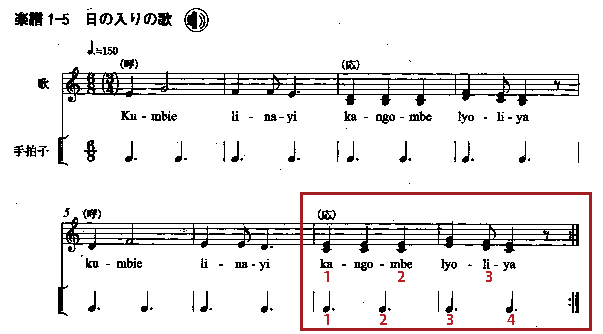
\includegraphics[
 width=\textwidth]{./PDF/figure_14.pdf}
}
\caption{Kenichi Tsukada (\textit{The Truth About African Music} p.41, Score 1-5, 2016)\\
In measures 1, 3, 5, and 7, the form of Brandel's vertical hemiola with 2-beat and 3-beat can be observed. Red frames and red text added by the author. The structure where "3-beat and 4-beat cross," as described by Kikuchi and Otani, can be seen.}
\label{fig:figure_14}
\end{figure}

The "prototype of African music polyrhythm" presented by Kikuchi and Otani can also be observed in Figure \ref{fig:figure_14} cited in Tsukada's discussion of vertical hemiola. Focusing on measures 7 and 8 enclosed in the red frame in Figure \ref{fig:figure_14}, and viewing these two measures as one unit of 12 beats, we can see that the hand claps are struck evenly four times. Furthermore, focusing on the quarter notes on beats 1 and 3 of measure 7 in the song, and the eighth note on beat 2 of measure 8, we can identify three evenly spaced strike points within the whole, confirming the same form with a 12-beat cycle: the song at 4+4+4, and the hand claps at 3+3+3+3 in eighth notes.

Regarding the 12-beat cycle rhythm pattern, "\textbf{as soon as one crosses the Sahara Desert from the north of the African continent, this rhythm pattern can suddenly be heard everywhere}"\cite{tsukada:01}, and its basic rhythm is summarized as shown in Figure \ref{fig:figure_15}. Furthermore, as shown in Figure \ref{fig:figure_16}, this basic rhythm is such that "\textbf{when Africans perform the standard rhythm pattern, they perform while feeling the eighth note as the 'basic pulse'}"\cite{tsukada:01}, and moreover, "\textbf{when performing the standard rhythm pattern, they feel three of these basic pulses as one unit (beat)}"\cite{tsukada:01}. From this, it can be considered that performances have been conducted in the form defined by Kikuchi and Otani.

\begin{figure}[ht]
\centerline{
	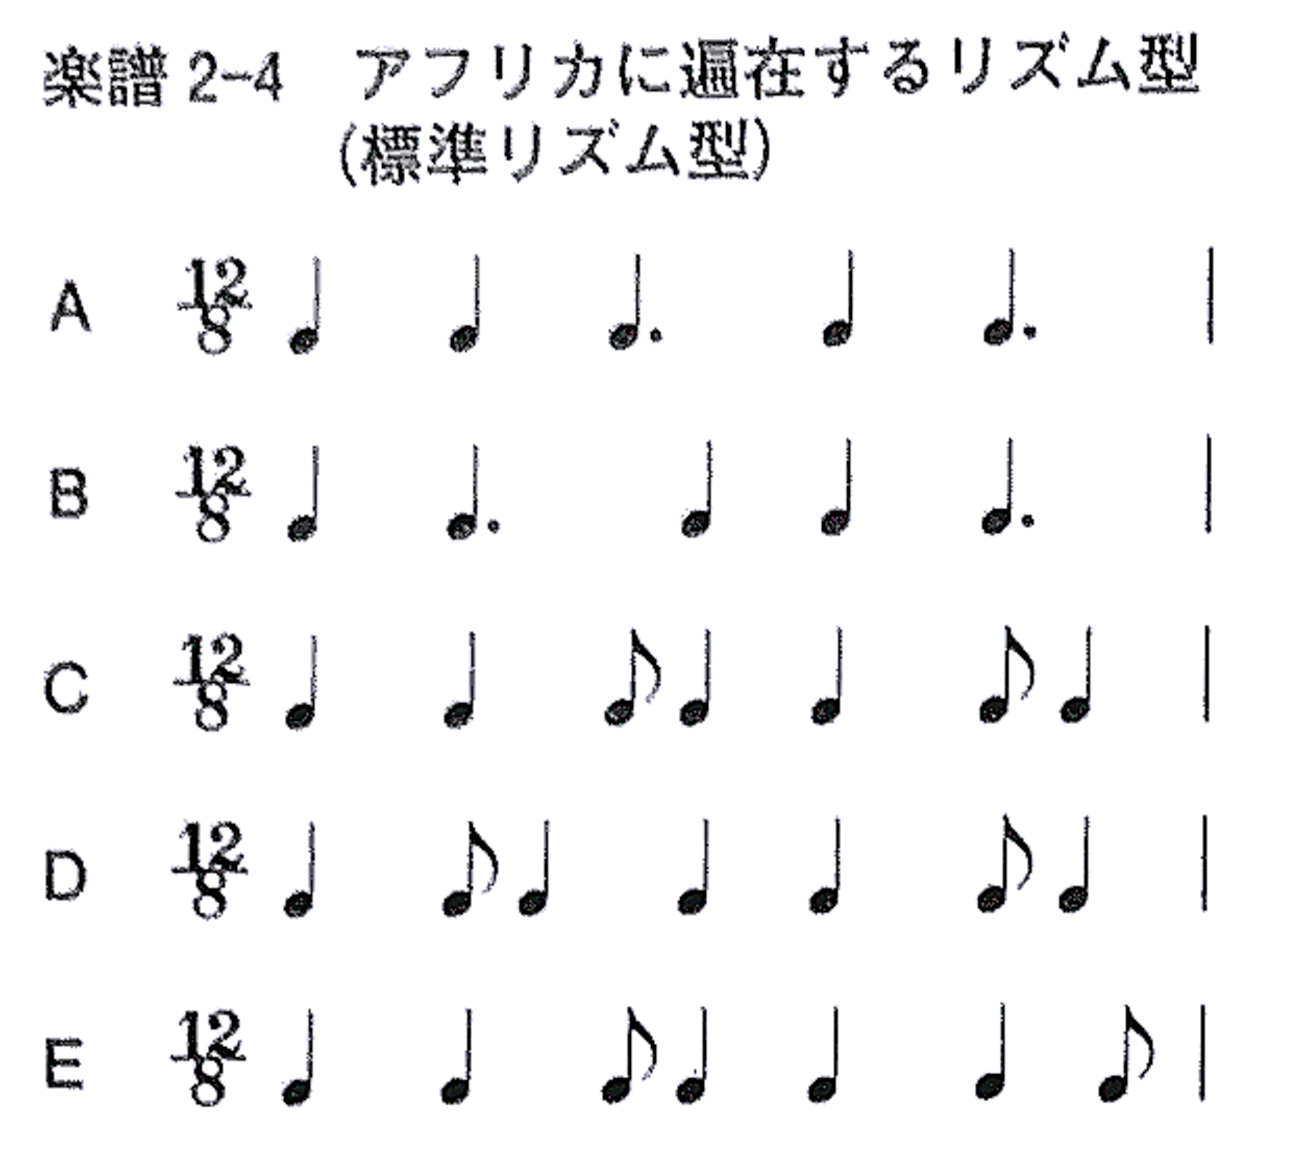
\includegraphics[
 width=0.5\textwidth]{./PDF/figure_15.pdf}
}
\caption{Kenichi Tsukada (\textit{The Truth About African Music} p.59, Score 2-4, 2016)}
\label{fig:figure_15}
\end{figure}

\begin{figure}[ht]
\centerline{
	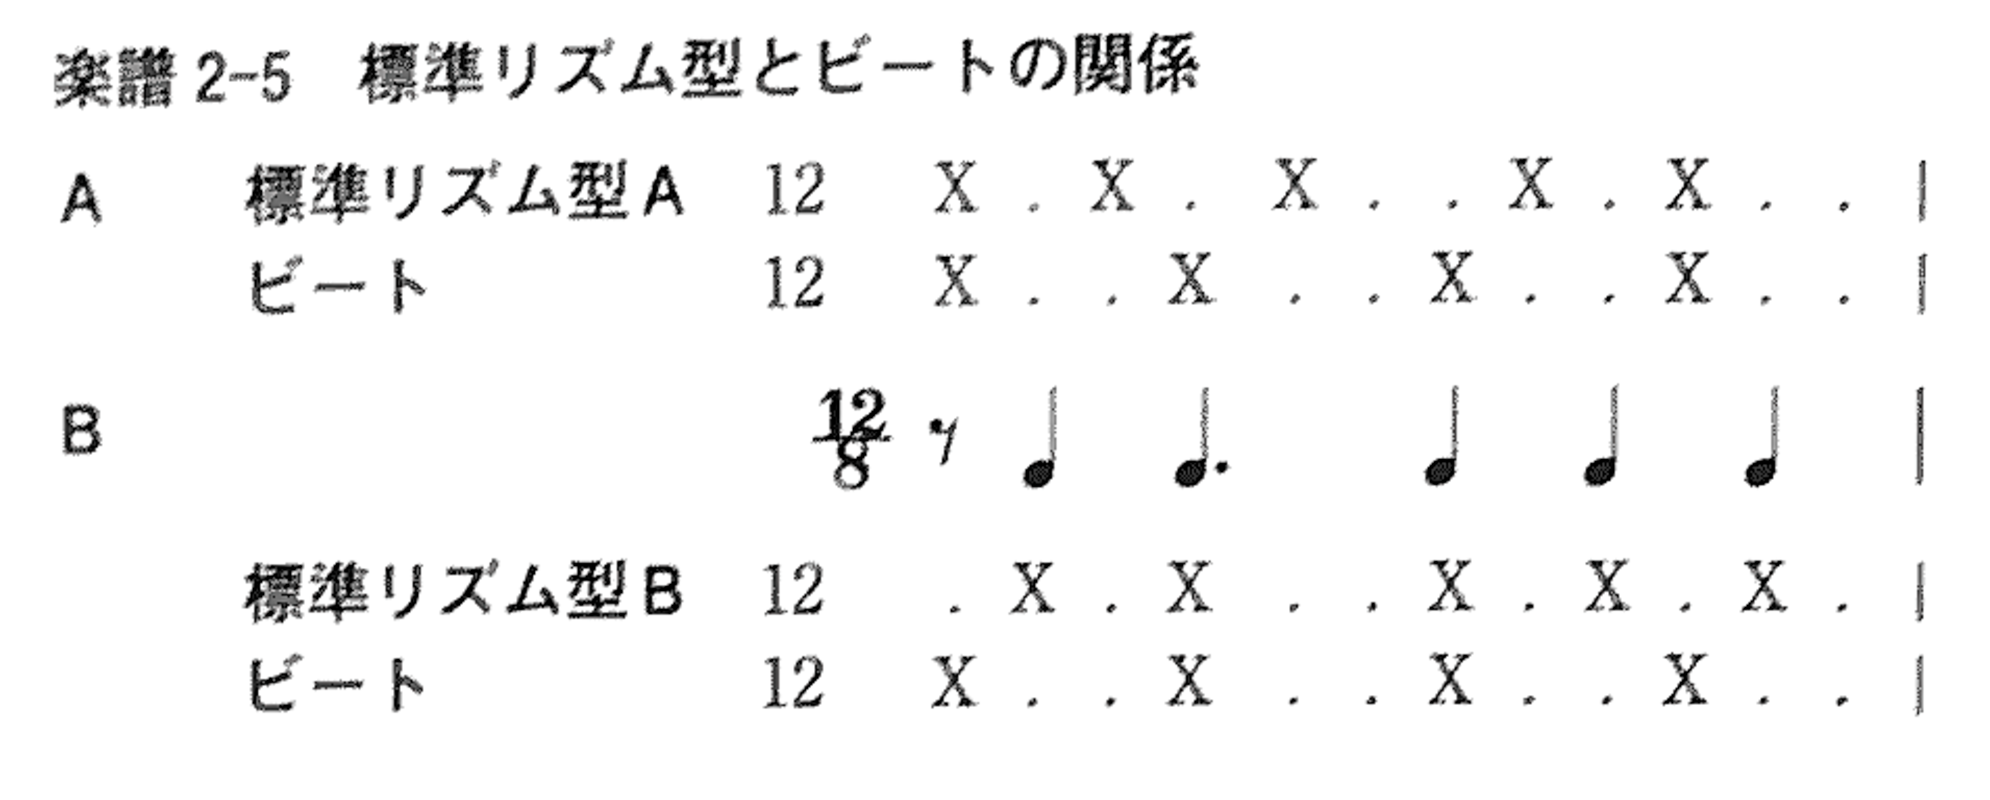
\includegraphics[
 width=0.75\textwidth]{./PDF/figure_16.pdf}
}
\caption{Kenichi Tsukada (\textit{The Truth About African Music} p.61, Score 2-5, 2016)}
\label{fig:figure_16}
\end{figure}

\subsubsection{Definition of Polyrhythm/Cross-rhythm}

As discussed above, the general interpretation of "polyrhythm" is broad, but when examining African polyrhythm, a certain structure can be identified. Regarding this structure, Kikuchi and Otani state: "\textbf{The cross-rhythm of 3 and 4 is, by my definition, no longer polyrhythm. That is African-style monorhythm (omitted). Only when you enter into the accents or the contraction of time sense that arises from it do you enter the African polyrhythmic stage (omitted). In today's commercial music, I would like to consider the 3 and 4 cross we just did as fundamental}"\cite{kikuchi-ootani:01}. Tsukada also points out, as an example of vertical hemiola appearing in commercial music, "\textbf{in the song 'Polyrhythm' (composed by Yasutaka Nakata) that the Japanese techno-pop unit Perfume hit in 2007, a powerful and impressive vertical hemiola structure appears in the interlude section}"\cite{tsukada:01}.

Therefore, "polyrhythm/cross-rhythm" in this thesis is defined as follows, based on Kikuchi and Otani's definition:

\begin{description}
 \item[Cross-rhythm]\mbox{}\\
	    Two or more time signatures that divide one cycle unit by integer ratios. Vertical hemiola-type rhythm.
 \item[Polyrhythm]\mbox{}\\
	    Two or more time signatures that do not divide one cycle unit by integer ratios. Rhythm with sway or accent.
\end{description}

According to this definition, the 12-beat cycle rhythm with 3-beat and 4-beat pulses, previously considered the basic African polyrhythm, has 12 as its least common multiple and is classified as cross-rhythm. A polyrhythmic state would be, in a simple example, a rhythm with 4-beat and 5-beat pulses against a 12-cycle: dividing 12 beats by 4 yields a beat unit of 3 beats, which divides evenly as an integer, but dividing by 5 results in a beat unit of 2.4 beats, which does not divide evenly.

Based on this definition, we will now examine the polyrhythmic/cross-rhythmic situations in India, the Middle East, and Latin music.

\subsubsection{India}

In Indian music, there exists a rhythmic form called tala, which "\textbf{takes the form of measures similar to Western music, but has created many types of time division arrangements}"\cite{deva:01}. Tala is "\textbf{defined as an arrangement with periodicity of a certain pattern}"\cite{deva:01}, and "\textbf{the essence of tala lies in its periodicity and repetitiveness}"\cite{deva:01}. Regarding the polyrhythmic/cross-rhythmic nature of Indian music using tala, Sachs indicates this in \textit{Rhythm and Tempo} with the terms "contrapuntal rhythm" and "overlap of two patterns."

First, regarding "contrapuntal rhythm," he states: "\textbf{Simple contrapuntal rhythm uses the same tala. That is, one hand plays the pattern at standard tempo, while the other hand expands its length}"\cite{sachs:01}. Figure \ref{fig:figure_17} illustrates this.

\begin{figure}[ht]
\centerline{
	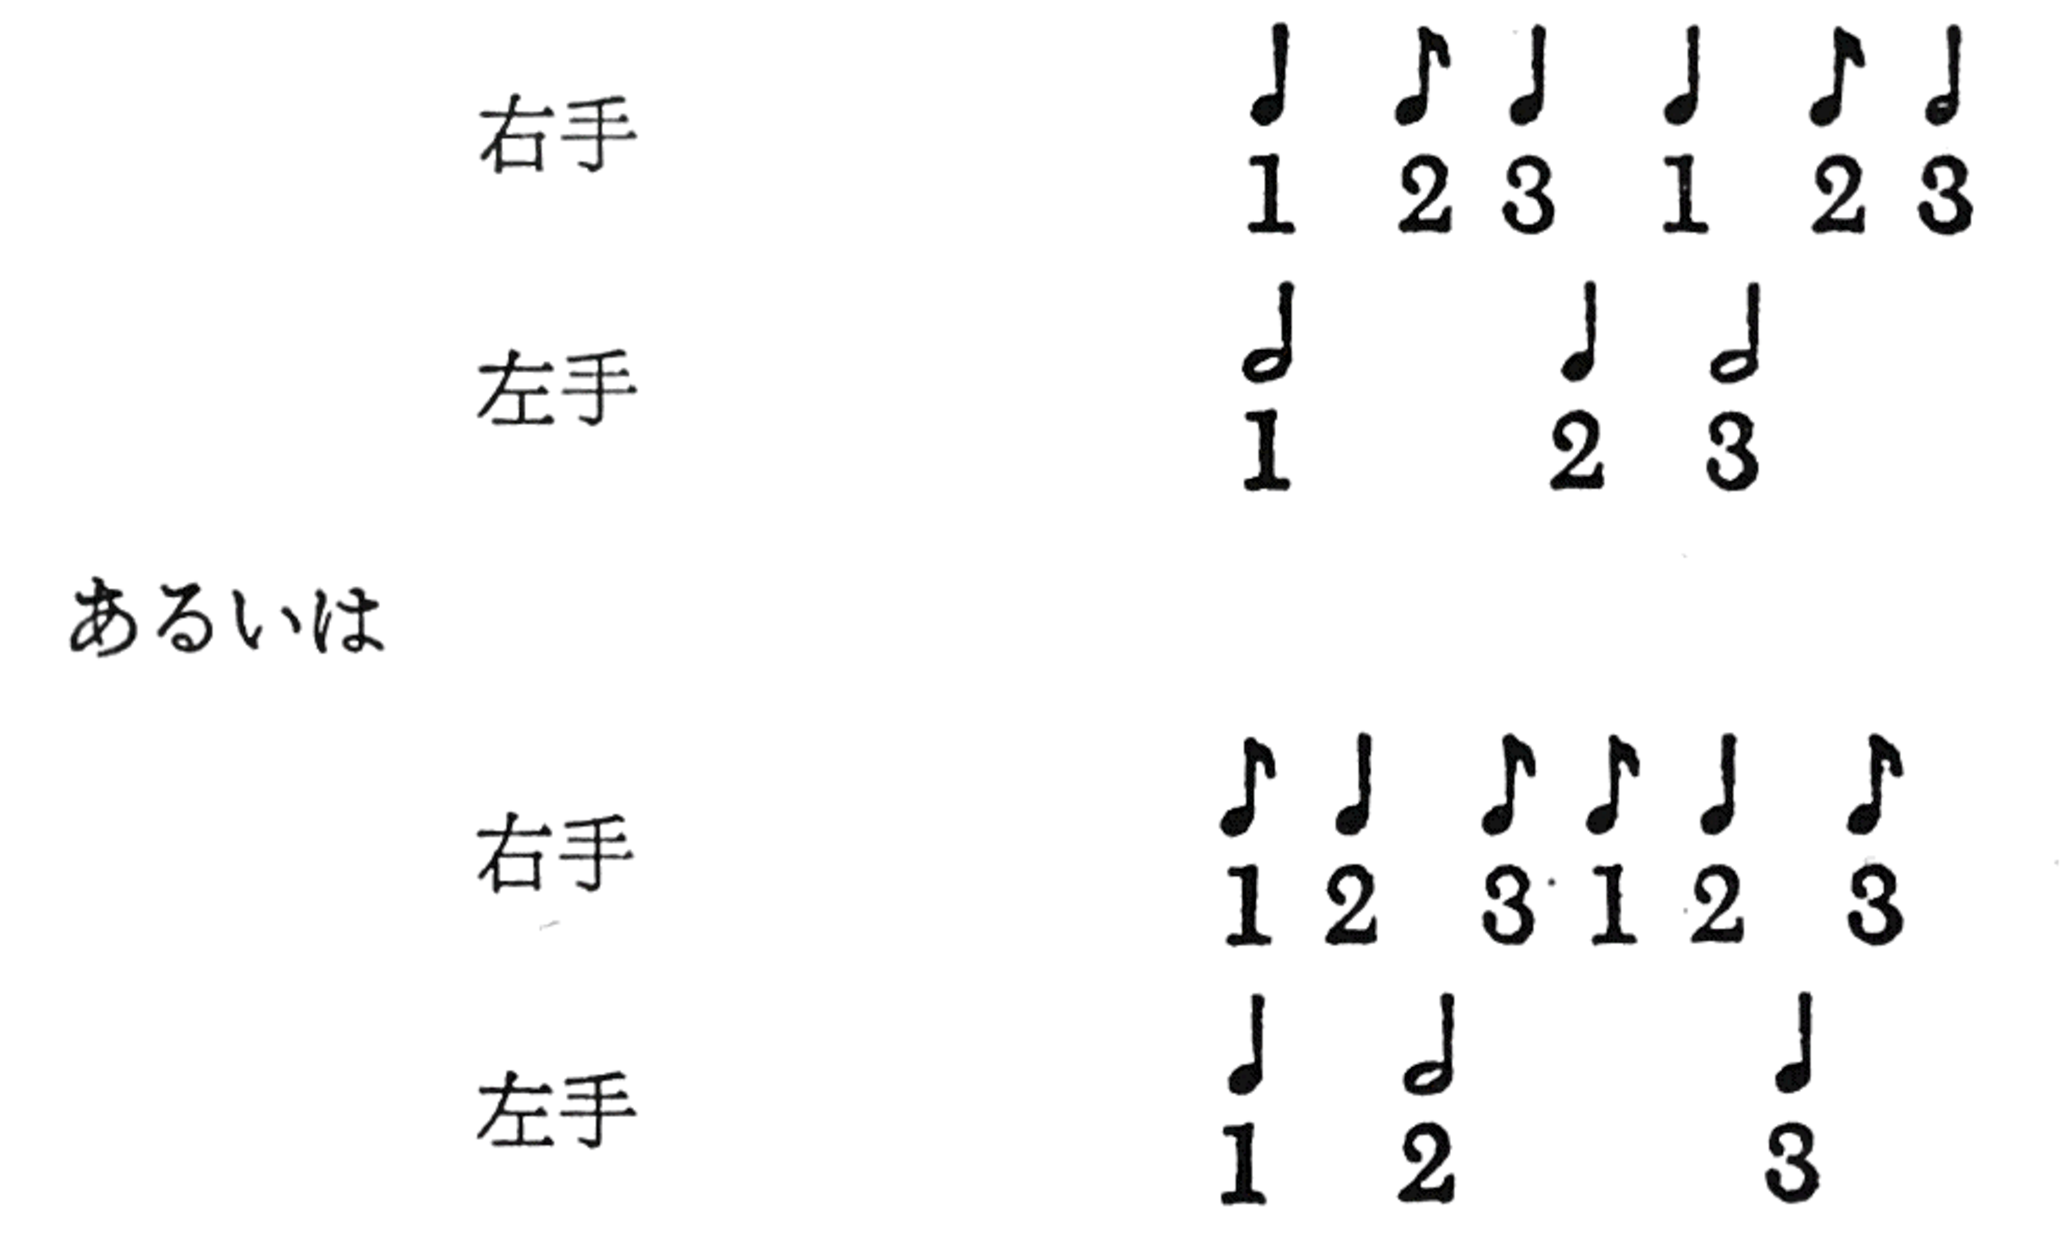
\includegraphics[
 width=0.5\textwidth]{./PDF/figure_17.pdf}
}
\caption{Curt Sachs (\textit{Rhythm and Tempo} p.106, 1979)\\
Example of oppositional rhythm. The left hand is expanded to twice the length of the right hand's rhythm.}
\label{fig:figure_17}
\end{figure}

As another example of "contrapuntal rhythm," he states: "\textbf{It frequently happens that both hands play different talas. As follows, one hand plays at standard tempo while the other hand plays at expanded tempo}"\cite{sachs:01}, showing this in Figure \ref{fig:figure_18}.

\begin{figure}[ht]
\centerline{
	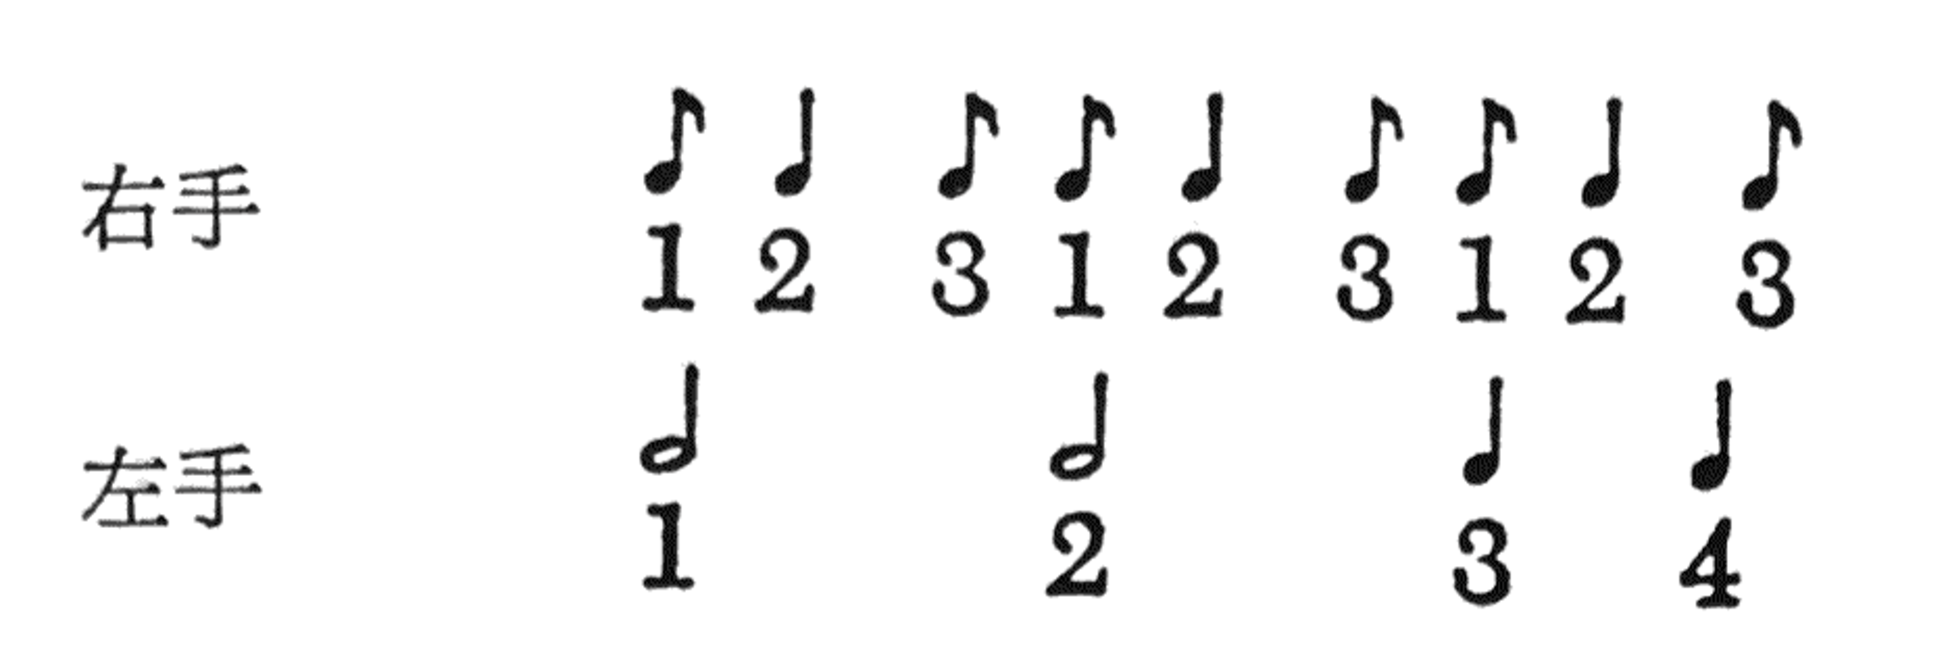
\includegraphics[
 width=0.5\textwidth]{./PDF/figure_18.pdf}
}
\caption{Curt Sachs (\textit{Rhythm and Tempo} p.107, 1979)\\
Example of performing different talas with right and left hands}
\label{fig:figure_18}
\end{figure}

As an example of "overlap of two patterns," he presents Figure \ref{fig:figure_19}.

\begin{figure}[ht]
\centerline{
	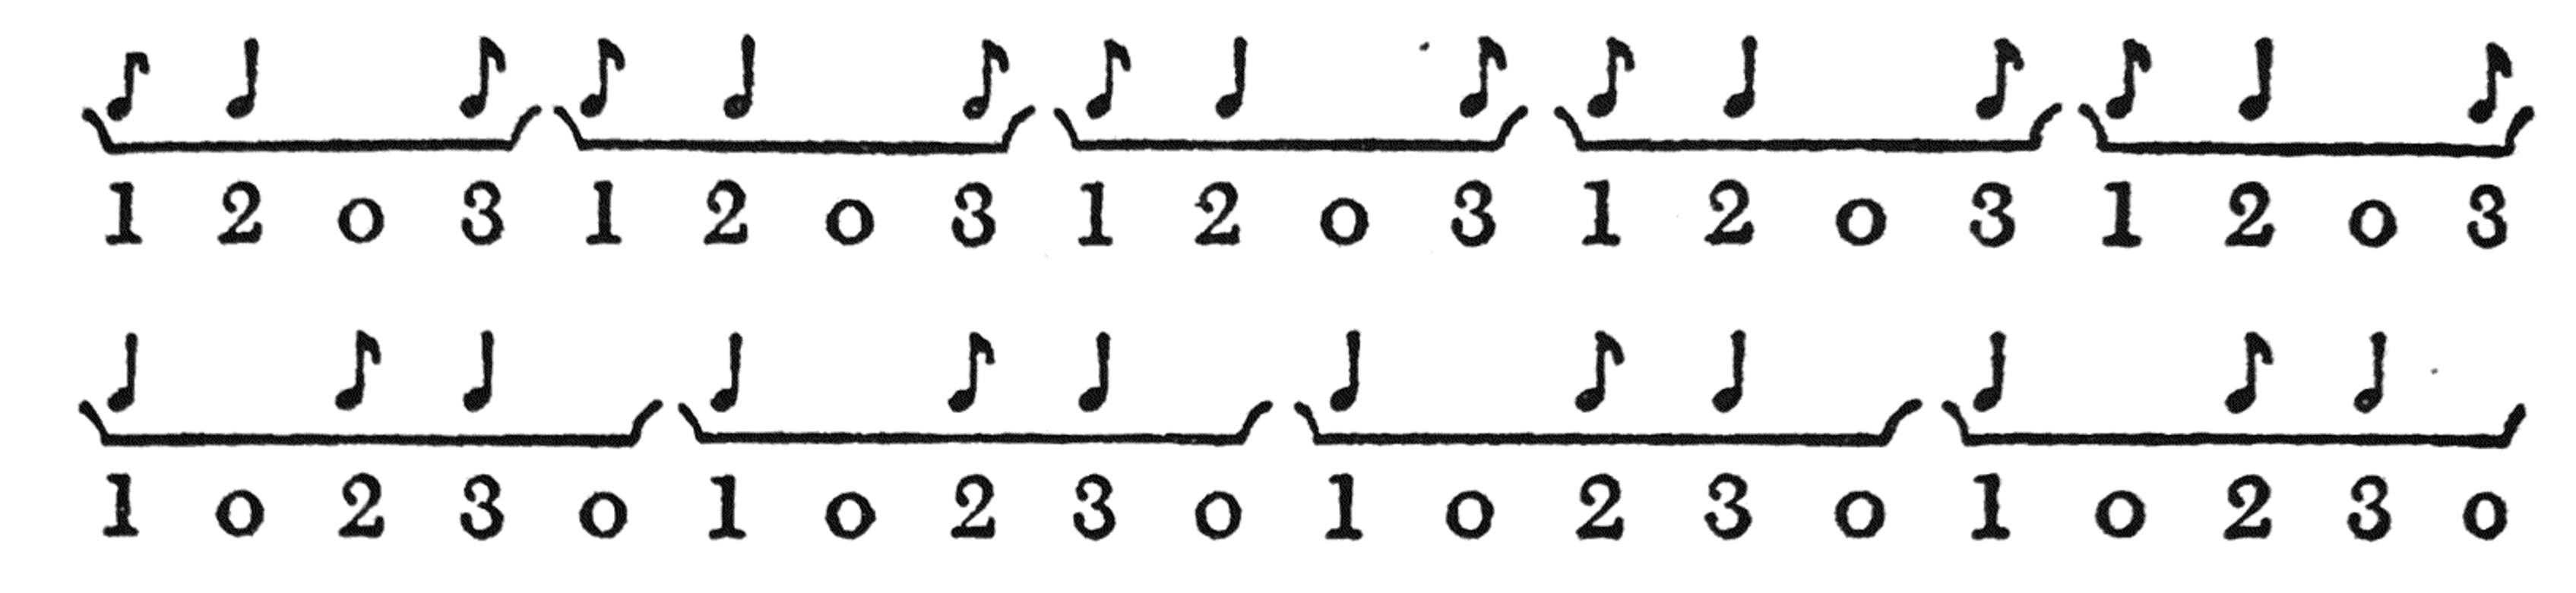
\includegraphics[
 width=0.7\textwidth]{./PDF/figure_19.pdf}
}
\caption{Curt Sachs (\textit{Rhythm and Tempo} p.108, 1979)\\
Example of overlap of two patterns. The same structure as African vertical hemiola can be observed.}
\label{fig:figure_19}
\end{figure}

According to our earlier definition of polyrhythm, this form is a cross-rhythm of 5-beat and 4-beat in a 20-beat cycle, and we can confirm similar rhythms in Indian music as well.

% %改ページや図版を章に収めたい場合は以下のように改ページすると収まる。
% \afterpage{\clearpage}
% \newpage

\subsubsection{Middle East}

According to \textit{Arab Music} by Salah al-Mahdi, Middle Eastern rhythms have rhythm patterns called iqa'. Mahdi describes Arab rhythms as "\textbf{a rhythm system peculiar to Arabic-speaking peoples}"\cite{mahdi:01} and "\textbf{originally linked to poetic meter (omitted), which gradually became somewhat independent}"\cite{mahdi:01}. Sachs also states that "\textbf{Arabian music originally followed the rhythm of poetry}"\cite{sachs:01}. Regarding the polyrhythmic nature of Middle Eastern music (Sachs refers to it as Near Eastern), Sachs states: "\textbf{When the three elements of sound—loudness, timbre, and beat—occur simultaneously, a complex aggregate of meter and accent is created within any single pattern that is almost polyrhythmic. It is infinitely variable in length, in the distribution of accent and timbre, and has varied}"\cite{sachs:01}. According to our earlier definition, while this is polyrhythmic in a broad sense, I was unable to find similar cases of the clear cross-rhythm forms seen in Indian music.

% 図\ref{fig:figure_20}にあるチェニジアの例を上げている。

% \begin{figure}[ht]
% \centerline{
% 	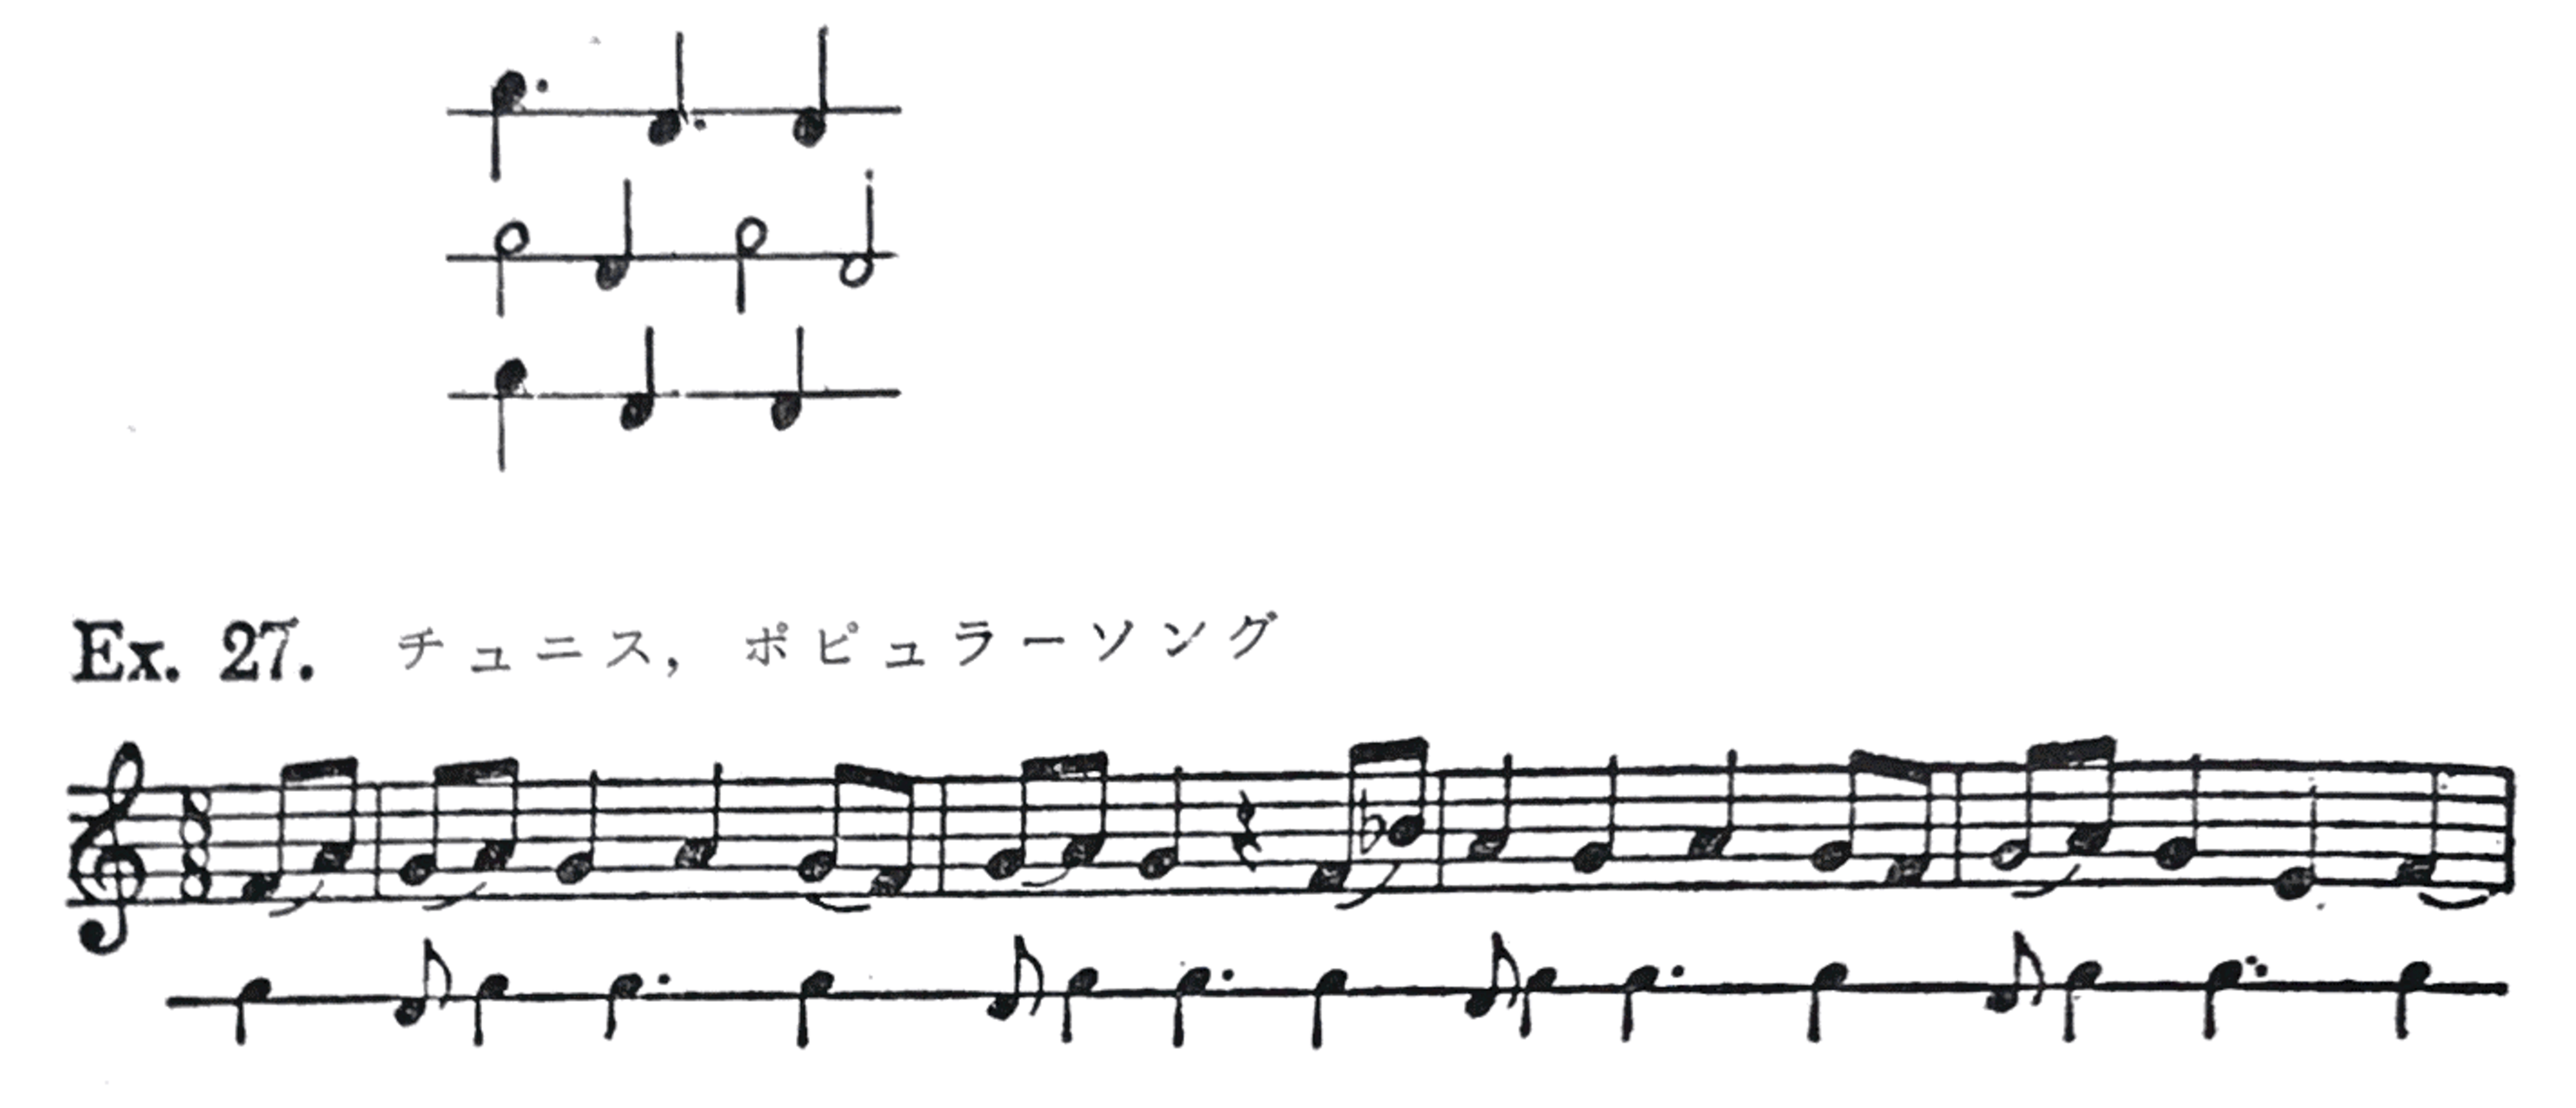
\includegraphics[
%  width=\textwidth]{./PDF/figure_20.pdf}
% }
% \caption{クルト・ザックス (『リズムとテンポ』p88, 1979)\\
% 譜例は上段の歌に対して下段のリズムが特に周り混むこともなくアフリカやインドの例のような明確なクロスリズムの形を持っていない}
% \label{fig:figure_20}
% \end{figure}

\subsubsection{Latin}

Regarding Latin rhythms, we will examine the clave, a rhythm pattern that is "\textbf{the cornerstone of Latin music}"\cite{yubi:01}, struck by claves, a percussion instrument from Central and South America. Tsukada states: "\textbf{What is interesting is that this standard rhythm pattern is thought to have formed the basis of the Latin music rhythms we often hear today}"\cite{tsukada:01}. He also points out the similarity: "\textbf{When examining the rhythms of Afro-Cuban music, for example rumba, in detail, there is a strong kinship between the clave and the standard rhythm pattern}"\cite{tsukada:01}. He also simultaneously points out that "\textbf{rumba preserves the characteristics of African rhythm structure extremely well, with 3-beat system (6/8 time or 12/8 time) rhythms and 2-beat system (2/4 time or 4/4 time) rhythms proceeding simultaneously in separate parts. In other words, it has a polyrhythmic structure}"\cite{tsukada:01}.

Figure \ref{fig:figure_21} shows this similarity and polyrhythmic structure. From this figure, it can be inferred that "\textbf{what occurs when trying to perform standard rhythm pattern A (author's note: referring to the standard rhythm pattern of 2-9 in the figure) not in the original 3-beat system but in a 2-beat system is the clave rhythm system}"\cite{tsukada:01}.

Furthermore, the rhythm called "tresillo" (Score 2-11 in Figure \ref{fig:figure_21}), derived from this clave, "\textbf{including its variations, has been extensively used not only in Latin music but also in rhythm and blues, jazz, rock and roll, and has had an enormous influence on the formation and development of popular music worldwide thereafter. And the rhythm that became the origin of this (omitted) was the standard rhythm pattern of traditional African music}"\cite{tsukada:01}. Thus, the African musical origins of popular music can be recognized "\textbf{not as subjective impressions or speculations with weak grounds, but as discourse consistent with historical facts derived from music analysis}"\cite{tsukada:01}. I believe this validates the methodology of approaching the development of popular music in this research from "polyrhythm/cross-rhythm" from a music historical perspective.

\begin{figure}[ht]
\centerline{
	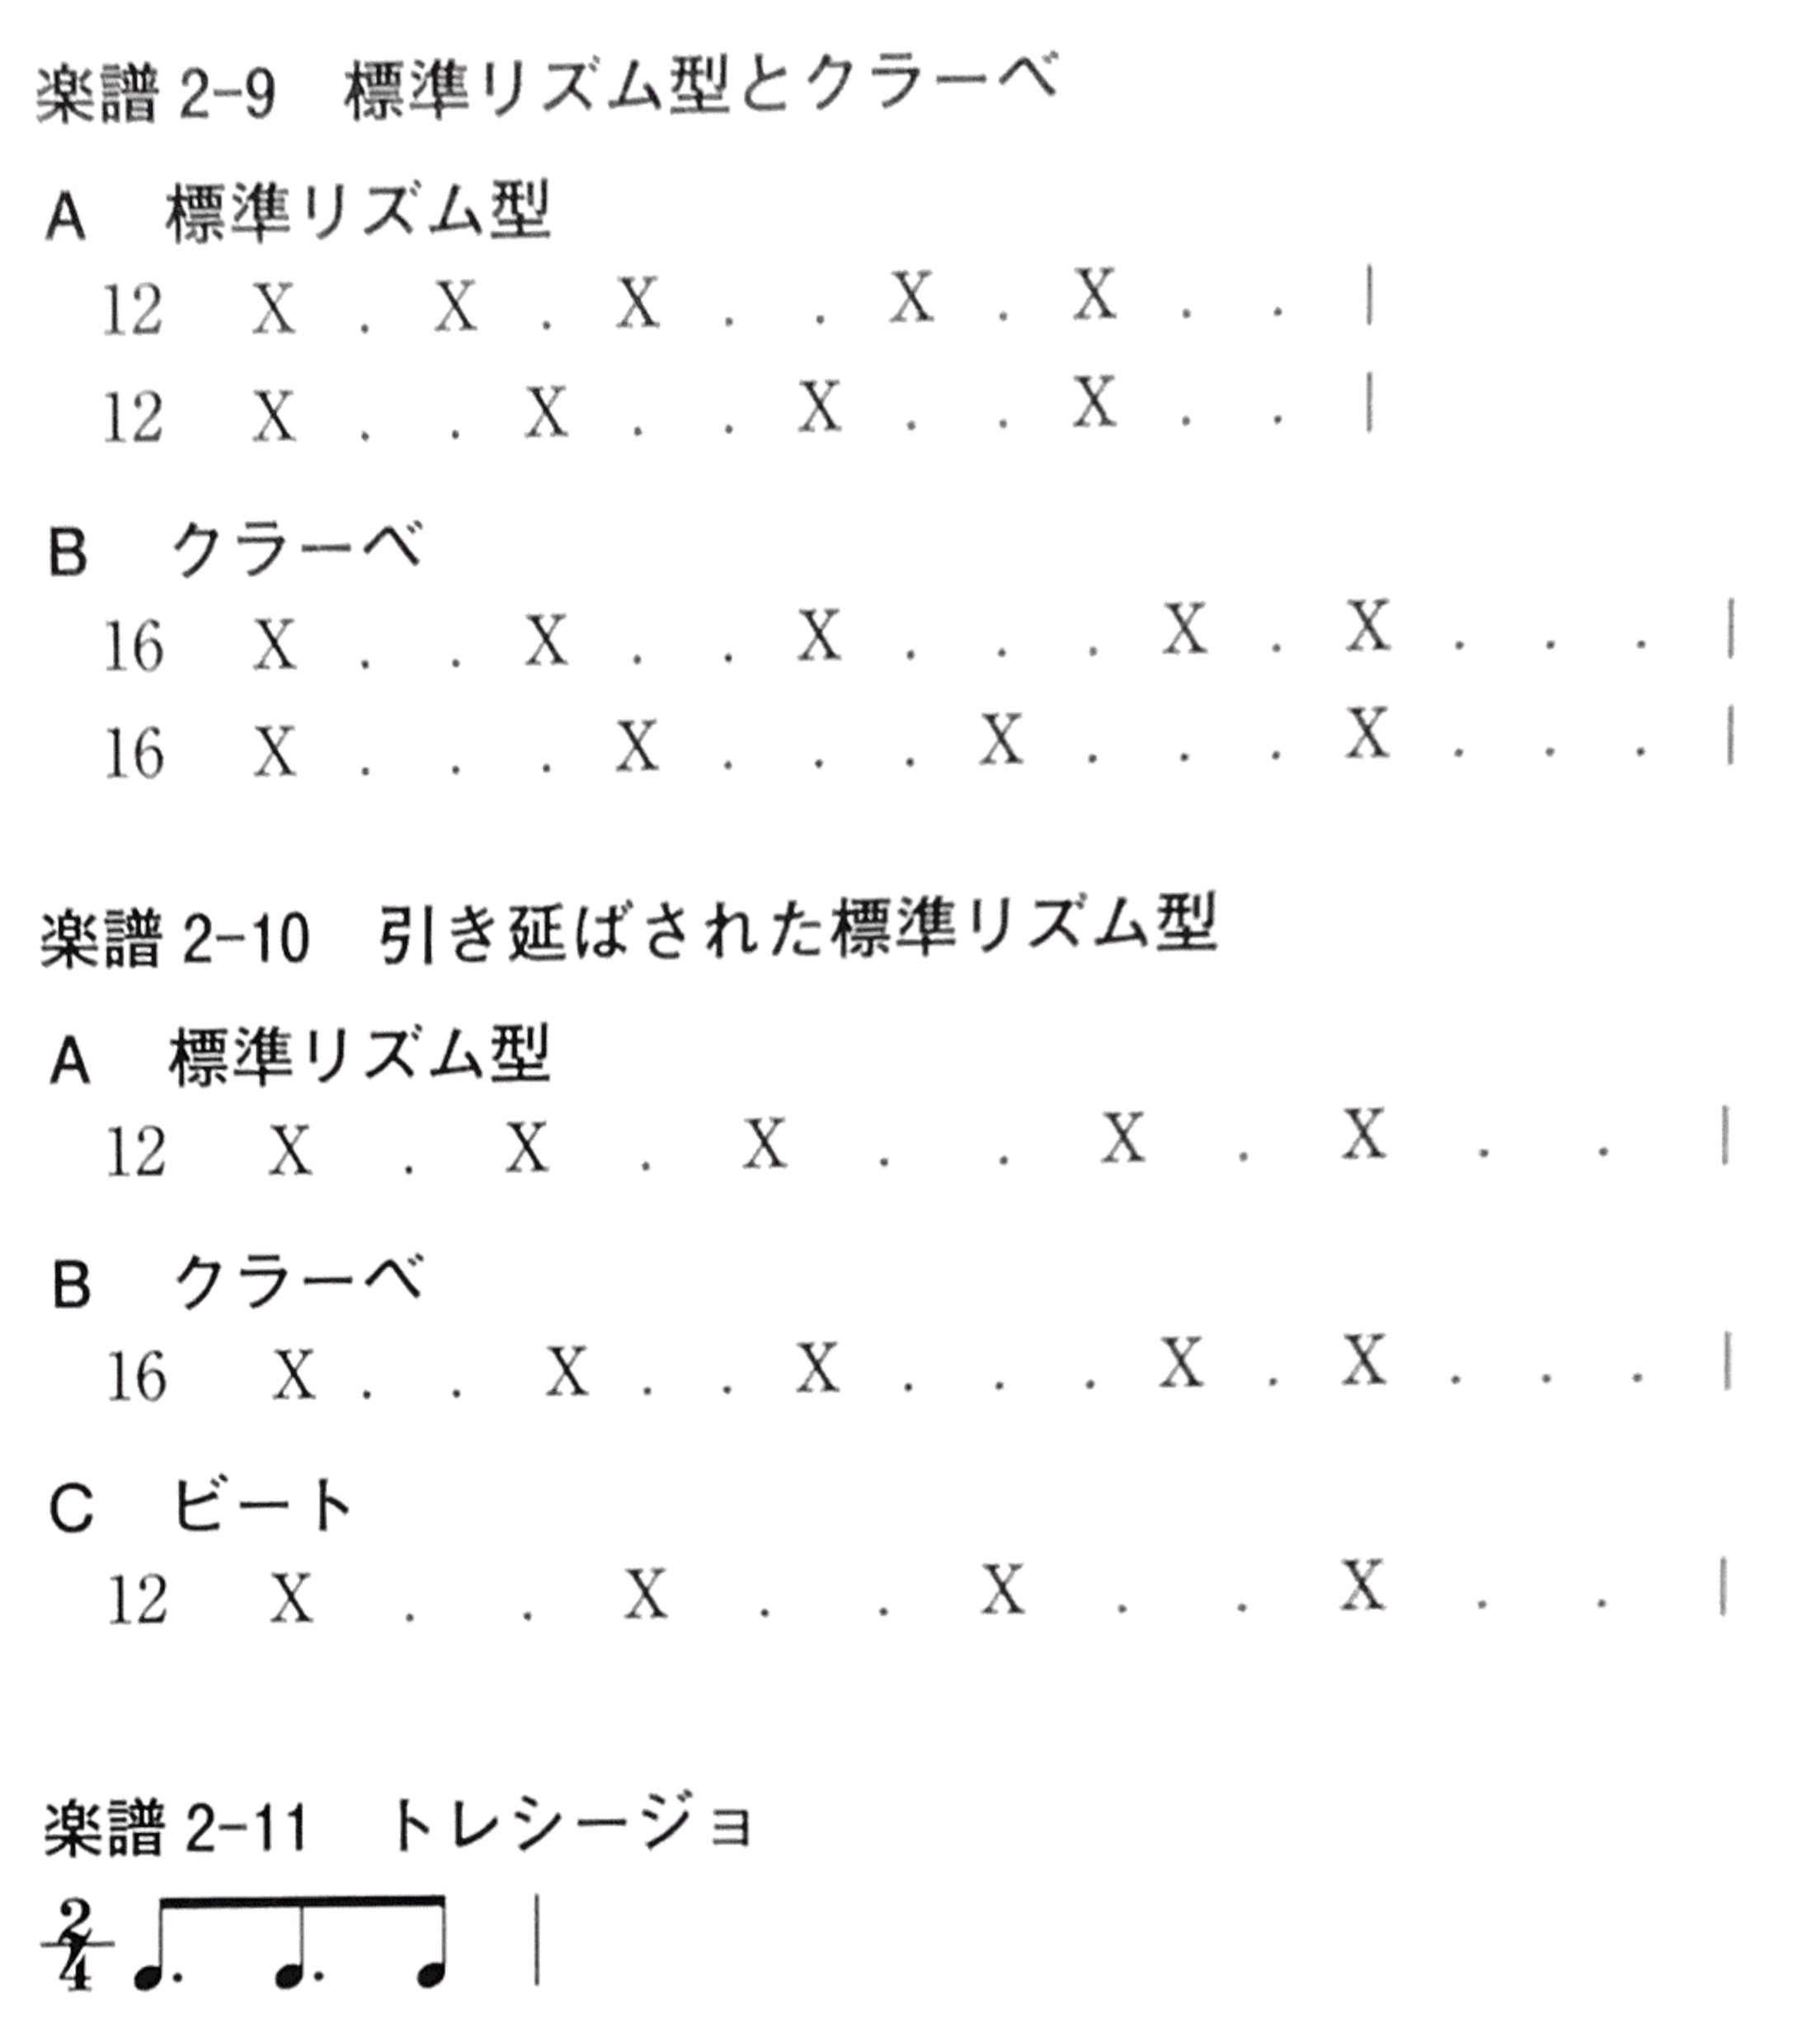
\includegraphics[
 width=0.75\textwidth]{./PDF/figure_21.pdf}
}
\caption{Kenichi Tsukada (\textit{The Truth About African Music} p.75 Scores 2-9, 2-10, 2-11, 2016)\\
Figures showing the similarity between African standard rhythm patterns and the clave, and tresillo patterns}
\label{fig:figure_21}
\end{figure}

Furthermore, the "polyrhythmic nature" of the clave and its relationship to "African basic rhythms" can be examined through rhythm strike points illustrated using waveforms in \textit{Rumba Clave: An Illustrated Analysis}. This analysis clearly shows the strike points of the clave in 4/4 time and 12/8 time, then compares the strike points of ten different performers. From this comparison, traces of Tsukada's "African origins of the clave" can be observed. Additionally, the fluctuation of strike points between 4/4 time and 12/8 time can be visually observed, and although it does not superficially take the form of cross-rhythm, the fact that the clave is of African origin and that such rhythm with "sway" and "accent" is one manifestation of the "African polyrhythmic stage" as cited in Kikuchi and Otani's definition of polyrhythm earlier. If "\textbf{Spanish-Cuban people who had not acquired the African-specific way of feeling the basic pulse of the standard rhythm pattern heard the standard rhythm pattern as a rhythm pattern consisting of 16 pulses}"\cite{tsukada:01}, then even according to our earlier definition, this can be said to be extremely polyrhythmic music.

\subsection{Polyrhythm/Cross-rhythm in Western Music}
\subsubsection{Western Music, Contemporary Music, American New Music \label{Western-Modern-AmericanNewMusic}}

Regarding "polyrhythm/cross-rhythm" in Western music, the \textit{New Music Dictionary} (40th edition, 1996) again states: "\textbf{Examples of polyrhythm (metric) are found mostly in the 14th-15th centuries and the 20th century, and this phenomenon is closely related to music being free from tonal function and functional harmony}"\cite{asaka:01}. Figure \ref{fig:figure_22} is the musical example illustrated there.

\begin{figure}[ht]
\centerline{
	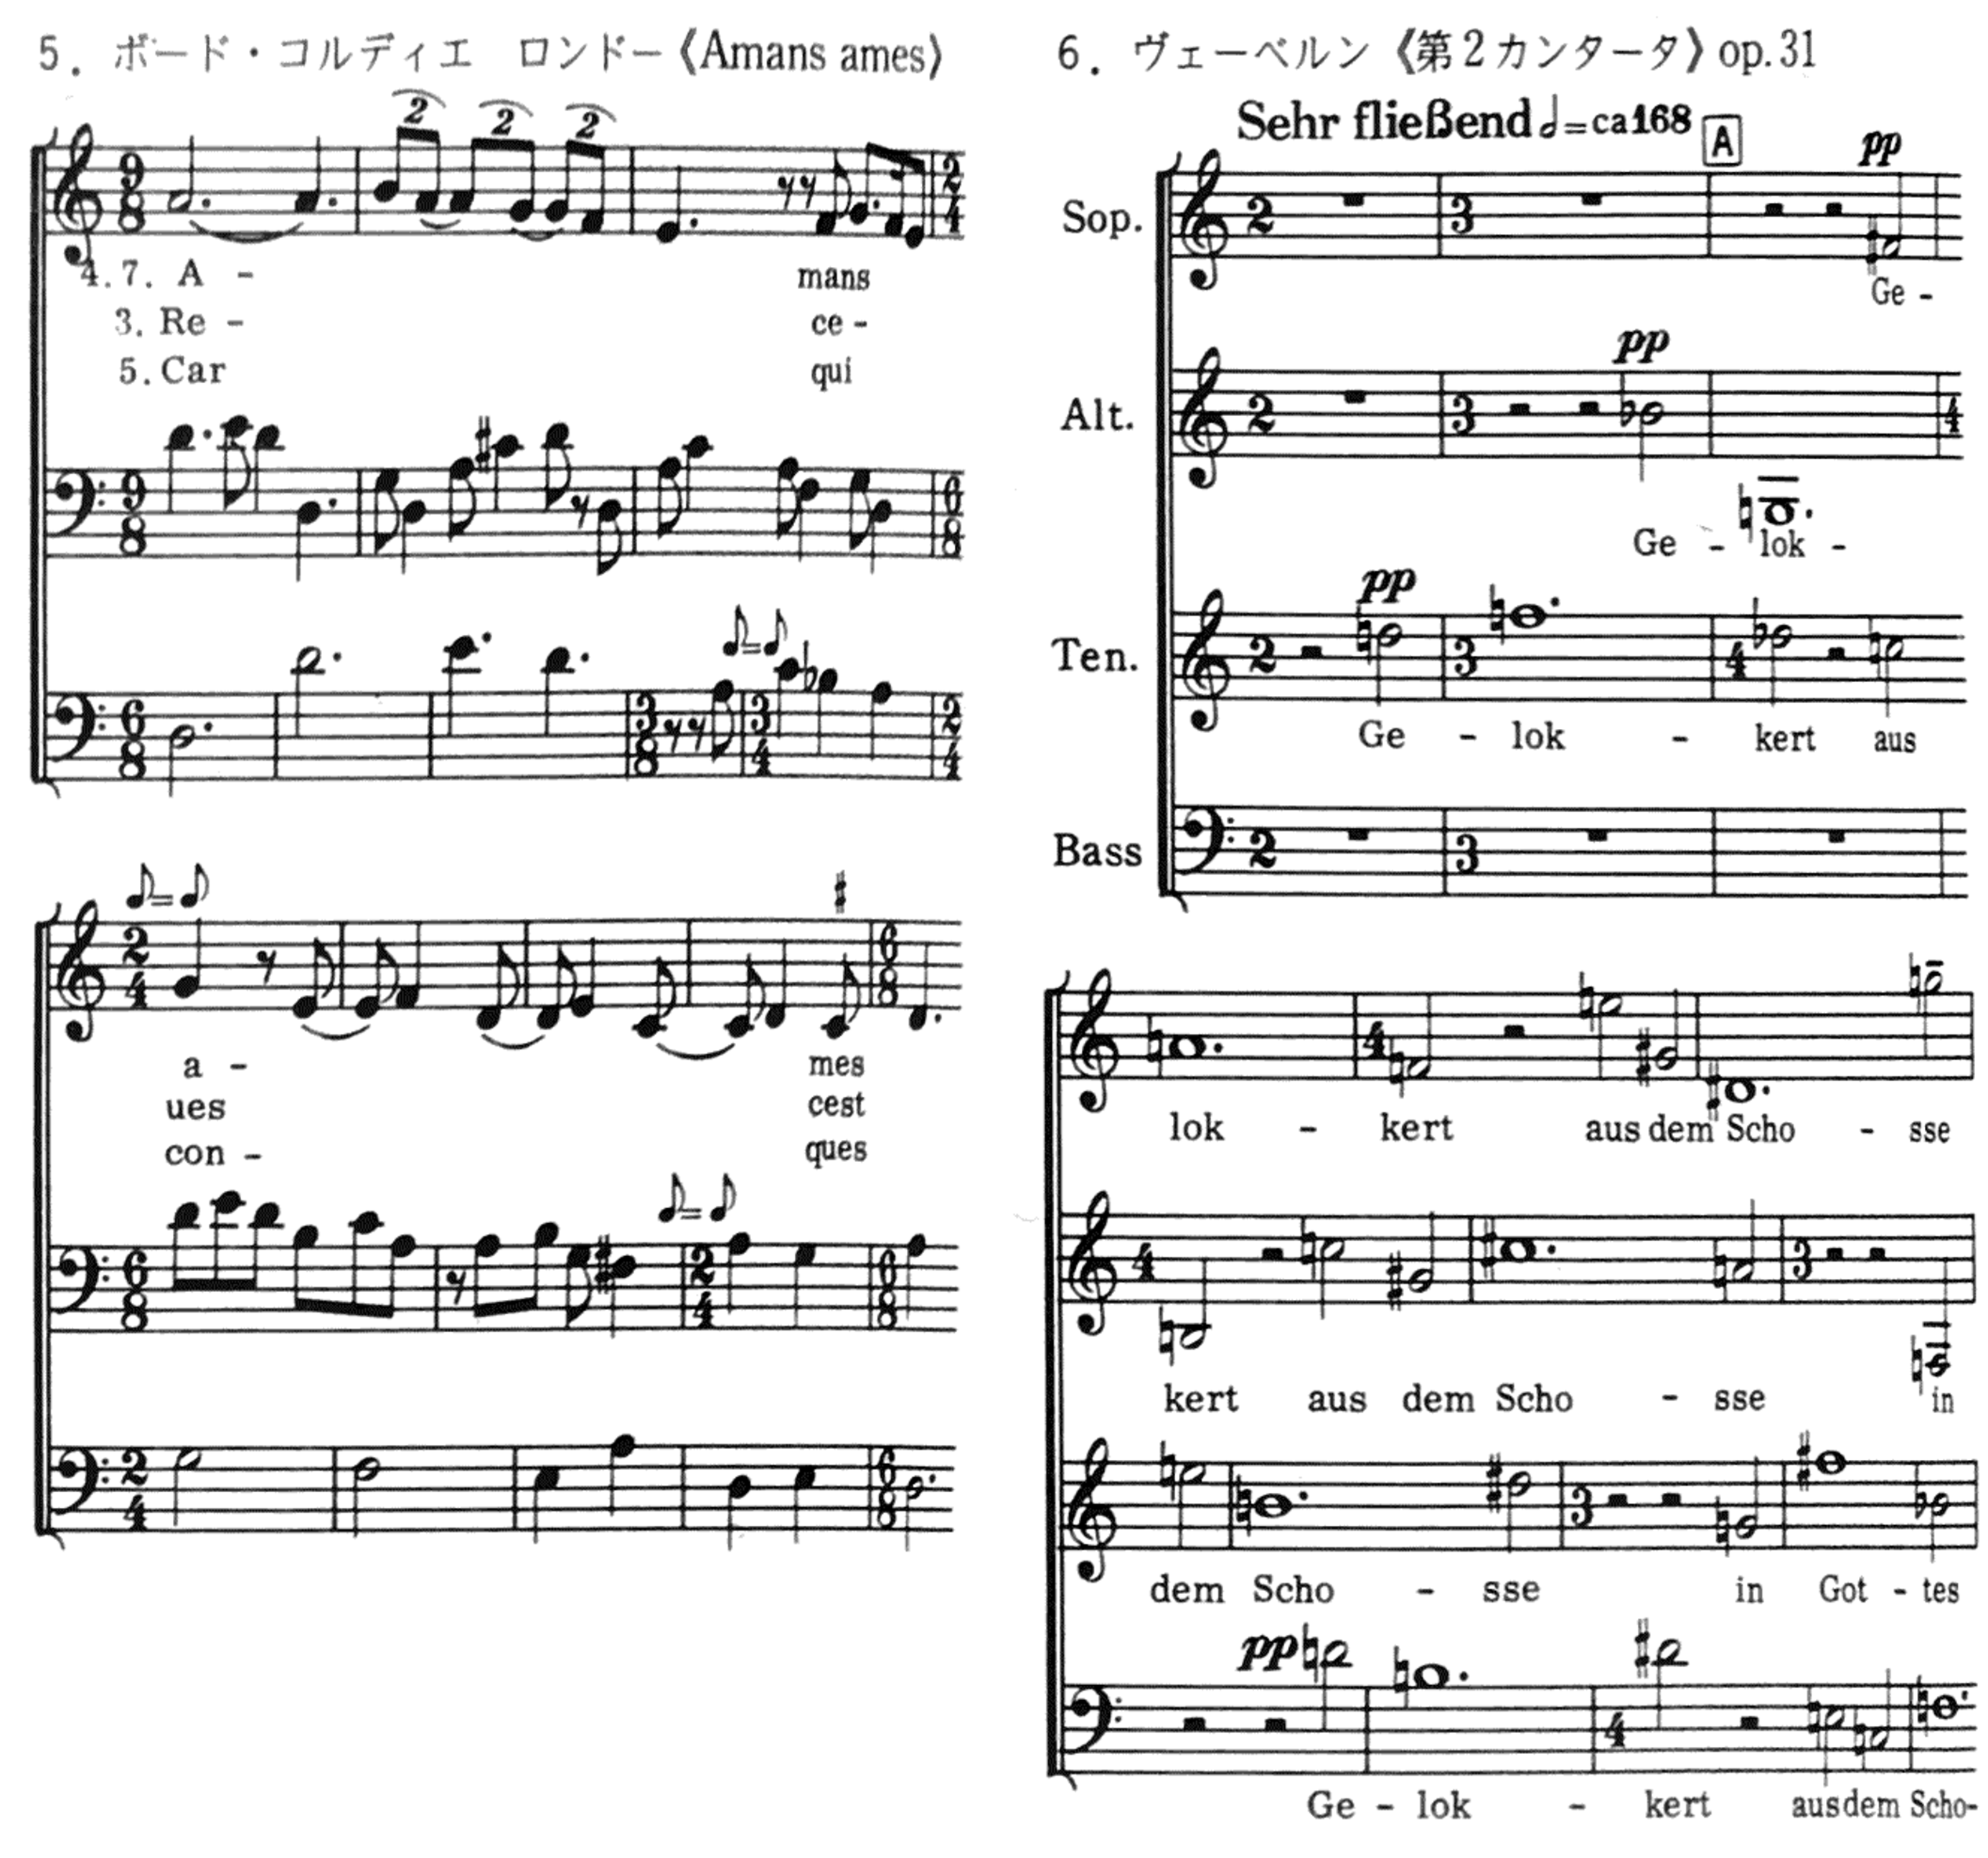
\includegraphics[
 width=0.75\textwidth]{./PDF/figure_22.pdf}
}
\caption{Jun Asaka (\textit{New Music Dictionary} p.538, Examples 5 and 6, 1977)\\
Example where bar lines wrap around due to different time signatures in different staves}
\label{fig:figure_22}
\end{figure}

Regarding the period before Baroque, Sachs's \textit{Rhythm and Tempo} also addresses polyrhythm up to the Renaissance with "alternation of meter" and "flamboyant polyrhythm," citing examples from late Renaissance composer Cipriano de Rore's "Vergine pura" (Figure \ref{fig:figure_23}).

\begin{figure}[ht]
\centerline{
	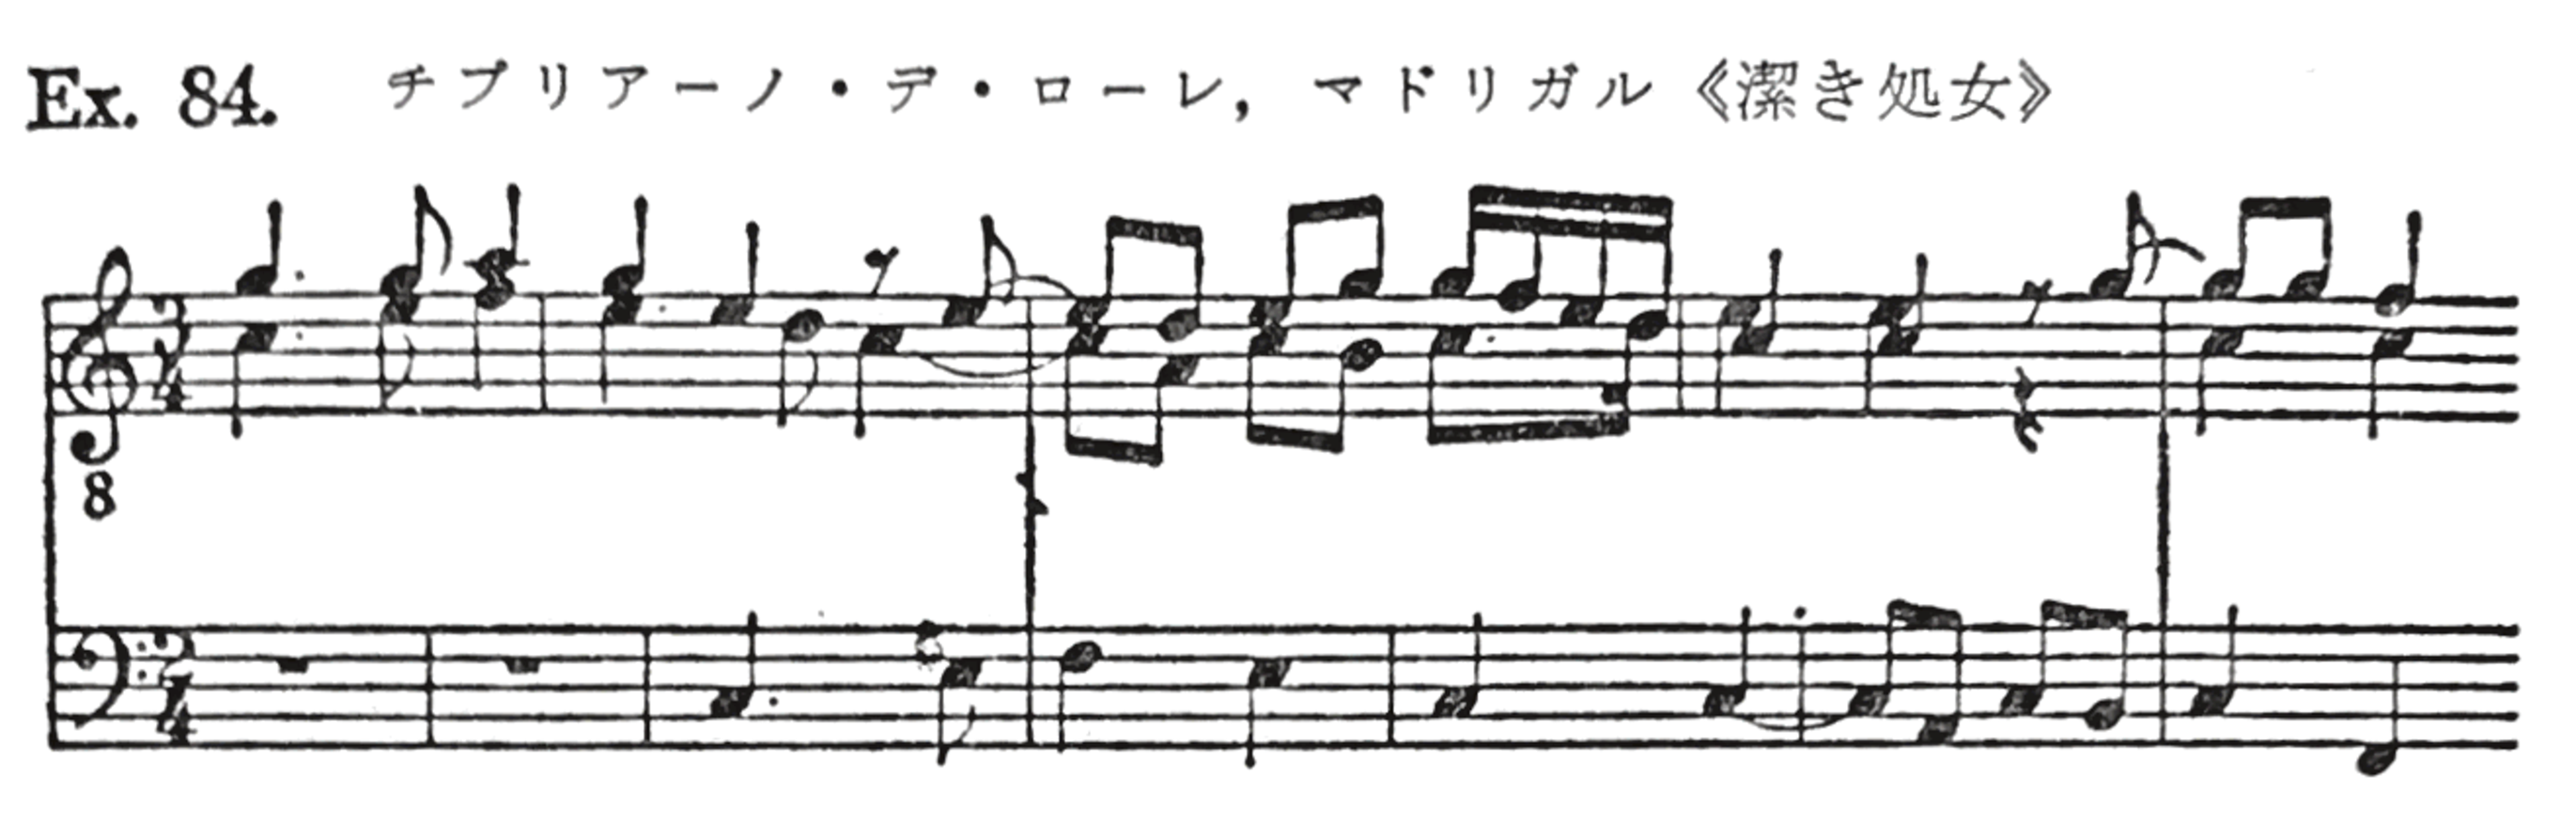
\includegraphics[
 width=0.75\textwidth]{./PDF/figure_23.pdf}
}
\caption{Curt Sachs (\textit{Rhythm and Tempo} p.272 Ex. 84, Cipriano de Rore's "Vergine pura" example, 1979)\\
Like Figure \ref{fig:figure_22}, bar lines wrap around due to different time signatures in different staves, but no form like cyclical rhythm patterns is observed}
\label{fig:figure_23}
\end{figure}

Entering the Baroque period, "polyrhythmic/cross-rhythmic" rhythms can be observed in hemiola structures in relation to dance, but cannot be seen as characteristic of musical rhythm. Furthermore, although 4/4 time established its leading position during the Baroque period, this also became the foundation for rhythms in subsequent Western music and popular music. Reich points out: "\textbf{What can be said about Baroque music in general, but especially Bach, is that the beat is constant and basically there is no ritardando or accelerando (omitted). What should be done is to maintain tempo}"\cite{strickland:01}, from which it can be understood that Baroque period rhythms had ceased to possess polyrhythmic elements.

Entering the 20th century, Reich can be recalled as one of the contemporary music composers who approached "polyrhythmic/cross-rhythmic" rhythms. While phase shifting is Reich's representative technique taken up here, Reich speaks in interviews about how phase shifting is a variation of canon form, inspired by tape loop works ("\textbf{Oh my God! This relationship is amazing. But what is really interesting is the process of starting in unison and slowly going out of phase, which is actually a variation of the old Western music canon!}"\cite{obrist:01}). In the same interview, Reich states: "\textbf{When I performed with Arthur Murphy, who became a founding member of my first ensemble, we discovered that we could play without using tape. This was in 1967, and this became a major breakthrough, leading to 'Piano Phase,' 'Violin Phase' (1967), and subsequently 'Drumming' (1970-1971)}"\cite{obrist:01}, describing his series of phase shift works as canons characterized by temporal change that "shifts" rather than the "sway" or "accent" of African polyrhythm. However, when asked in another interview about the relationship with his experience learning Gamelan music, Reich states: "\textbf{(author's note: regarding Music for Mallet Instruments, Voices and Organ) I certainly listened to various recordings. Another example is 'Drumming.' I didn't write it because I went to Ghana. (omitted) The African element in that work—the repetitive pattern in 12/8 time—was already done in 'Piano Phase' and 'Violin Phase' in 1967. I went to Africa to confirm}"\cite{strickland:01}, using the basic African rhythm structure of 12/8 time repetition while denying that this was influenced by African music itself, stating it was influenced by earlier works. Therefore, I consider it difficult to position Reich's works within the earlier definition of "polyrhythm/cross-rhythm" from the composer's own views (interviews).

\subsection{Polyrhythm/Cross-rhythm in Popular Music}

Thus far, we have examined, albeit in a limited manner, rhythms practiced in Africa, India, the Middle East, Latin America, and Western music. To comprehensively discuss music, it could be said to be impossible unless one examines all examples of that music. Furthermore, regarding popular music, since it is music that is currently in progress, even if we limit its origins to American folk music such as jazz and blues, the difficulty of discussing it comprehensively increases dramatically. Therefore, we will introduce the activities of Kikuchi, one of the authors whose writings form the basis for this thesis's polyrhythm definition, between Kikuchi and Otani.

When examining Naruyoshi Kikuchi's activities, it becomes clear that he has performed numerous practical works and performances through polyrhythmic approaches. Here, we will take up \textit{Date Course Pentagon Royal Garden} (now dCprG) as one example. In \textit{The School That Taught Sensuality and Melancholy}, Kikuchi states about his musical piece \textit{PLAYMATE AT HANOI}\cite{works-kikuchi:01}: "\textbf{It's a cross of 4 and 3. (omitted) Integer polyrhythm}"\cite{kikuchi-ootani:01}. He does say that as the piece progresses, "4 and 3 become mixed," but this part of his statement indicates that this piece is first in a state of vertical hemiola, and according to this thesis's definition, in a state of "cross-rhythm."

Then, regarding the rhythm structure of \textit{structure I la structure de la magie monderne / Structure 1 (Structure of Modern Magic)}\cite{works-kikuchi:02} by the same band, he explains as follows in comparison to the earlier \textit{PLAYMATE AT HANOI}: "\textbf{The structure here is 4/4 and 5/4. That is, the feature is that 4-beat and 5-beat coexist, (omitted) not the divisible cosmos polyrhythm of 12 prime numbers like the previous work 'Playmate at Hanoi,' but a rhythm that sounds square from one perspective (taking it in 5-beat, it sounds like house music based on sixteenth notes), but sounds 'accented' from the other perspective (taking it in 4-beat, a stumbling tribal rhythm like Tsugaru folk song or African folk song can be heard). The brass riff is also made entirely of variations of only sixteenth notes, but because strike points are frequently placed at unusual strike points, there is an intention to mix the instability and pleasure of the step. Furthermore, the long melody of the synthesizer that appears first as magic is composed of triplets, and in terms of integer approximation, triplets are positioned between 4-beat and 5-beat, working like an adhesive between the two rhythms.}"\cite{kikuchi:01}. This explanation corresponds to an example that matches this paper's definition of "polyrhythm" based on Kikuchi and Otani's definition.

Even without such clear examples, the connection from African basic rhythms to Latin clave discussed earlier in the section on Latin music, and the fact that this has widely influenced popular music, also demonstrates that popular music constantly receives African polyrhythmic sensibility. Furthermore, looking at jazz, which was popular music of the early 20th century, comparing Western music and jazz, "\textbf{whereas in classical music all parts are dominated by harmony and interlock vertically with each other, in jazz, while dominated by harmony, the rhythm of each part is linearly or horizontally independent, often forming polyrhythm}"\cite{yubi:01}, which also suggests the influence of African polyrhythmic sensibility. Yubi also points out that "\textbf{the bebop movement beginning in the 1940s aimed to expand the degree of expression in improvisation, and by introducing accent shifts of small note values, formed a more powerful polyrhythm than swing feel}"\cite{yubi:01}. As an example of post-bebop jazz musicians' African polyrhythmic sense, Figure \ref{fig:figure_24} shows part of John Coltrane's solo in \textit{Bye Bye Blackbird}\cite{miles:03}. Here, Coltrane uses phrases in triplets over two beats on a 4/4 rhythm, expressing 6-beat time over 4-beat time.

\begin{figure}[ht]
\centerline{
	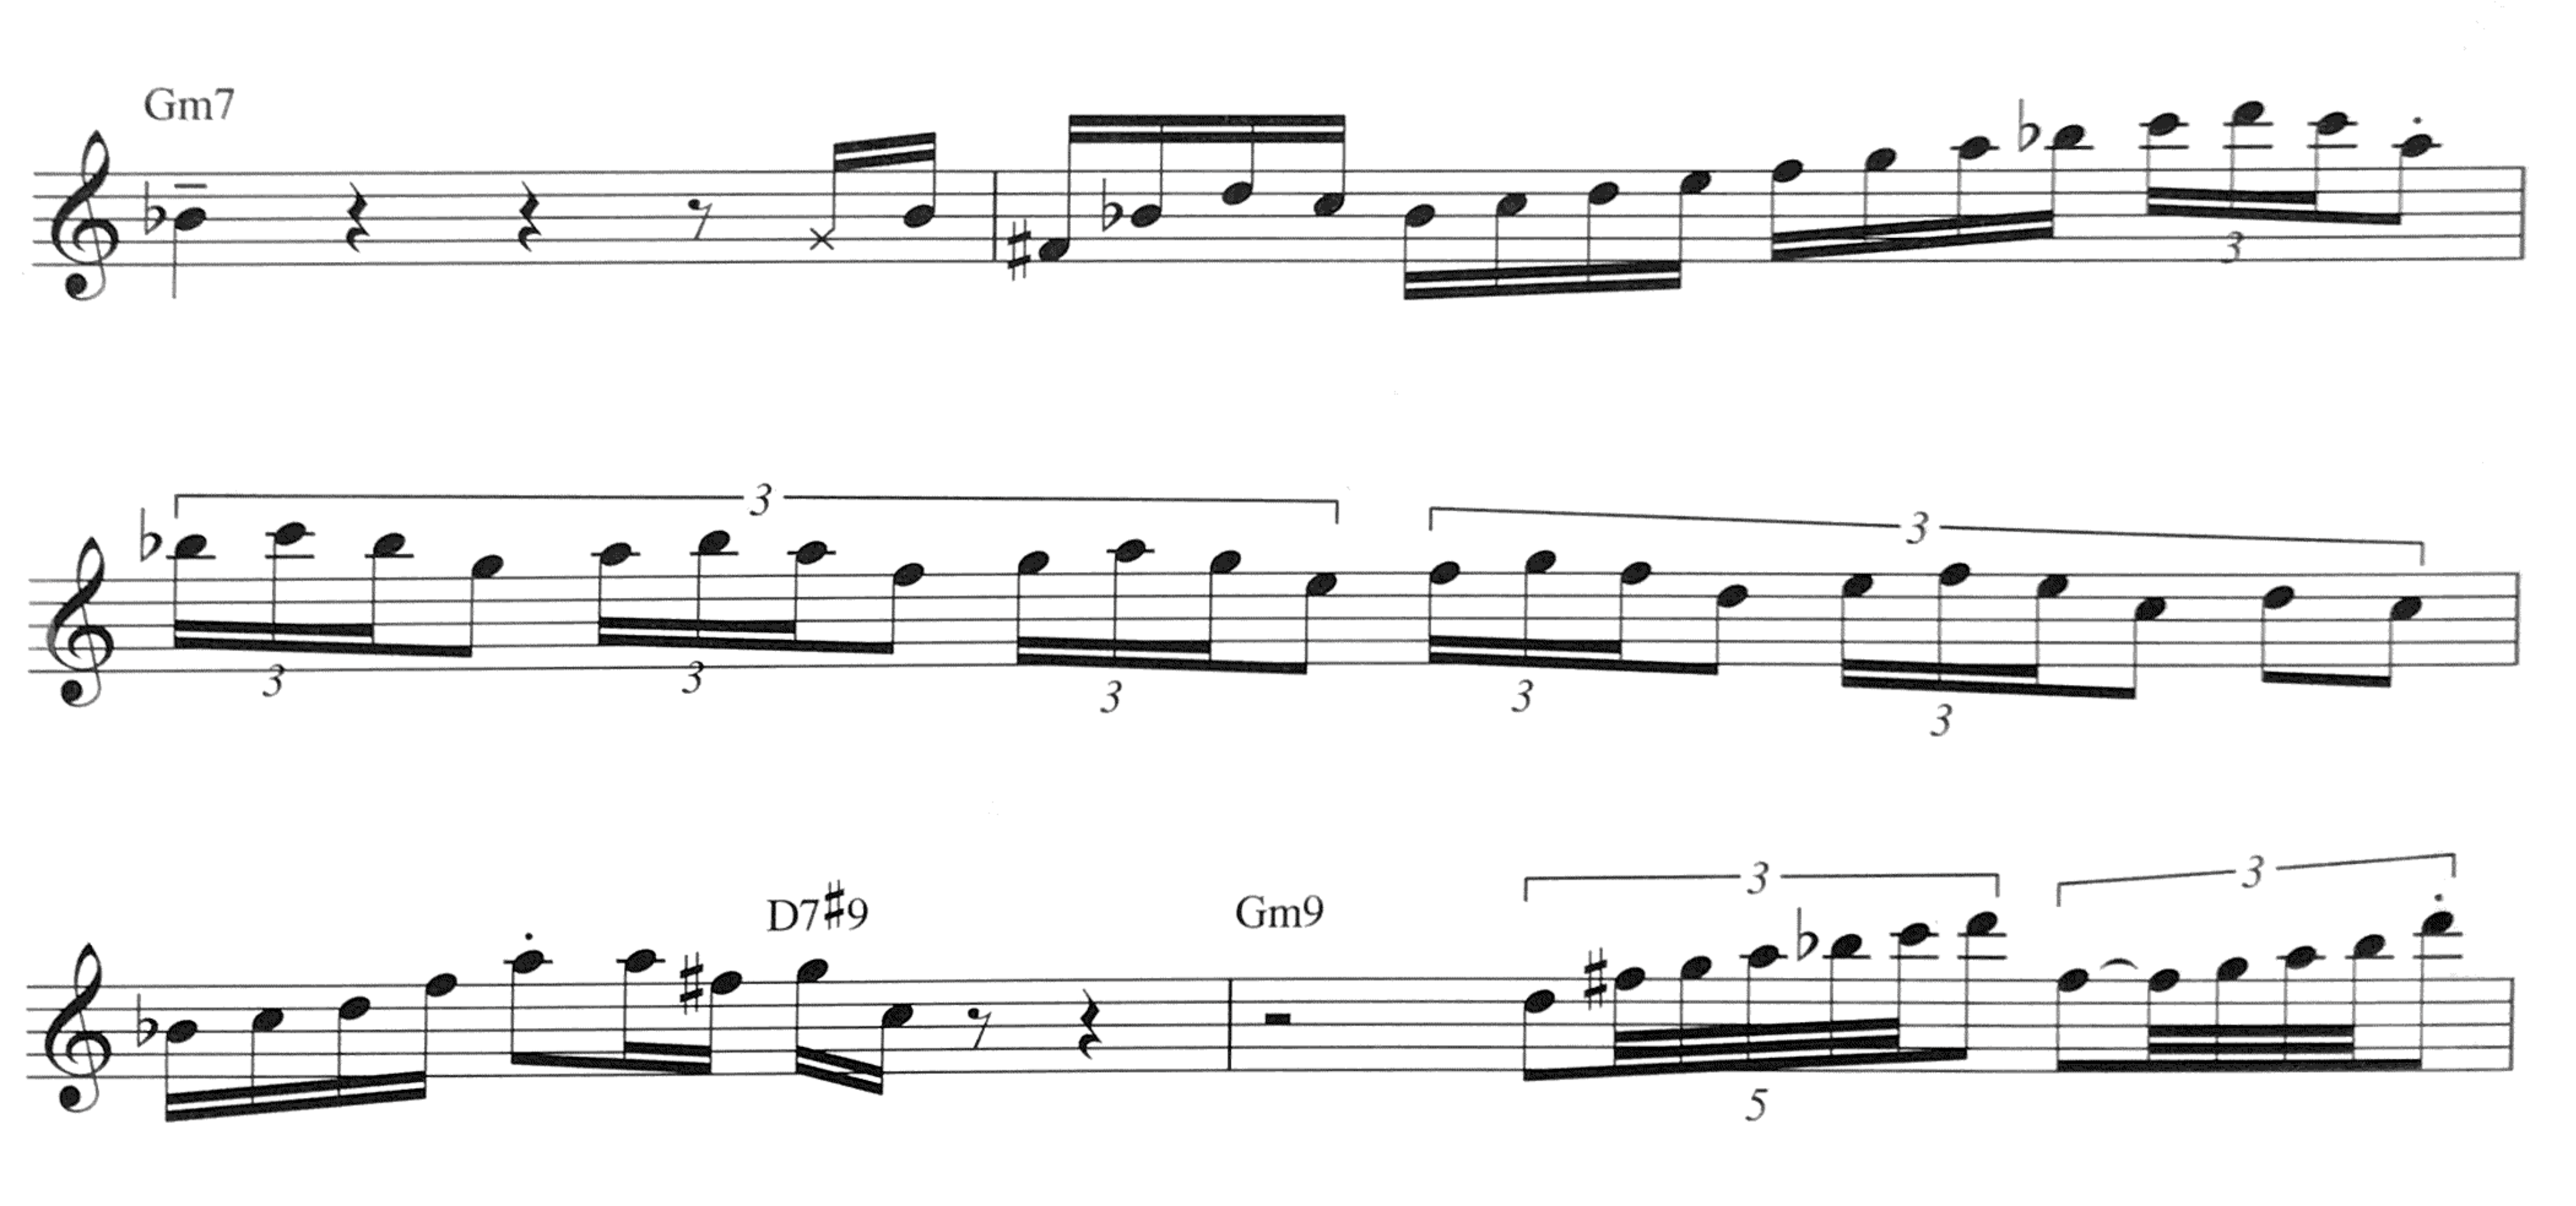
\includegraphics[
 width=\textwidth]{./PDF/figure_24.pdf}
}
\caption{Hal Leonard Corp (\textit{John Coltrane Omnibook: For C Instruments} p.50, excerpt from solo transcription of \textit{Bye Bye Blackbird}, 2013)\\
In the second measure of Example 3, entering with a 4-beat phrase in sixteenth notes, and using the phrase shape from the fourth beat of the same second measure as a motif, it becomes triplets over two beats in the third measure, dividing 4 beats into 6}
\label{fig:figure_24}
\end{figure}

Examples like Kikuchi's, where such division is applied throughout the entire piece, are not commonly found. However, entering the 21st century, the rhythmic "sway" and "accent" pointed out by Kikuchi and Otani have become increasingly observed, beginning with Robert Glasper's \textit{Black Radio}\cite{Glasper:02} released in 2012, and this can be said to be evidence of Kikuchi and Otani's definition as a contemporary manifestation of the African rhythmic sense that underlies popular music.

% ビジェイアイアー
%
% クラクラ
%
% これら総じて「揺れ」「訛り」をもった「ポリリズム的なリズム感覚」といっていいだろう。

% \subsection{考察}
%
% ーーーー執筆内容ーーーー\\
% 「ポリリズムやクロスリズムに関して人類はすでにこのようなことをやってきた。そして、それは事実、身体化可能なものだった」ということを説明したい\\
% クラシックの小節線ずれこみなども、基本的に周りこむ場合には拍が共有される場合が多く、アフリカンポリなどの訛りがあるポリの常態では小節線が共有される場合が共通して見られることを指摘する。そこに現代的なグルーブ感やリズム認知があると考えることが出来る。そこにはクラーゲスが言う「拍子(タクト)が同一のものを反復するとすれば、リズムでは類似が回帰する」ということに対するリズム回帰する力がポピュラー音楽に於いて強く働いていると仮説をたてる。\\
% ーーーー執筆内容ーーーー\\
%
% ここまでポリリズム/クロスリズムというリズムについてのアプローチを見てきた。
%
% またこの事は、五線譜による記譜法が17世紀以降に確立され、同時期に平均律による調性と和声に重きが置かれるようになったバロック時期には見られなくなったことを

% \section{現代の音楽制作環境と考察}
%
% 次に、先のポリリズム/クロスリズムの状況を現代の音楽制作環境から考察していく。考察にあたってはポピュラー音楽に於ける楽理、楽譜、制作環境としてのソフトウェアを取り上げる。
%
% \subsection{楽理的考察}
%
% ーーーー執筆内容ーーーー\\
% ハーモニックリズム、ドミナント進行、コードの共有、が一定のリズムフィギュア、もしくは小節という単位、にのってる点をバークリー理論や作曲法を引き合いに出して述べる。このあたりはザックスの本から拾えないか??\\
% ーーーー執筆内容ーーーー\\
%
% バロックでのリズムと和声の密接と4分の4拍子の支配的
%
% バークリー理論でのポピュラー音楽への展開
%
%
%
% \subsection{楽譜的考察}
%
% ーーーー執筆内容ーーーー\\
% で、上記の話を記述する楽譜自体が「拍と小節線の共有」という、所謂「行進」のような話とそういう音楽を記述する上で発展してきた背景が、システムとして全体を縛っている、という話を進める。ここは先の4/4が支配的になった話をして譜面のシステムとしての完成と自由度のバーターを論じる。\\
% ーーーー執筆内容ーーーー\\
%
% \subsection{ソフトウェア的考察}
%
% ーーーー執筆内容ーーーー\\
% その楽譜の考えかたで現代のソフトウェアは出来ているので、多様性が生じ難い土壌になっている。その上でそういう音楽がマスで流通するのだから、より4/4の支配力が増してるだろう事を指摘する。\\
% ーーーー執筆内容ーーーー\\

%改ページや図版を章に収めたい場合は以下のように改ページすると収まる。
\afterpage{\clearpage}
\newpage

\section{Music with Multilayered Temporal Structures}

Based on the research on polyrhythm/cross-rhythm presented above, the following points were taken into consideration when composing the work.

\begin{enumerate}
  \item The definition of polyrhythm: "having beats that are not divisible by integers"
  \item Making this possible through simple rules
  \item Being able to control the sense of groove
\end{enumerate}

These considerations are based on the work titled ''{\bf New York 2997}''\cite{yamato:05}, which the author presented in 2016, where multiple rhythmic cycles wrap around periodically. As can be seen from the explanations so far, polyrhythm/cross-rhythm often exhibits a state where "rhythm fluctuates within a given measure," but I attempted to perform this movement, which is confined within measures, across bar lines. As the author stated in the introduction, if 4/4 meter is dominant in many musical pieces, I thought that by changing the way this 4/4 meter is used, it would be possible to present a sense of rhythm different from existing polyrhythms.

As a prototype for this purpose, I first developed a plugin called ''dc.PolyDelay20'' that runs on Ableton Live. Figure~\ref{fig:figure_25} shows a screenshot of its interface.

\begin{figure}[ht]
\centerline{
	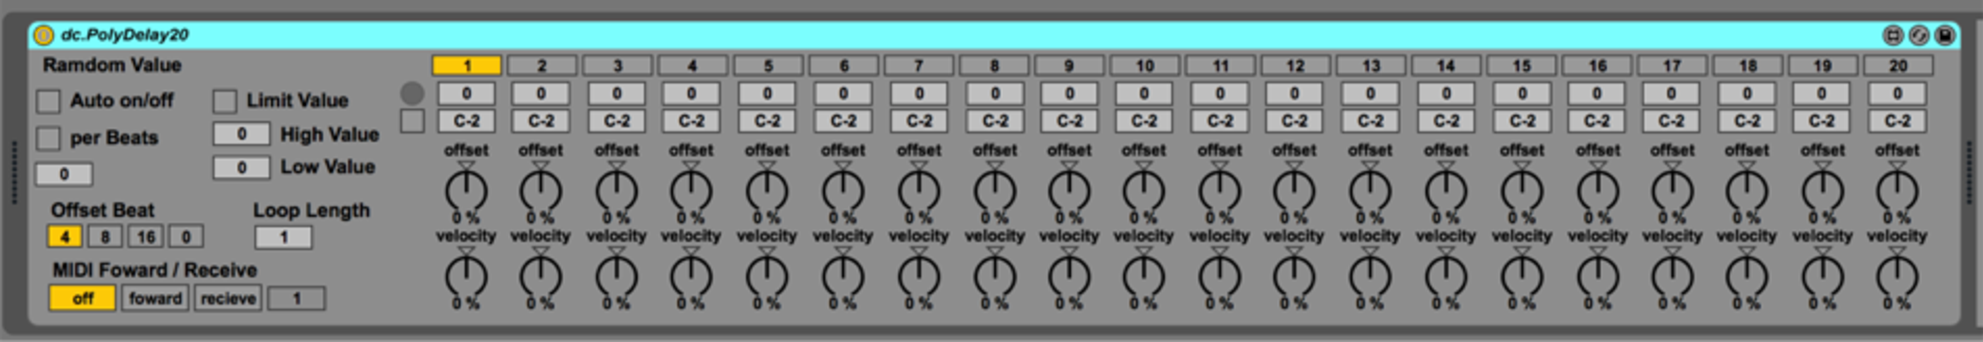
\includegraphics[
 width=\textwidth]{./PDF/figure_25.pdf}
}
\caption{Interface of dc.PolyDelay20}
\label{fig:figure_25}
\end{figure}

This plugin uses MIDI information input as a trigger. By using delay to specify and play up to 20 locations within a specific beat length, it can divide the beat and produce sound at specific timings. Additionally, since pitch information can be varied at that time, it is possible to generate phrases. I repeated prototypes using this plugin. At this time, I created ''{\bf Piano Etude}''\cite{yamato:06} and ''{\bf Percussion Ensemble}''\cite{yamato:07} as compositional prototypes for dividing a certain number of beats into 4 beats. These pieces are created by layering phrases in which lengths from 4 to 13 beats are each divided into 4 beats. The phrases for each piece are shown in Figure~\ref{fig:figure_26} (the same can be downloaded from this URL: \url{https://goo.gl/g3EvW1}) and Figure~\ref{fig:figure_27} (the same can be downloaded from this URL: \url{https://goo.gl/J23Pwi}).

\begin{figure}[ht]
\centerline{
	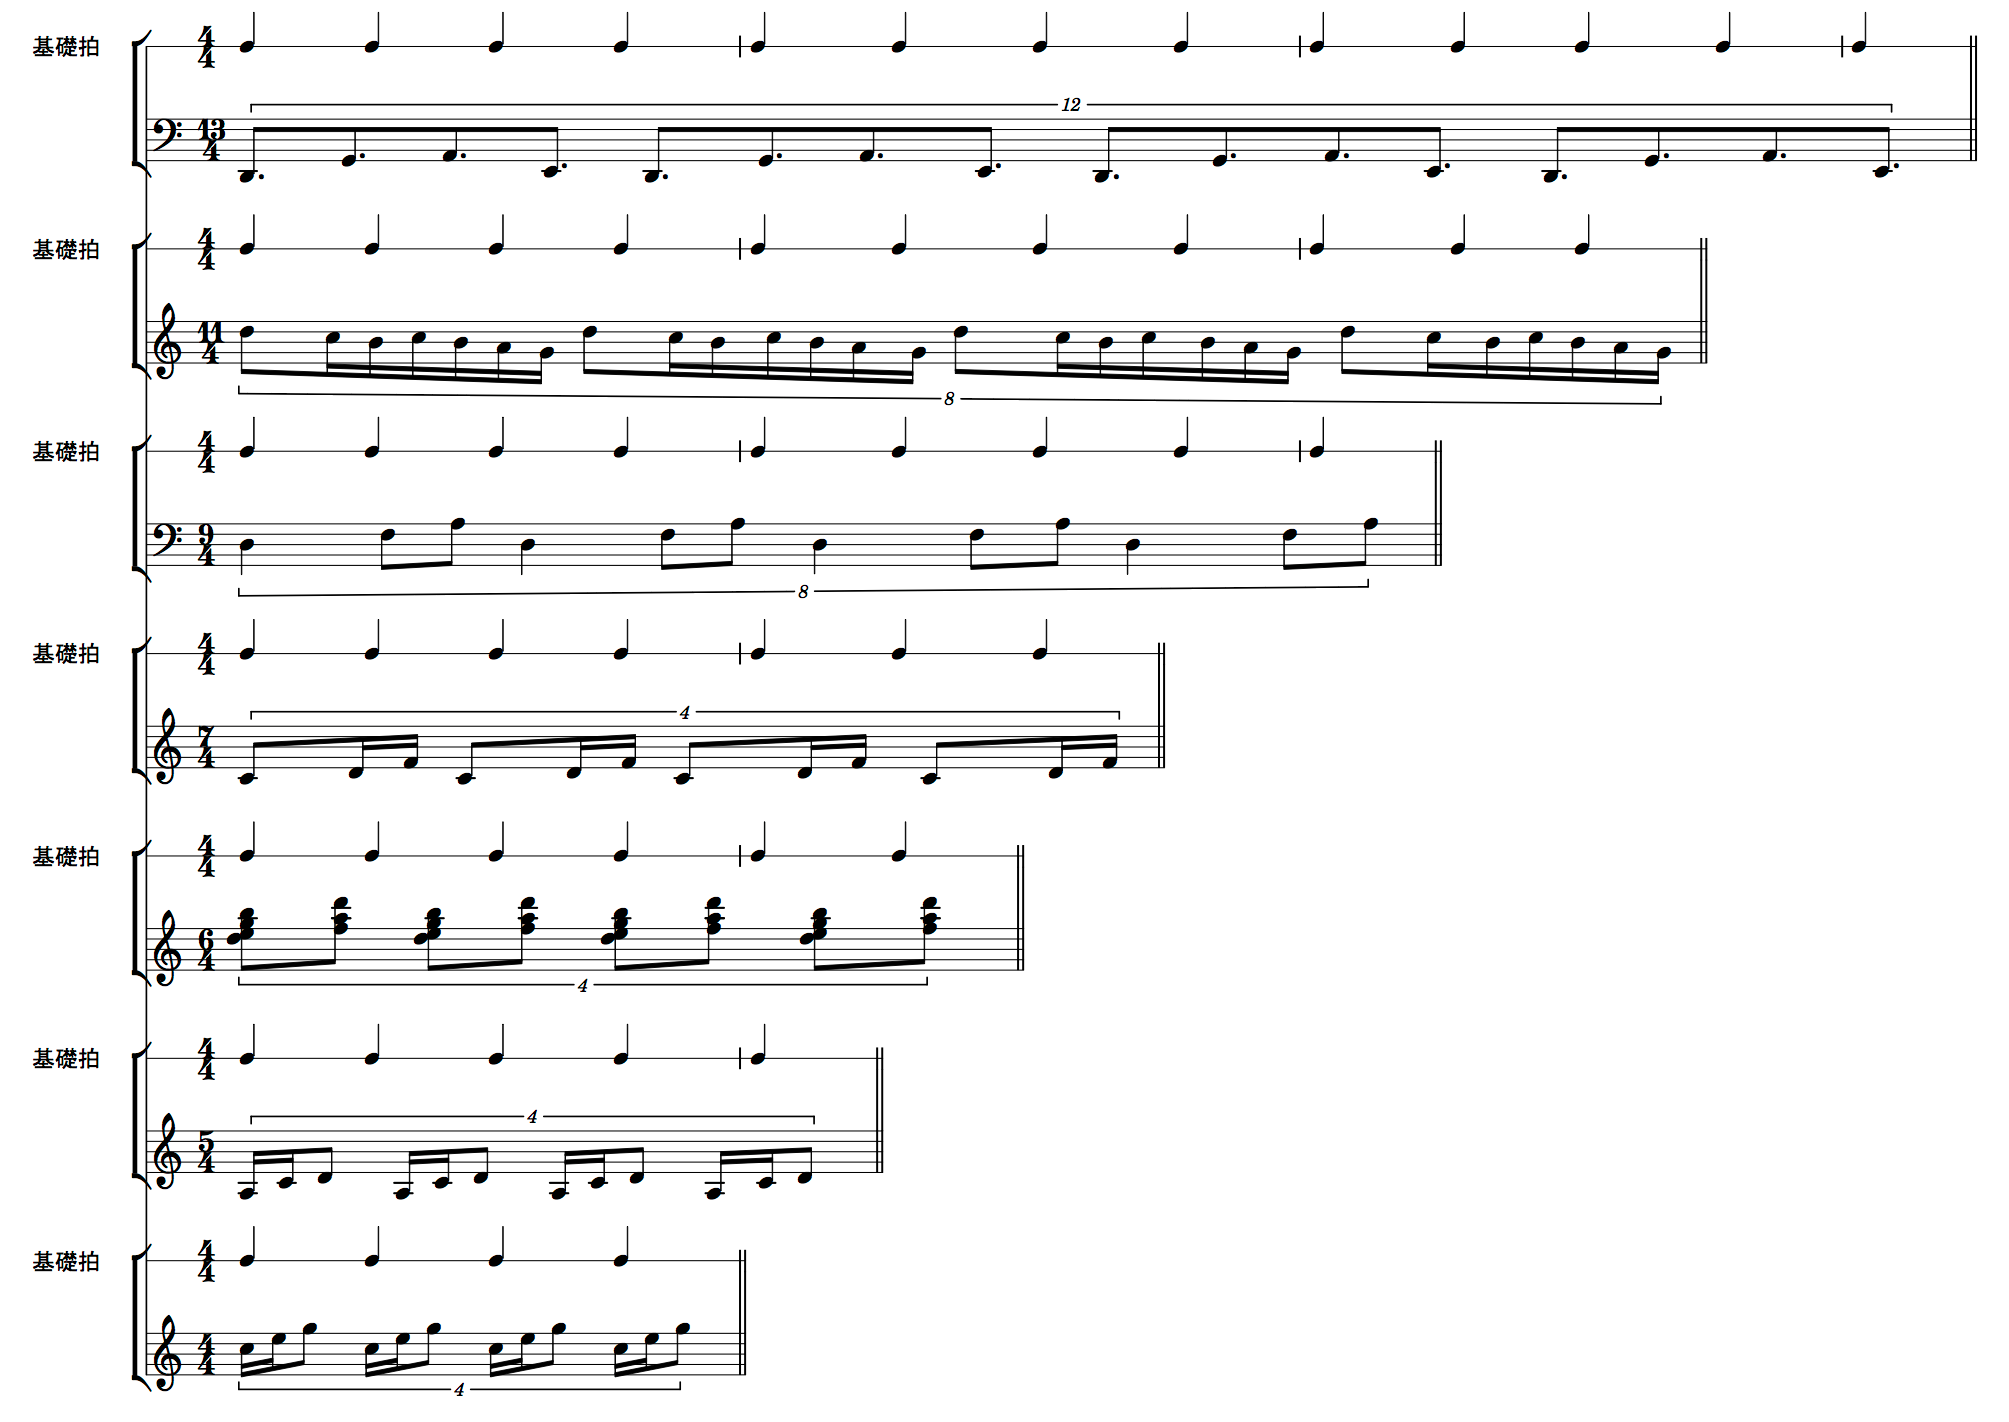
\includegraphics[
 width=\textwidth]{./PDF/figure_26.pdf}
}
\caption{Phrase score of Piano Etude. From top to bottom: 13-beat in 4/4 meter, 11-beat in 4/4 meter, 9-beat in 4/4 meter, 7-beat in 4/4 meter, 6-beat in 4/4 meter, 5-beat in 4/4 meter, 4-beat in 4/4 meter.}
\label{fig:figure_26}
\end{figure}

\begin{figure}[ht]
\centerline{
	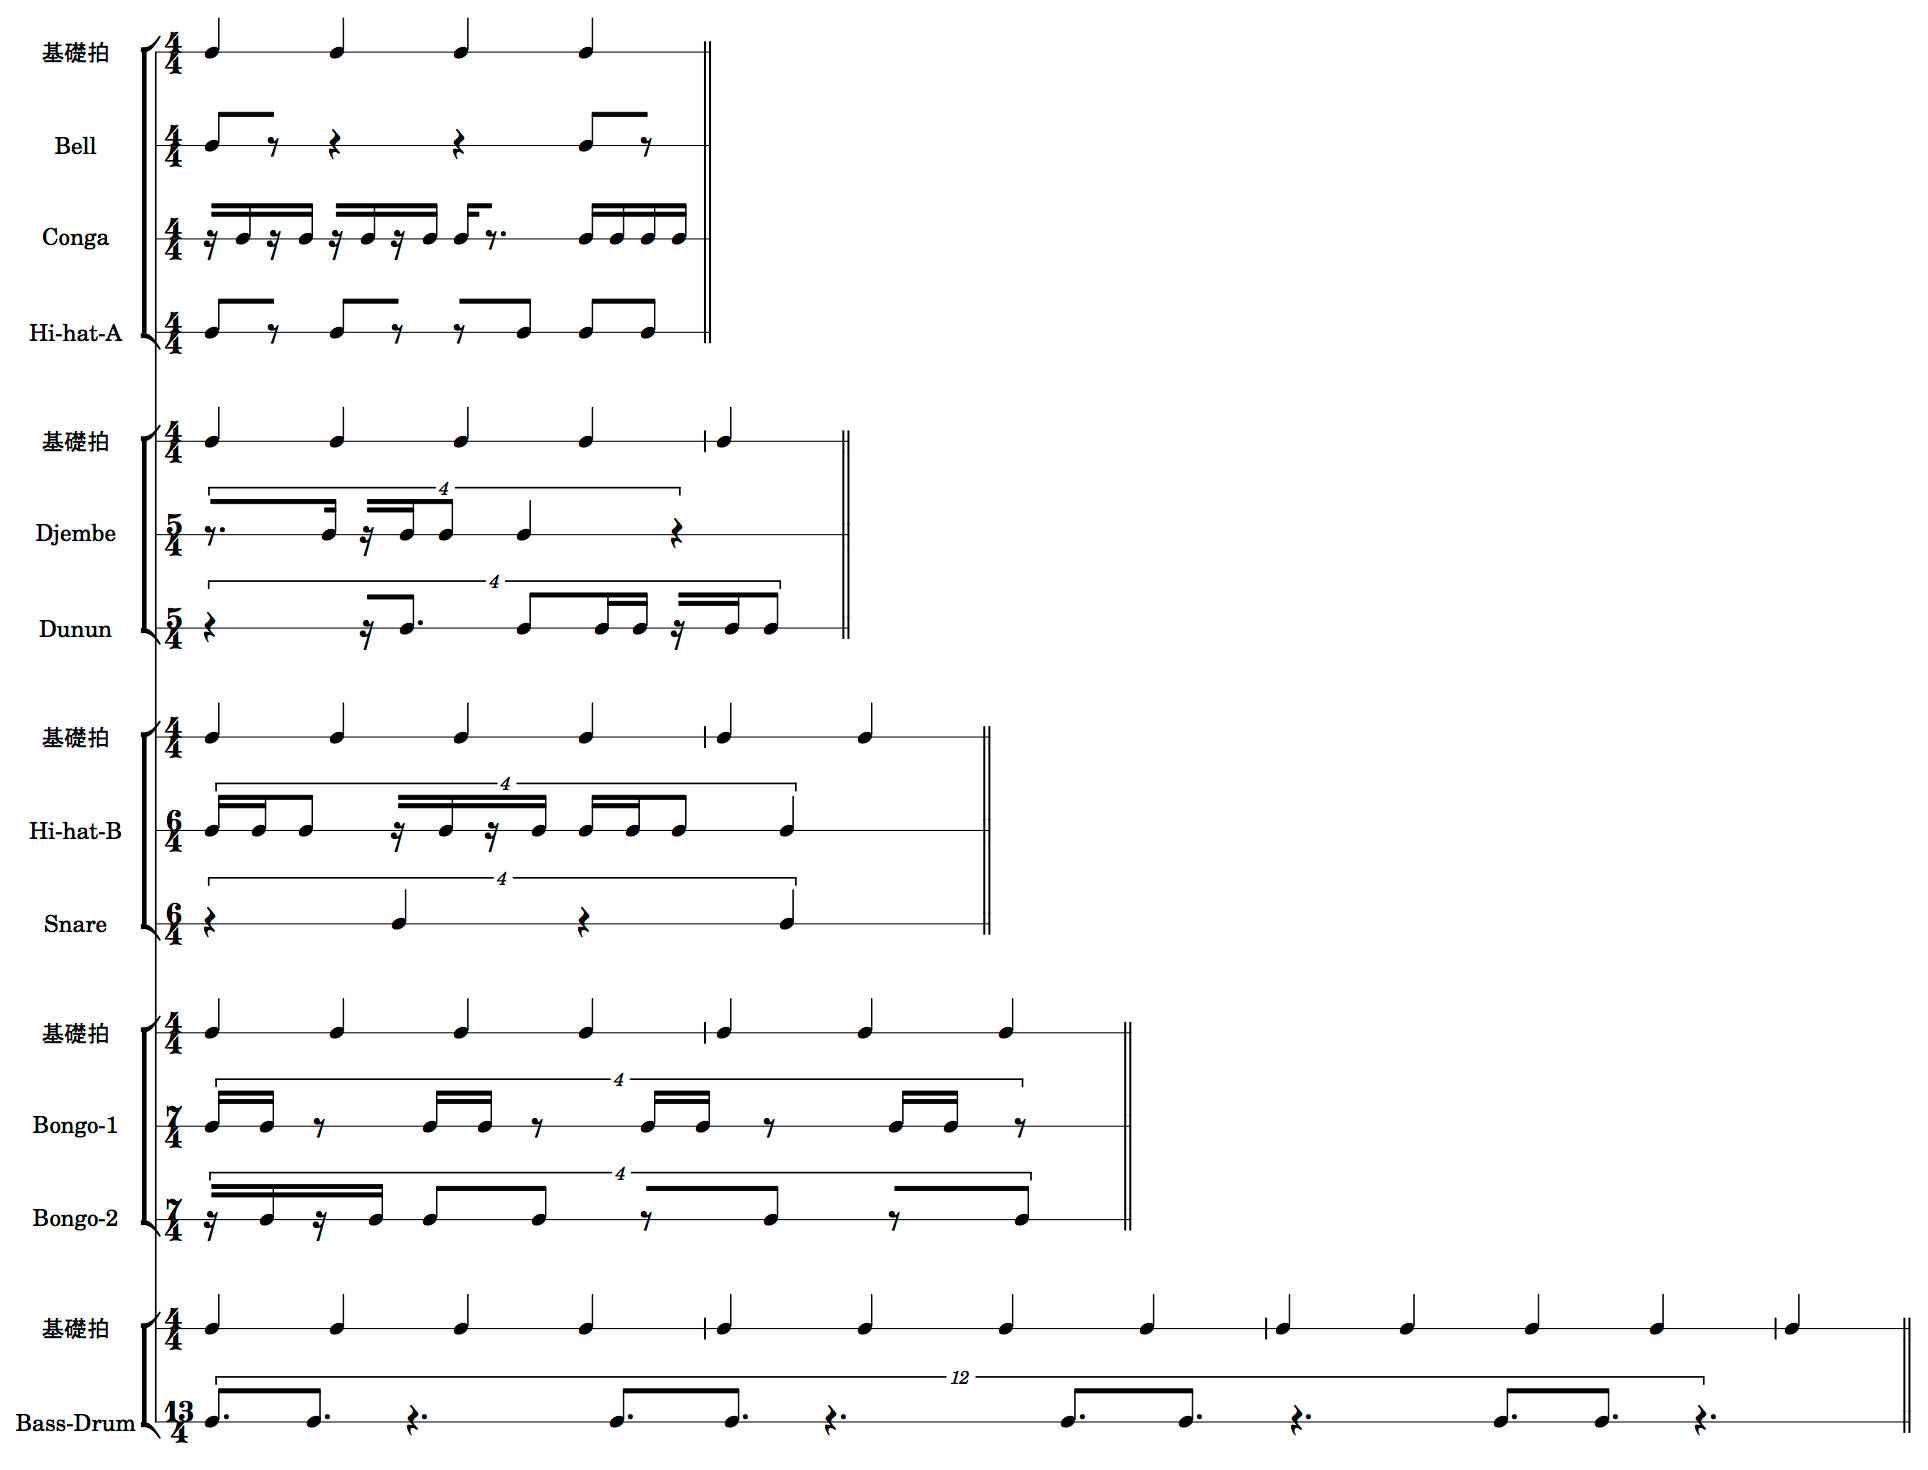
\includegraphics[
 width=\textwidth]{./PDF/figure_27.pdf}
}
\caption{Phrase score of Percussion Ensemble. From top to bottom: 4-beat in 4/4 meter, 5-beat in 4/4 meter, 6-beat in 4/4 meter, 7-beat in 4/4 meter, 13-beat in 4/4 meter.}
\label{fig:figure_27}
\end{figure}

These scores represent each phrase as if written in 4/4 meter, and differ from the actual sounding timings. Figures~\ref{fig:figure_28} (the same can be downloaded from this URL: \url{https://goo.gl/694iHz}) and~\ref{fig:figure_29} (the same can be downloaded from this URL: \url{https://goo.gl/i6J5TM}) show these converted to actual note values.

\begin{figure}[ht]
\centerline{
	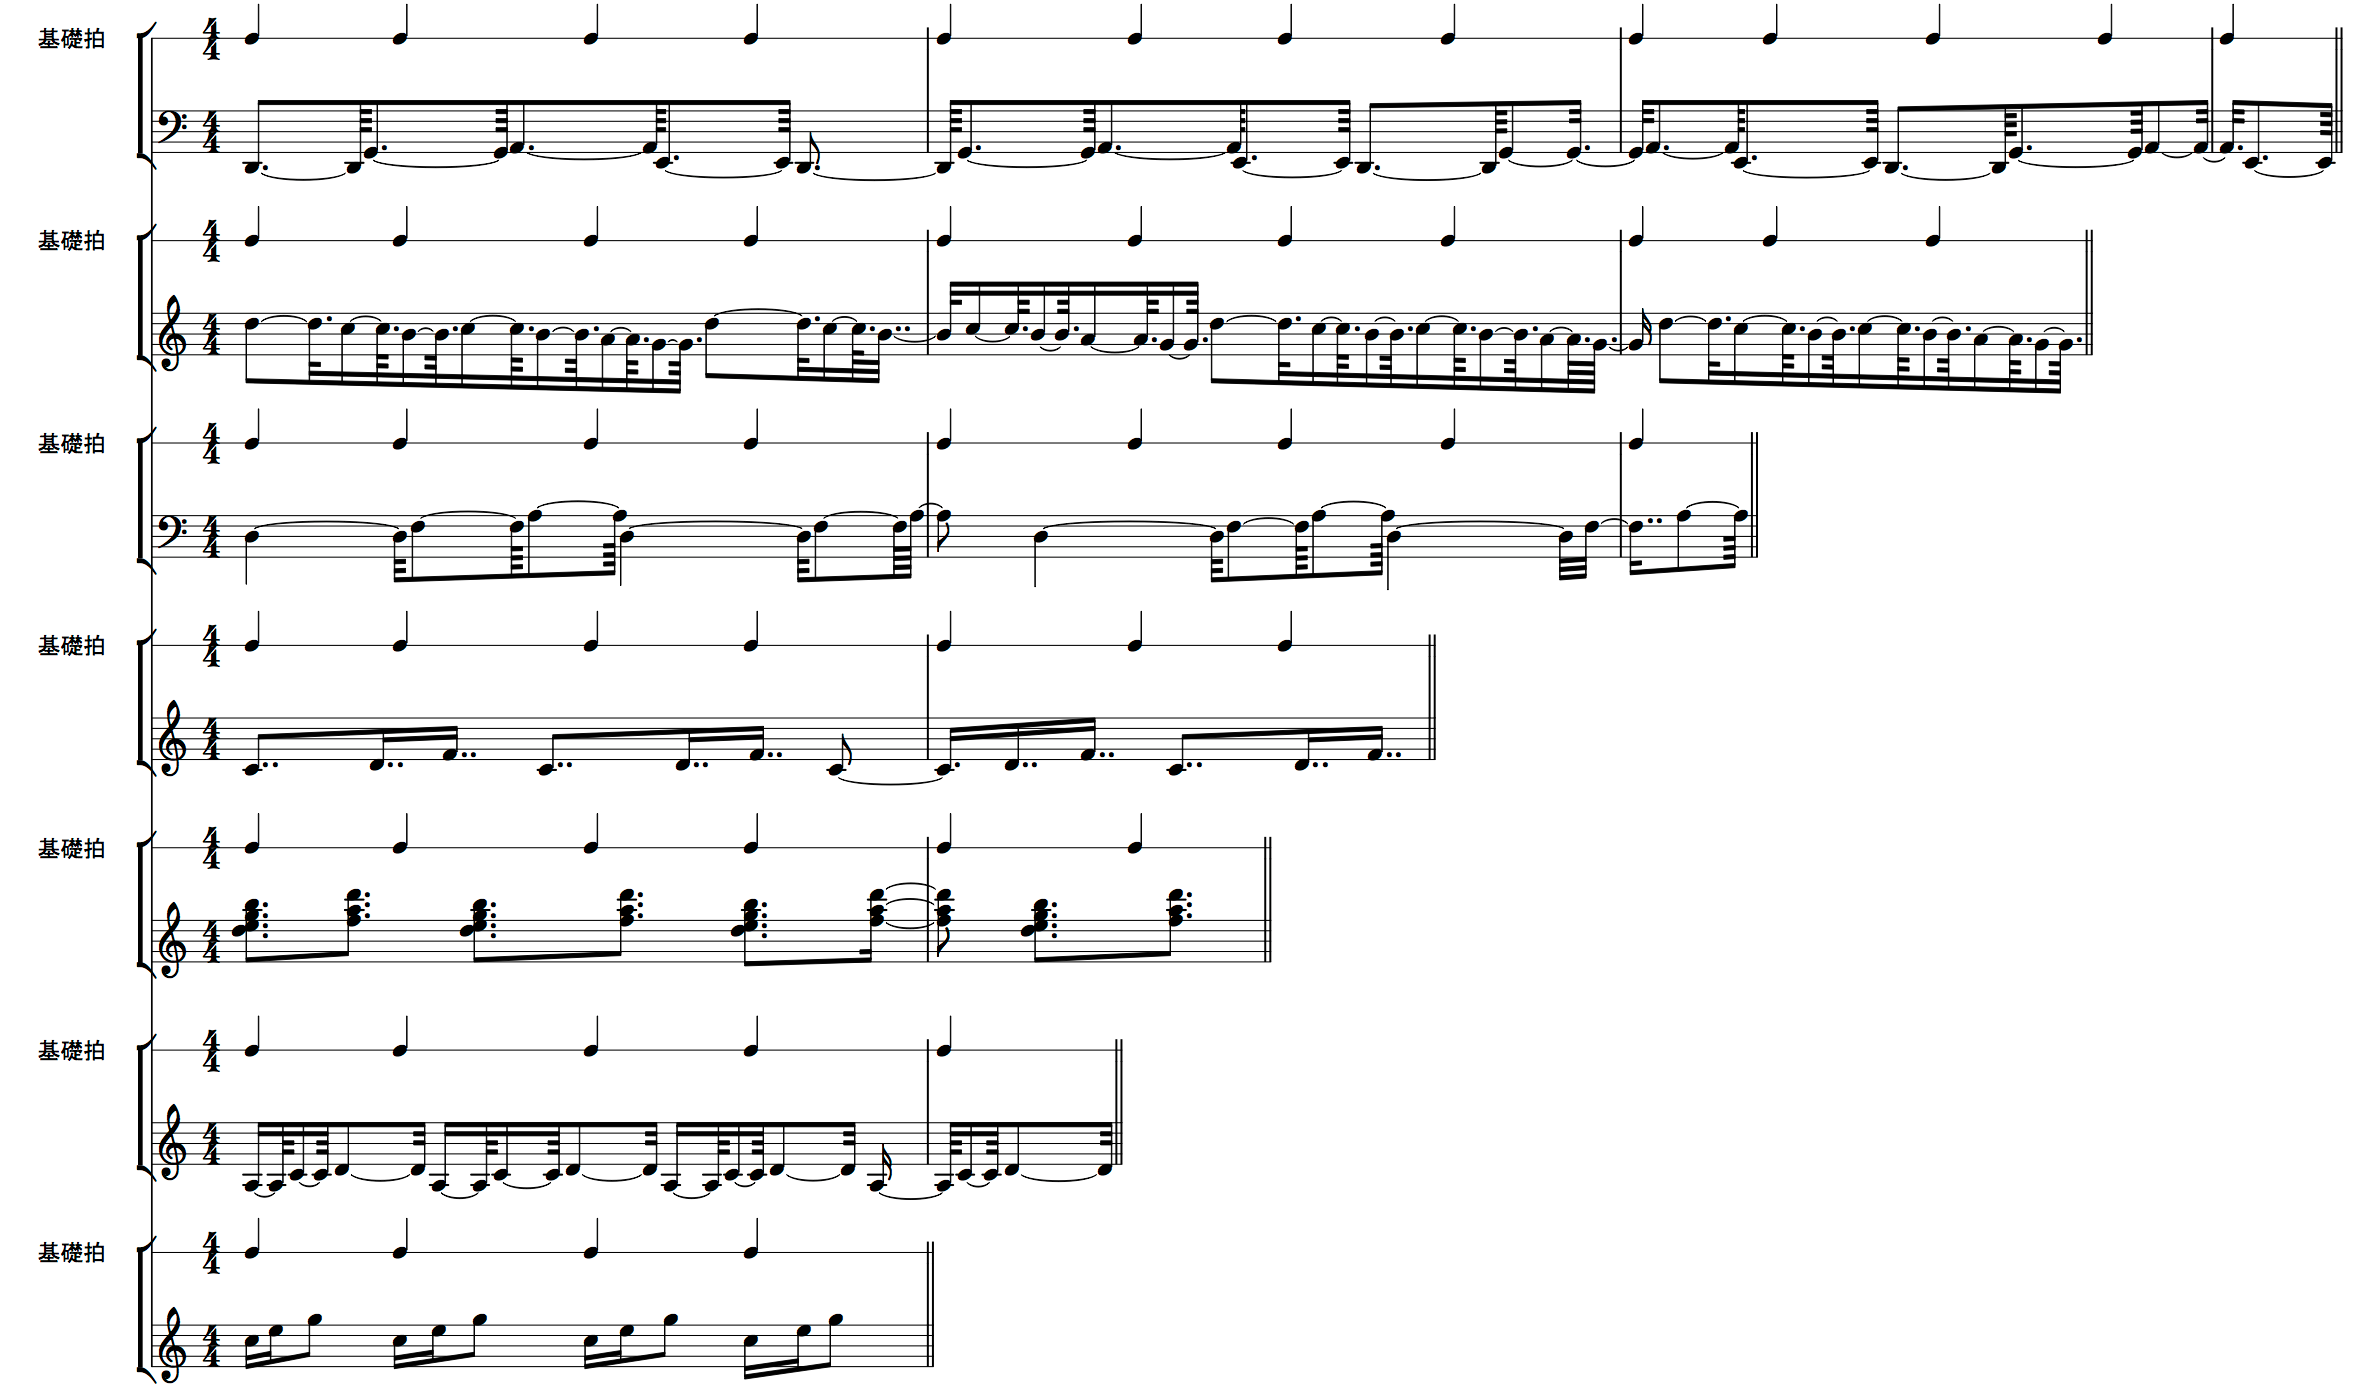
\includegraphics[
 width=\textwidth]{./PDF/figure_28.pdf}
}
\caption{Phrase score of Piano Etude from Figure~\ref{fig:figure_26} converted to actual note values.}
\label{fig:figure_28}
\end{figure}

\begin{figure}[ht]
\centerline{
	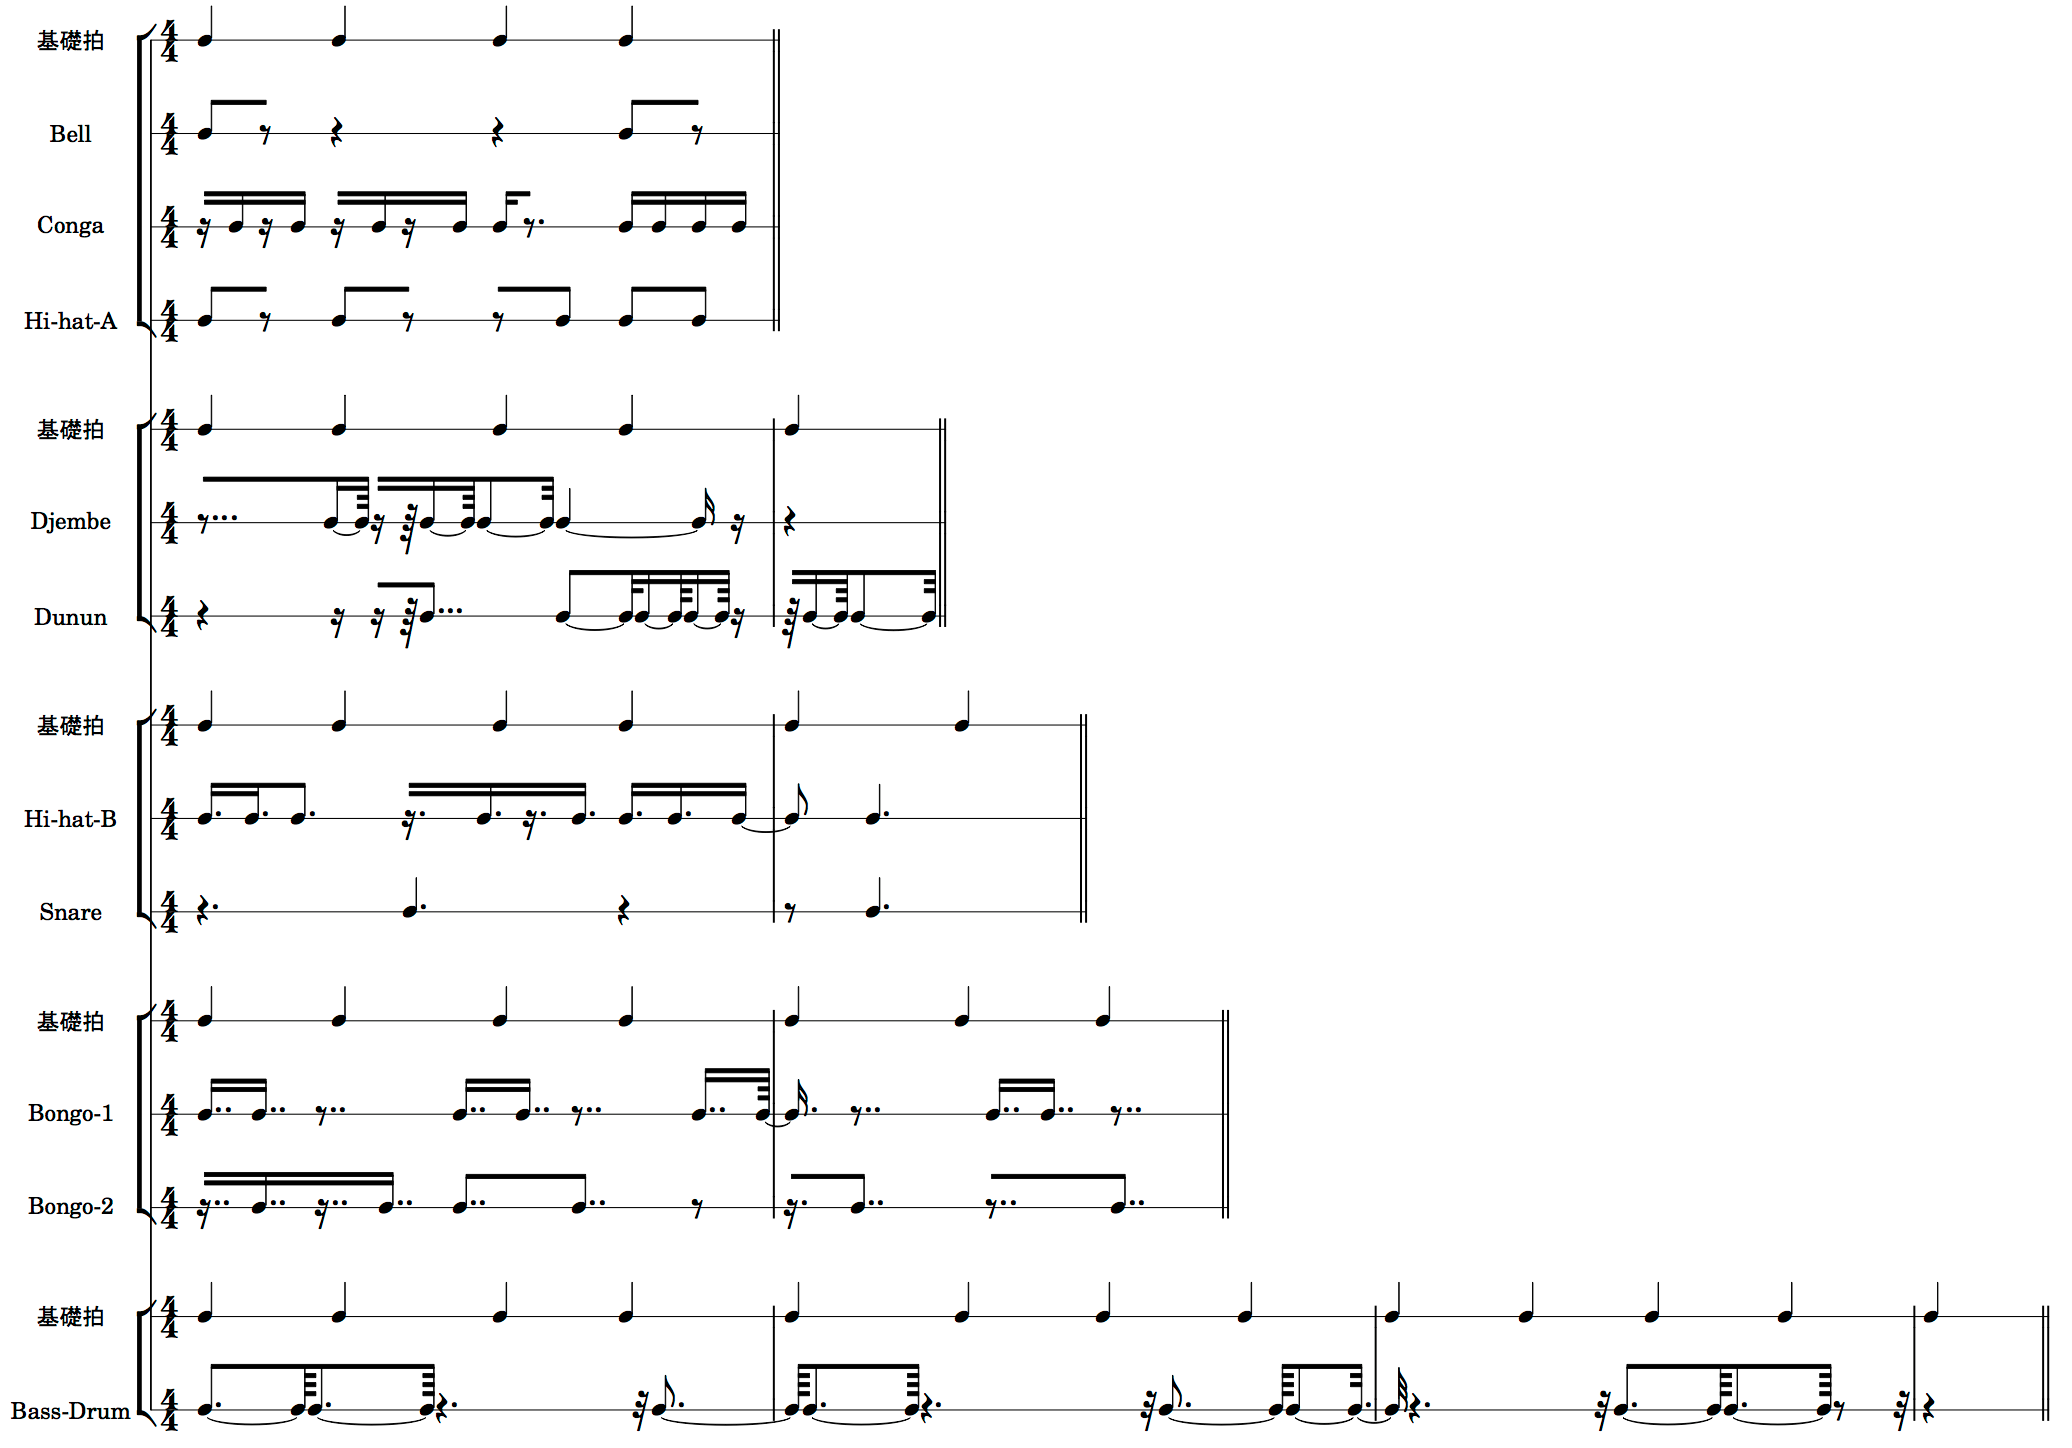
\includegraphics[
 width=\textwidth]{./PDF/figure_29.pdf}
}
\caption{Phrase score of Percussion Ensemble from Figure~\ref{fig:figure_27} converted to actual note values.}
\label{fig:figure_29}
\end{figure}

Through performing division into 4 across bar lines in this way, it became clear that fluctuations and inflections with very fine granularity of note values, which are not seen in conventional musical pieces, can be created through simple rules. It was through these efforts that I conceived what is explained next: "music with multilayered temporal structures."

%改ページや図版を章に収めたい場合は以下のように改ページすると収まる。
\afterpage{\clearpage}
\newpage

\subsection{Definition of "Music with Multilayered Temporal Structures"}

"Music with multilayered temporal structures" is largely defined by the following two elements:

\begin{enumerate}
  \item Lines (melodies, rhythms, instrumental parts) of different tempos flow simultaneously
  \item The lines of different tempos in item 1 "periodically align at the first beat of a certain measure"
\end{enumerate}

To put it simply, it is "music made up of multiple layers of $ n $-beat in 4/4 meter at different BPMs," but unlike so-called random multi-BPM or free tempo, the characteristic feature is that beats align at a certain cycle.

\begin{figure}[ht]
\centerline{
	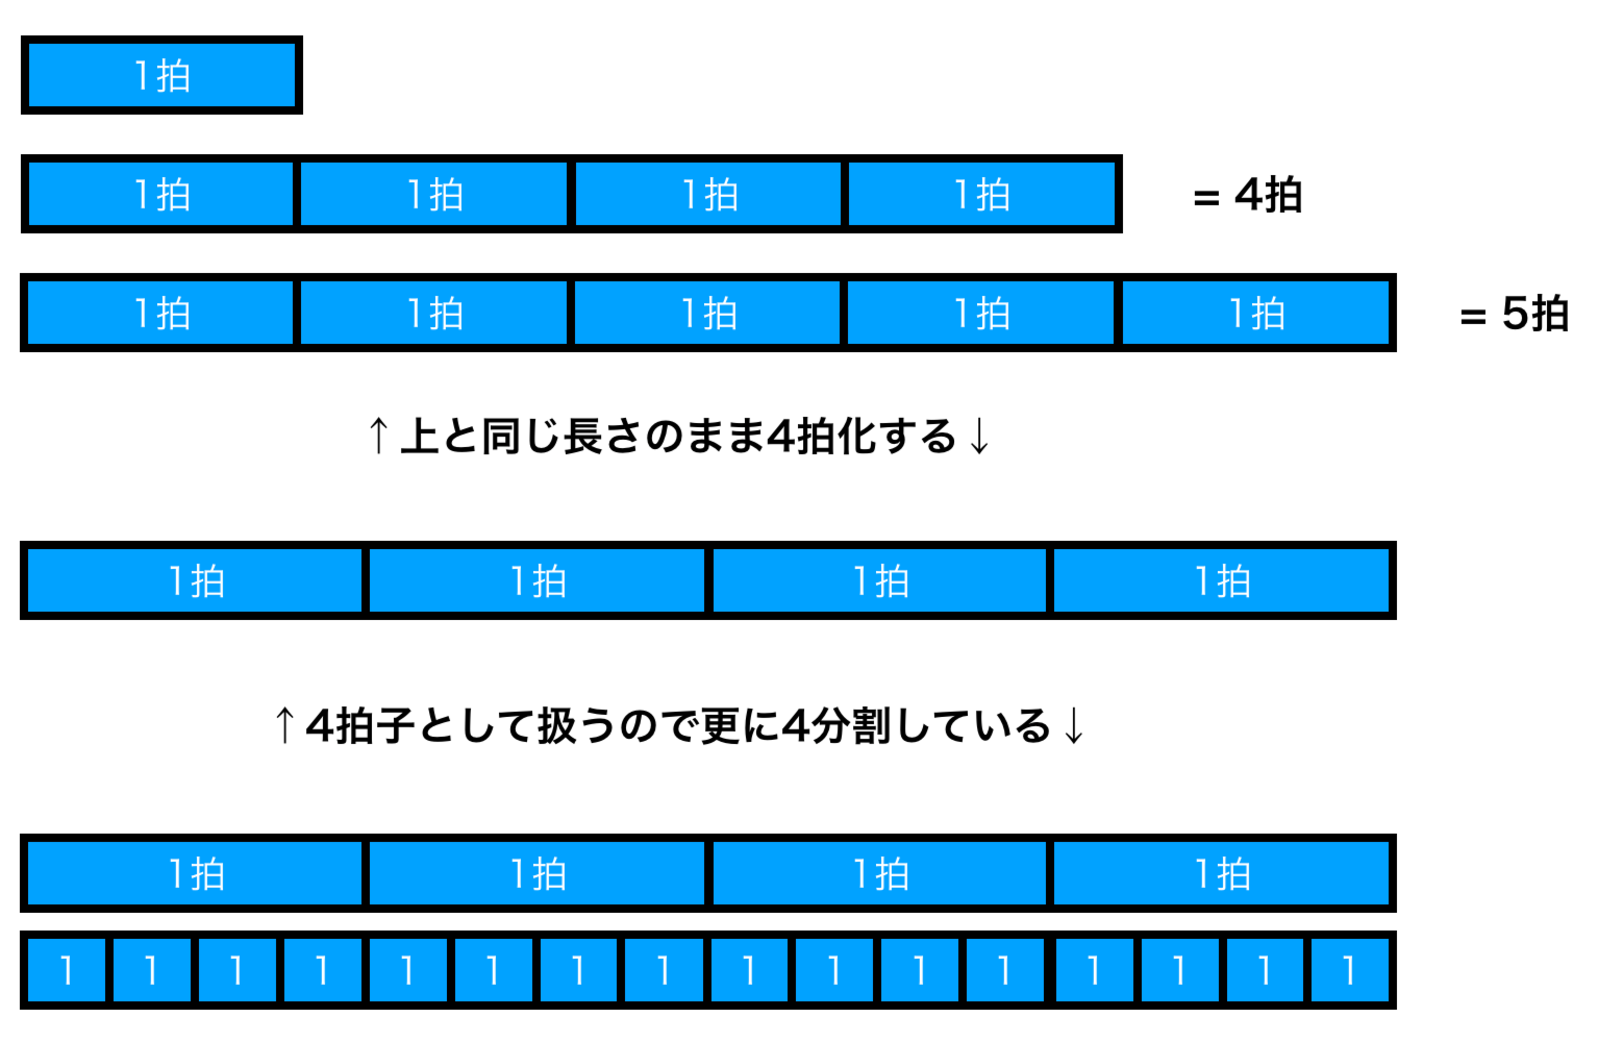
\includegraphics[
 width=\textwidth]{./PDF/figure_01.pdf}
}
\caption{Diagram showing the process of creating 5-beat in 4/4 meter from the common beat of 4-beat in 4/4 meter. By arranging five 1-beat units of 4-beat in 4/4 meter, one can create 5-beat in 5/4 meter. By converting this length as-is into quadruplets, it becomes 5-beat in 4/4 meter. Also, by dividing 1 beat into 4 as the basic grid of 4/4 meter, one can create the 16th note grid for 5-beat in 4/4 meter.}
\label{fig:figure_01}
\end{figure}

Figure~\ref{fig:figure_01} shows the concept of 5-beat in 4/4 meter in the case of multiple layers of 4-beat in 4/4 meter and 5-beat in 4/4 meter. First, based on the length of one beat in 4-beat in 4/4 meter (that is, normal 4/4 meter), take the length of 5 beats. Convert this length as-is into 4 beats (in other words, it becomes synonymous with 5-beat quadruplets). At that time, by treating both as 4/4 meter without sharing bar lines, 4/4 meters with different tempos are layered. Furthermore, since these 4-beat in 4/4 meters originally had lengths of 4 and 5 beats respectively and share the length of one beat, the beat attack points align at the downbeat of the next measure (21st beat) following the 4th beat of the 5th measure corresponding to the 20th beat on the 4-beat in 4/4 meter side, and at the downbeat of the next measure (17th beat) corresponding to the 16th beat on the 5-beat in 4/4 meter side. Although this is a simple least common multiple, the $ n $-beat in 4/4 meters of both sides do not align at the beginning of measures in between, and they cycle while causing a displacement of at least 16th notes.

This simple method of layering $ n $-beat in 4/4 meter is the basic concept of "music with multilayered temporal structures."

\subsection{Notation in "Music with Multilayered Temporal Structures"}
Regarding notation in "music with multilayered temporal structures," as can be seen from the previous prototype examples, conventional notation becomes difficult to read. Therefore, in order to clearly show the composer's subjective view while ensuring readability, I use notation called "variable meter notation" and "fixed meter notation." Below, I will explain each based on the pieces included in the work ''Music for multilayered temporal structures''. Figure~\ref{fig:figure_02} below corresponds to the Drum part of the piece ''Etude \#1'' included in the same work.

\begin{figure*}[htb]
\centerline{
	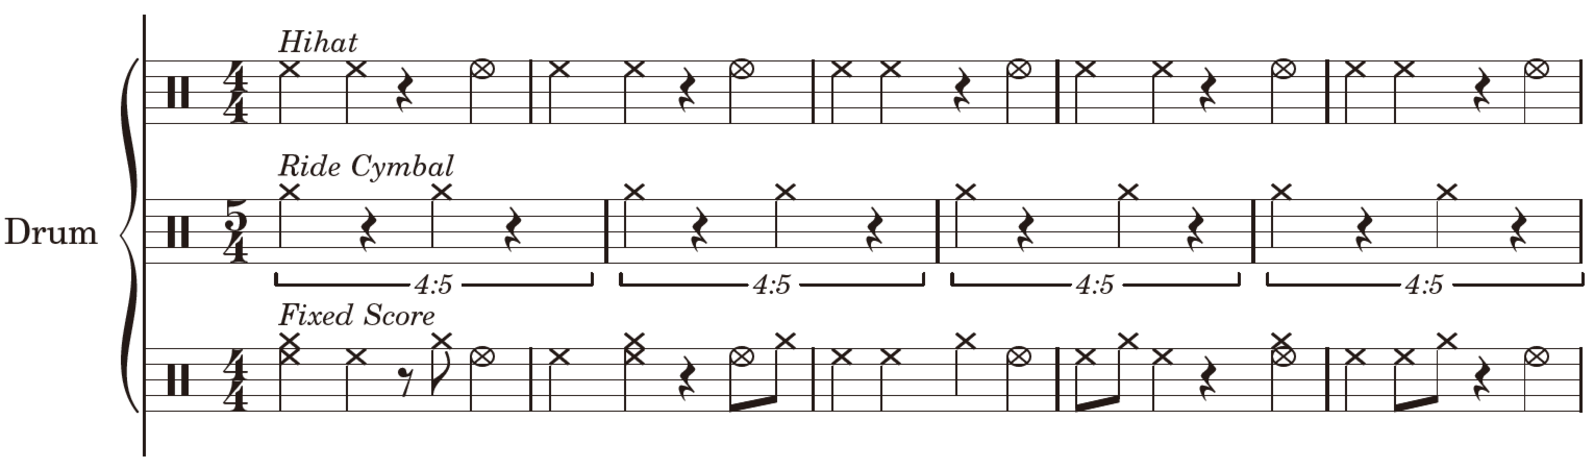
\includegraphics[
 width=\textwidth]{./PDF/figure_02.pdf}
}
\caption{Drum part of Etude \#1 INTRO section}
\label{fig:figure_02}
\end{figure*}

In the score example of Figure~\ref{fig:figure_02}, the top two staves show the "variable meter notation" score of the multiple layers of 4-beat in 4/4 meter and 5-beat in 4/4 meter. The characteristic of variable meter notation is that, in the case of this score, since it becomes multiple layers of $ n $-beat in 4/4 meter, bar lines are not shared between 4-beat in 4/4 meter and 5-beat in 4/4 meter, and the phrases wrap around. Also, although the 5-beat in 4/4 meter side is equivalent to so-called "5-beat quadruplets," with ordinary tuplet note values it is not possible to show the concept of $ n $-beat in 4/4 meter that "bar lines wrap around and the length of the fundamental beat is different," so tuplet symbols are indicated as "4:5" and aligned in notation with the note values of each 4/4 meter.

In contrast, the part indicated as "Fixed Score" in the third staff of the same score example corresponds to "fixed meter notation." This is the "variable meter notation" of the top two staves compiled into a form with aligned bar lines (here, 4-beat in 4/4 meter), and corresponds to what is generally called conventional score format.

Also, in ''Etude \#3'' included in the same work, it is necessary to use notation as shown in Figure~\ref{fig:figure_03}.

\begin{figure*}[htb]
\centerline{
	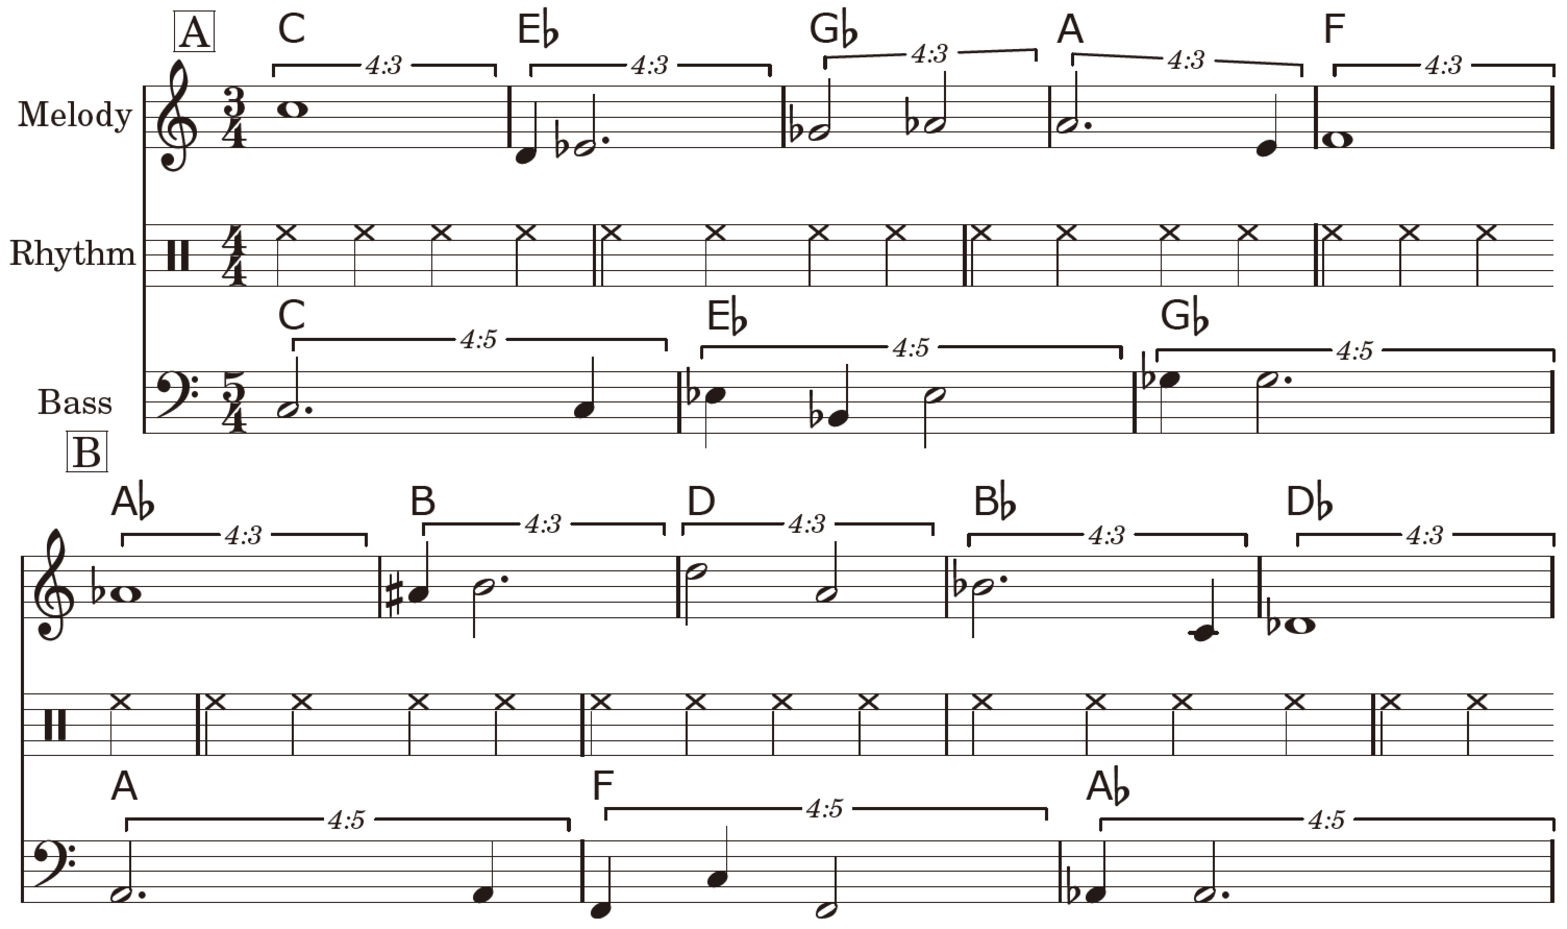
\includegraphics[
 width=\textwidth]{./PDF/figure_03.pdf}
}
\caption{Etude \#3 [A][B] section}
\label{fig:figure_03}
\end{figure*}

''Etude \#3'' is composed in three layers: 3-beat in 4/4 meter, 4-beat in 4/4 meter, and 5-beat in 4/4 meter. This is an example of its "variable meter notation," but 3-beat in 4/4 meter (first staff of the score example) and 5-beat in 4/4 meter (third staff of the score example) align at the end of measures after 5 measures and 3 measures respectively, similar to the previous ''Etude \#1''. In contrast, 4-beat in 4/4 meter (second staff of the score example) needs to wrap to the next line in the middle of a bar line.

In this way, notation that would normally be treated as a taboo in reading conventional score formats becomes necessary, which is one characteristic of music with "multilayered temporal structures," and this raises awareness of problems with the score as a "system that guarantees performability" and "the environment itself related to music production," while simultaneously connecting to "new musical experiential characteristics with diversity" born from rhythm.

\subsection{Rhythm in "Music with Multilayered Temporal Structures"}

Next, I will explain rhythm in "music with multilayered temporal structures."

First, as mentioned earlier, the basic cycle of rhythm in "music with multilayered temporal structures" is the multiple layers of "$ n $-beat," meaning in the case of layers of 4-beat and 5-beat units like "Etude \#1" and "Etude \#2," it can be considered a cycle with 20 as the least common multiple. Just as the 3:4 rhythm of Africa mentioned earlier can be shown as 12/8 meter divided into 3+3+3+3 and 4+4+4 respectively, in the case of a 4:5 rhythm, if converted to one measure, it becomes 20/16 meter, which takes the form of vertical hemiola with 4+4+4+4+4 and 5+5+5+5 respectively, and this has fundamentally the same structure as basic African polyrhythm (cross-rhythm in the definition of this paper). Even with 3:4:5 in "Etude \#3," although the least common multiple is 60 and the cycle at which phrase wraparound aligns becomes larger compared to 4:5, it remains vertical hemiola as is. In order to generate polyrhythmic fluctuation from this vertical hemiola, each $ n $-beat was converted into 4/4 meter.

The specific method for calculating beat attack points is as follows. The beat $ N $ at which "multiple layers of $ n $-beat in 4/4 meter with polyrhythmic fluctuation align at the downbeat point of the measure" is the beat obtained by adding 1 to the least common multiple $ LCM $ of each $ n $-beat. Next, by dividing the least common multiple $ LCM $ by $ n $-beat, the number of measures $ bars $ can be calculated. Furthermore, by multiplying the number of measures $ bars $ by 4, the number of quarter notes $ beats $ until each $ n $-beat in 4/4 meter aligns at the downbeat can be determined (multiplying by 8 gives the number of eighth notes). The above can be shown by the following simple formula:\\

\begin{math}
beats = LCM \div n \times 4
\end{math}\\

By dividing $ LCM $ by the obtained $ beats $, the length of one beat $ length $ for each $ n $-beat in 4/4 meter can be calculated.\\

\begin{math}
length = LCM \div beats
\end{math}\\

By multiplying this by values from 1 to the maximum value $ m $ of $ beats $, the position of each beat $ p $ can be calculated from $ LCM $.\\

\begin{math}
(p_1,p_2\dots,p_m) = length \times (beats_1,beats_2\dots,beats_m)
\end{math}\\

By relativizing these values and comparing each $ n $-beat in 4/4 meter, the common beats of each $ n $-beat in 4/4 meter can be determined. For actual comparison, I initially used hand calculations on graph paper, and later used a program implemented on openFrameworks. The common beat attack points obtained from this comparison are used as rhythmic motifs in the composition. The programs used, ''4by5''\cite{yamato:02} and ''3by4by5''\cite{yamato:03}, are published in the author's GitHub repository.

Also, as mentioned earlier, the concept of multiple layers of $ n $-beat in 4/4 meter can be called multiple layers of "4/4 meter at different BPMs." In this case, each $ BPM $ can be calculated by the following formula when the basic BPM is $ BaseBPM $:\\

\begin{math}
BPM = BaseBPM \div ( n \div 4 )
\end{math}\\

For example, in the case of ''Etude \#1'', the speed of the basic 4/4 meter is specified as 115 BPM. When applied to the above formula, while 4-beat in 4/4 meter is 115 BPM, 5-beat in 4/4 meter is $ 115 \div ( 5 \div 4 ) = 92 $, or 92 BPM, and it can be seen that it is multiple layers of BPMs in integer ratio 5:4. However, when calculating the BPM of 3-beat in 4/4 meter against this 115 BPM 4-beat in 4/4 meter, it becomes $ 115 \div ( 3 \div 4 ) = 153.333\dots $, and the multiple layers of BPMs can no longer be captured in integer ratios. If the basic BPM is something like 120, all integer ratios can be created, but depending on the basic BPM, it does not become an integer ratio. From this as well, it can be understood that this method can create rhythmic beat attack points with polyrhythmic characteristics that cannot be processed by simple BPM conversion when using programs, etc., using simple rules.

Next, as concrete examples of rhythmic beat attack points, Figure~\ref{fig:figure_04} shows the rhythmic motifs used in "4-beat in 4/4 meter" and "5-beat in 4/4 meter" of ''Etude \#1'' and ''Etude \#2''. In ''Etude \#1'' and ''Etude \#2'', the rhythmic motifs use common beats compared in eighth notes. The green indicates the common beat attack points, but if only those beats were used, the groove of the 4-beat in 4/4 meter side would be lost, so the downbeats of 4-beat in 4/4 meter are also added to the rhythmic motif to express the multiple layers of 4-beat in 4/4 meter and 5-beat in 4/4 meter. Also, Figure~\ref{fig:figure_05} shows this beat attack point notated in "variable meter notation."

\begin{figure*}[htb]
\centerline{
	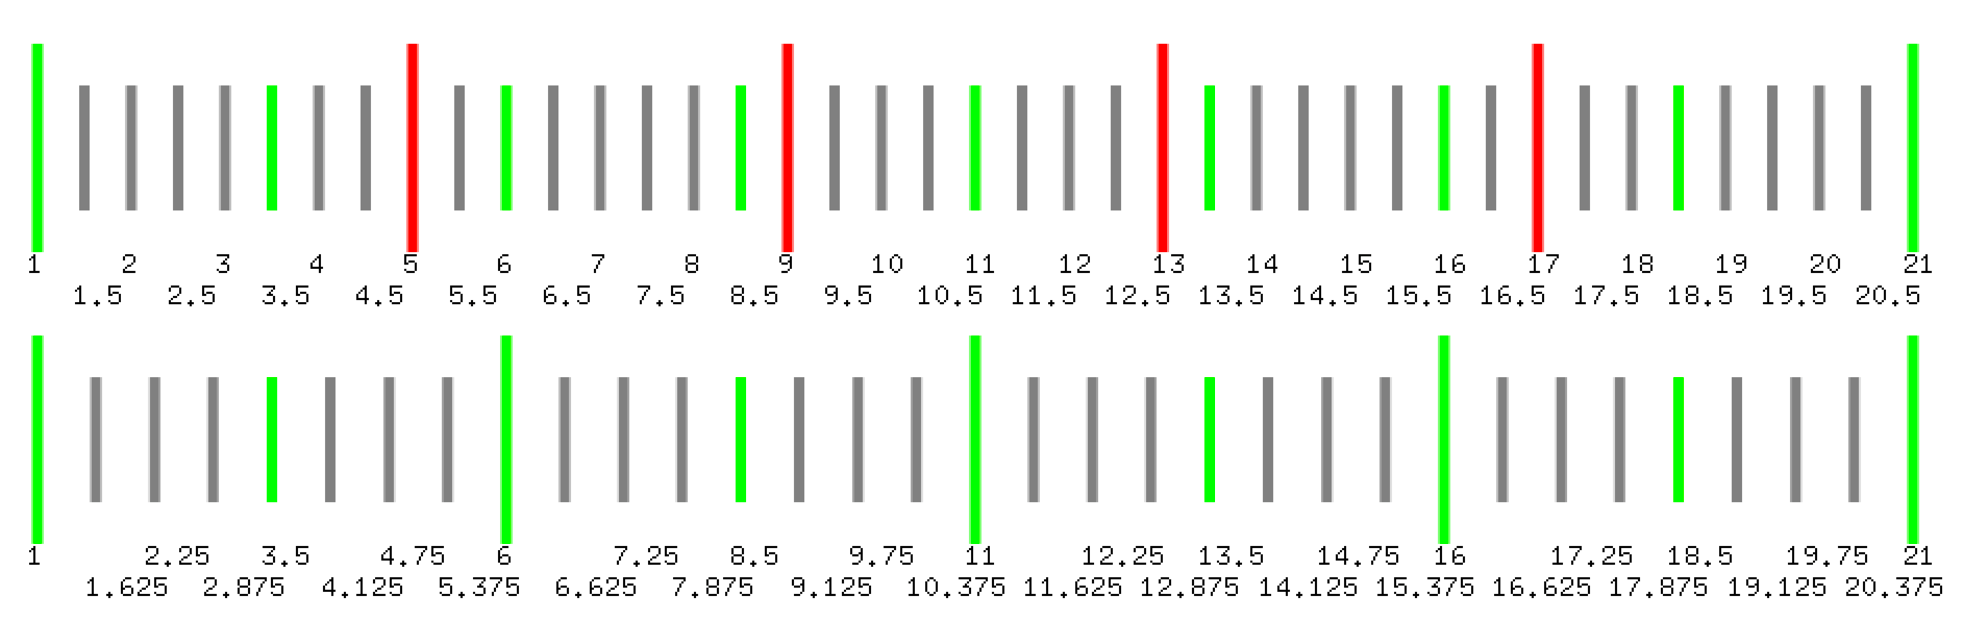
\includegraphics[
 width=\textwidth]{./PDF/figure_04.pdf}
}
\caption{Rhythmic motif diagram of ''Etude \#1'' and ''Etude \#2''. The top of the figure shows the eighth note beat attack points of 4-beat in 4/4 meter. The bottom shows the eighth note beat attack points of 5-beat in 4/4 meter. The green lines indicate the common beat attack points of each. The red lines indicate beat attack points arbitrarily added as rhythmic motifs. The numbers written below the lines numerically indicate the position of each beat attack point.}
\label{fig:figure_04}
\end{figure*}

\begin{figure*}[htb]
\centerline{
	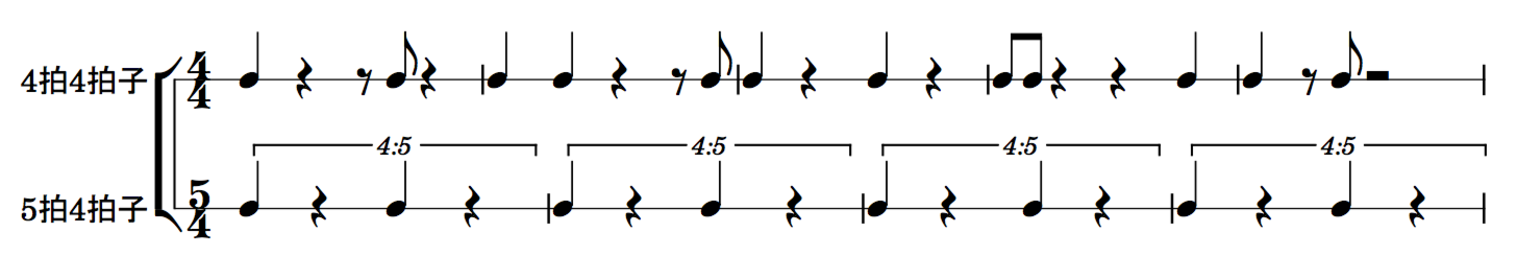
\includegraphics[
 width=\textwidth]{./PDF/figure_05.pdf}
}
\caption{Example showing Figure~\ref{fig:figure_04} in variable meter notation}
\label{fig:figure_05}
\end{figure*}

Next, Figure~\ref{fig:figure_06} shows the rhythmic motif diagram used in the three-layer piece "3-beat in 4/4 meter," "4-beat in 4/4 meter," and "5-beat in 4/4 meter" in ''Etude \#3''. In the actual piece, "4-beat in 4/4 meter" intentionally does not use common beat attack points for compositional purposes.

\begin{figure*}[htb]
\centerline{
	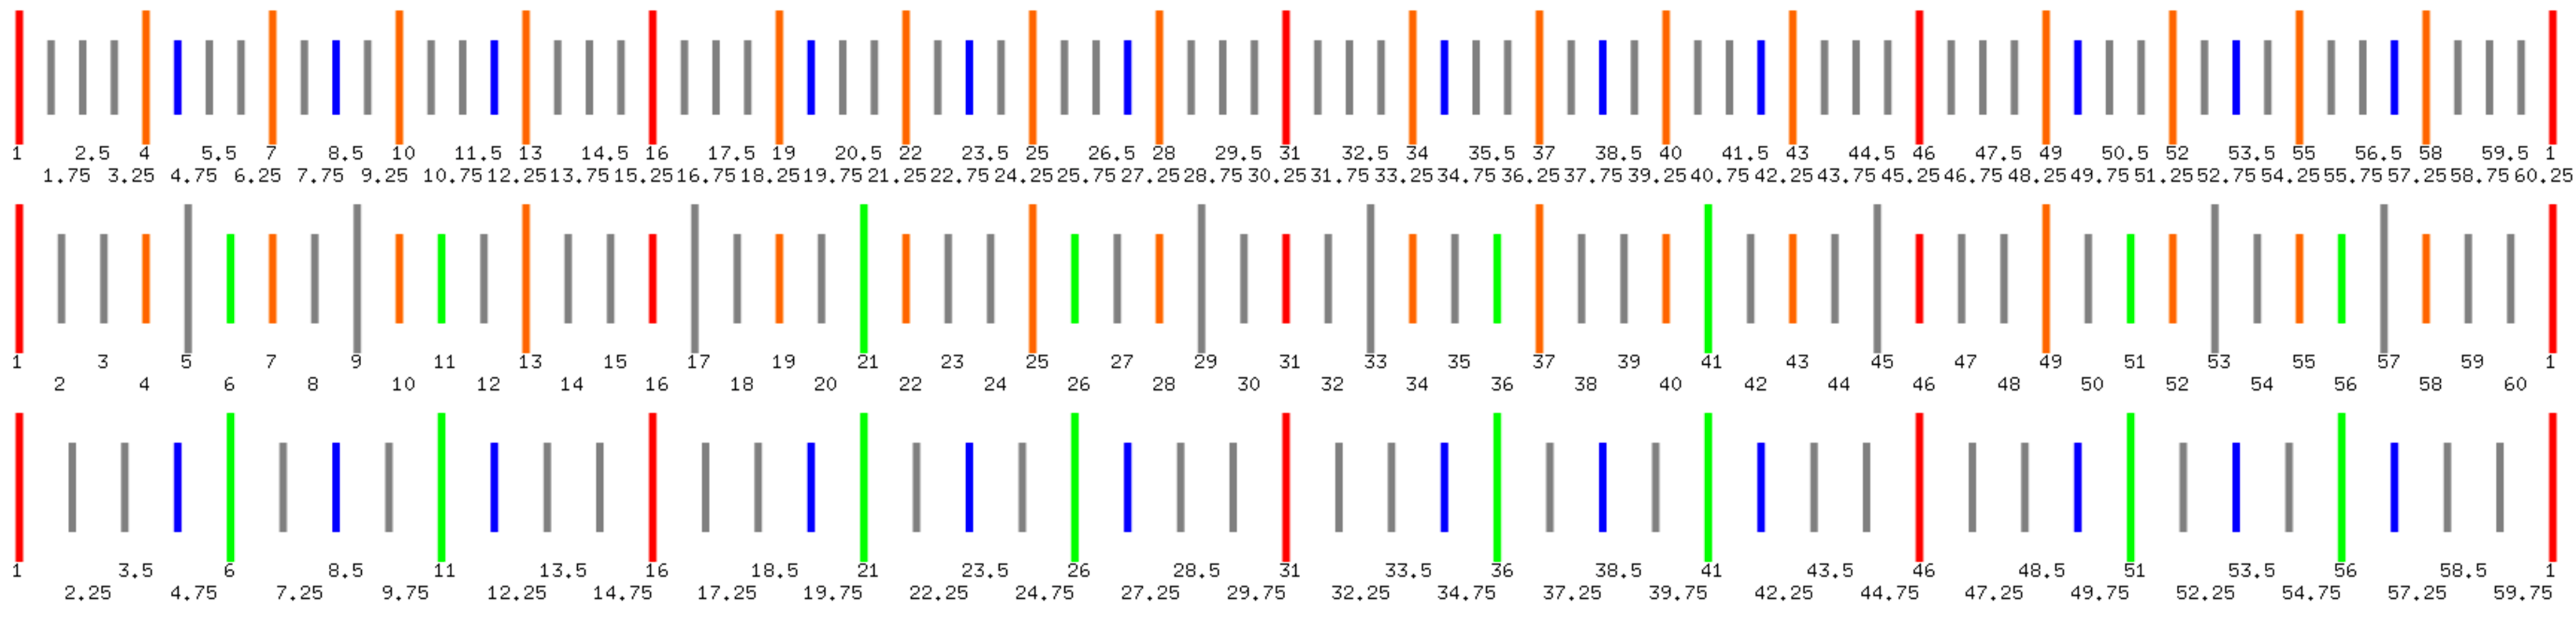
\includegraphics[
 width=\textwidth]{./PDF/figure_06.pdf}
}
\caption{Rhythmic motif diagram of ''Etude \#3''. From top to bottom, showing the beat attack points in quarter notes for 3-beat in 4/4 meter, 4-beat in 4/4 meter, and 5-beat in 4/4 meter. Red indicates beat attack points common to all three meters, orange indicates beat attack points common to 3-beat in 4/4 meter and 4-beat in 4/4 meter, green indicates beat attack points common to 4-beat in 4/4 meter and 5-beat in 4/4 meter, and blue indicates beat attack points common to 3-beat in 4/4 meter and 5-beat in 4/4 meter. Although not visible in the figure display, the numerically expressed position of each beat attack point is shown below each beat attack point, as in Figure~\ref{fig:figure_04}.}
\label{fig:figure_06}
\end{figure*}

This method of using common beats as rhythmic motifs creates relationships between each $ n $-beat in 4/4 meter, making it possible to achieve structural understanding when performing, and each performer can generate the pulse of their respective rhythm themselves. Figure~\ref{fig:figure_07} shows an explanation of "how to take beat attack points" for achieving "structural understanding of rhythm in variable meter notation" explained in the work ''Music for multilayered temporal structures''.

\begin{figure*}[htb]
\centerline{
	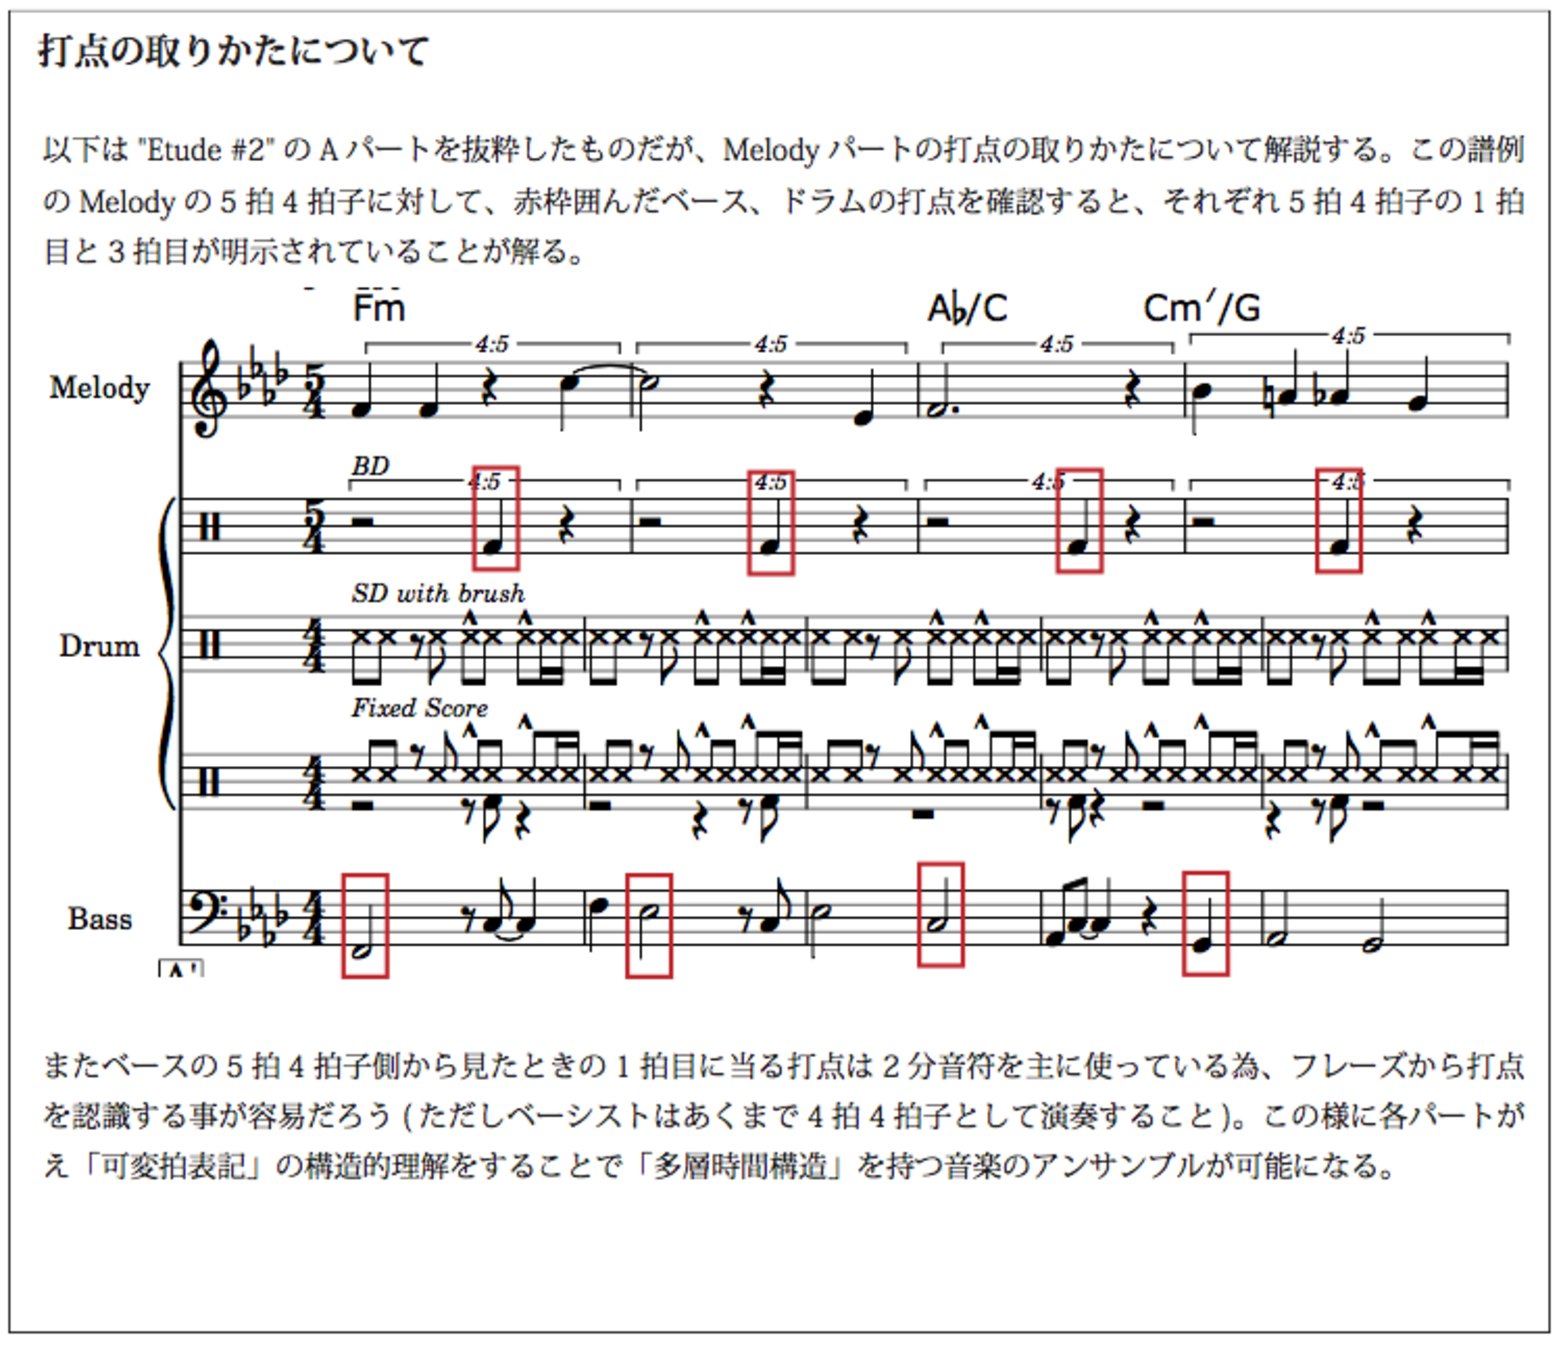
\includegraphics[
 width=\textwidth]{./PDF/figure_07.pdf}
}
\caption{''Etude \#2'' "How to take beat attack points"}
\label{fig:figure_07}
\end{figure*}

As shown in this figure, it becomes possible to generate the tempo of one's own beat from the relationships of common beats, and to read the "variable meter notation" on the time axis.

%改ページや図版を章に収めたい場合は以下のように改ページすると収まる。
\afterpage{\clearpage}
\newpage

\section{Composition "Music for multilayered temporal structures"}

This composition consists primarily of two components: "Etudes" composed using the aforementioned "music for multilayered temporal structures" method, and "performance instructions" for playing these pieces. The compositions here are notated in the so-called "lead sheet" format. Figure \ref{fig:figure_09} shows the lead sheet for "All the Things You Are" from "The Real Book 5th Edition."

\begin{figure}[H]
\centerline{
	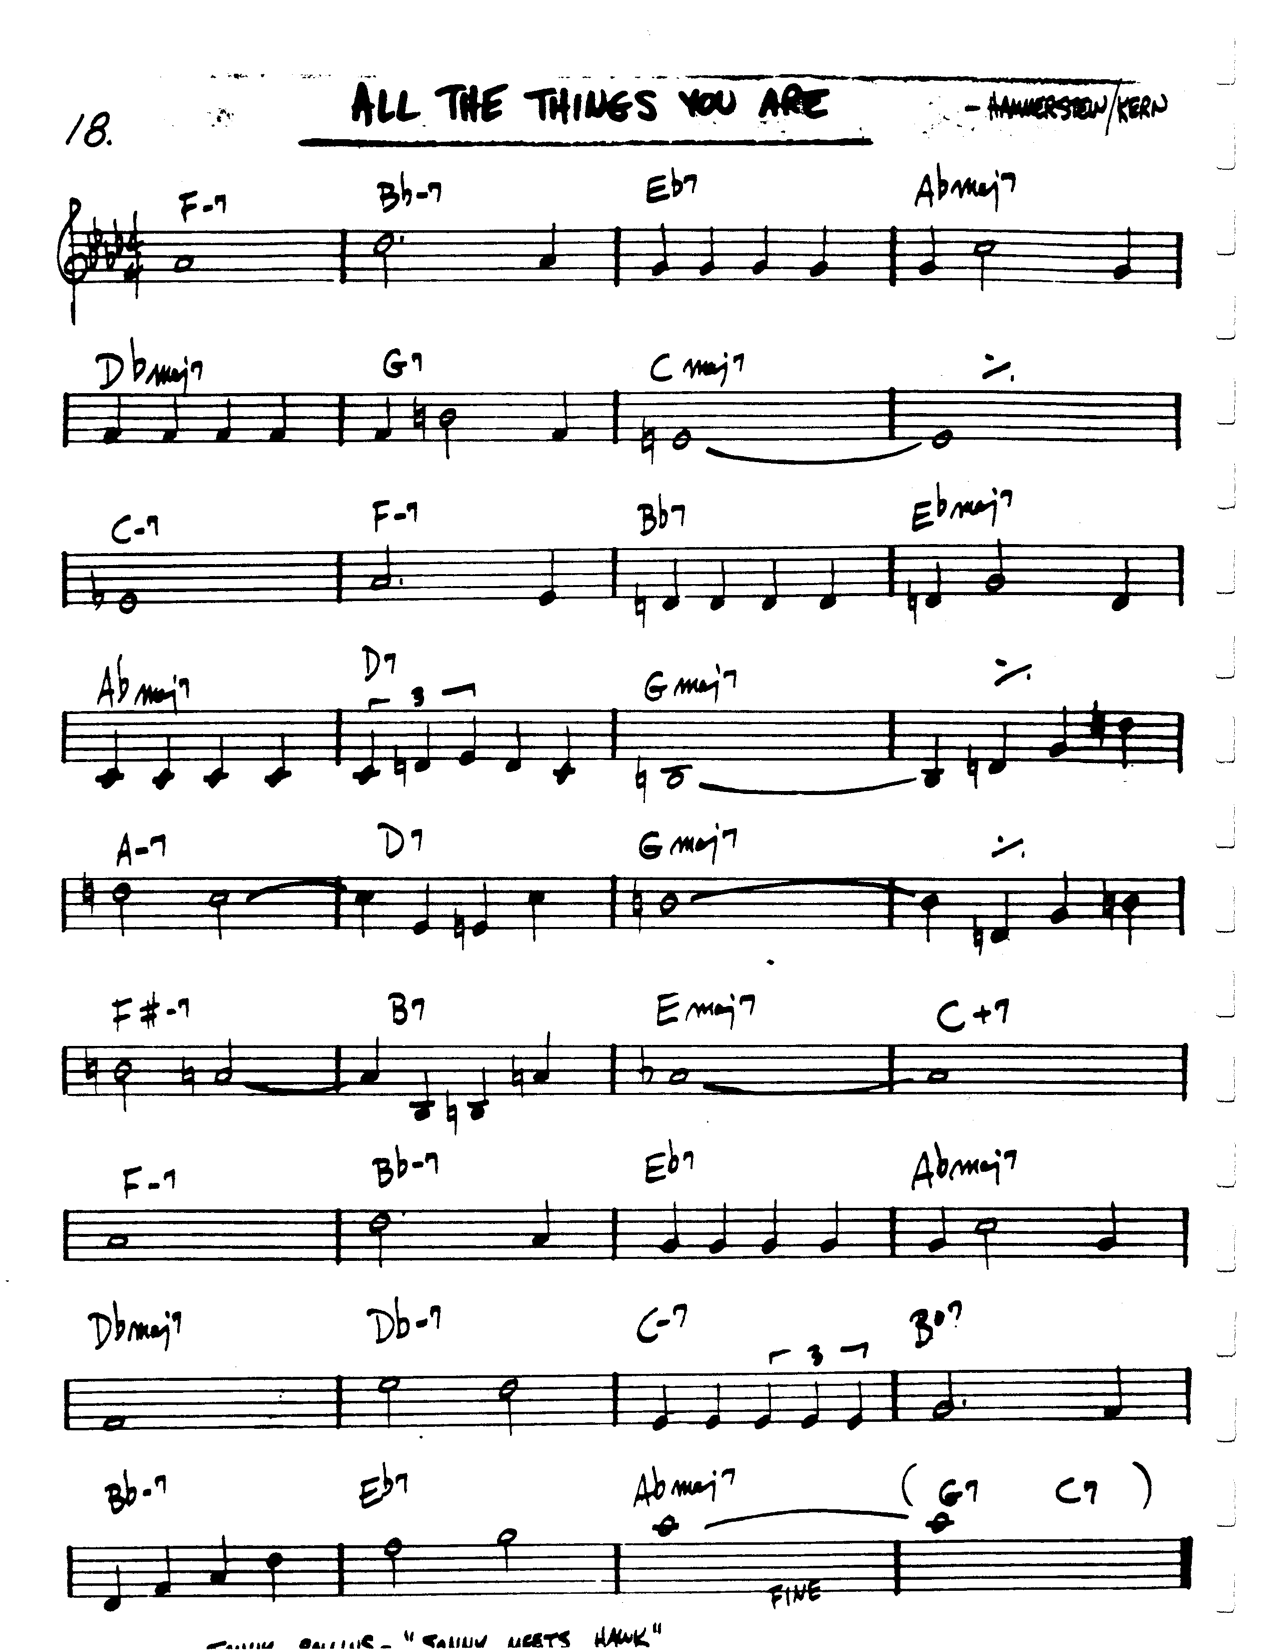
\includegraphics[
 width=0.5\textwidth]{./PDF/figure_09.pdf}
}
\caption{"All the Things You Are" lead sheet}
\label{fig:figure_09}
\end{figure}

Such lead sheets are meta-descriptive musical scores that indicate the structure of a piece through elements such as "key," "time signature," "melody," and "chord progression." They represent one of the notational formats widely utilized in jazz and popular music, as exemplified by The Real Book. For this work, I adopted the lead sheet format as a method for establishing the piece as popular music. Furthermore, by adopting lead sheets and questioning the reproducibility of the basic popular music format—instrumental ensemble—I considered this approach effective for contemplating the future physicality of music from the historical background inherent in lead sheets.

\subsection{Positioning of Lead Sheets and Composition Concept}

After "{\bf Berliner invented the disc-type recording medium in 1885}" \cite{murai:01}, "{\bf radio broadcasting that began in 1920 spread across the United States in a short period, and by 1924, there were over 1,200 broadcasting stations throughout America}" \cite{murai:01}. However, regarding music distribution prior to this, Murai states: "{\bf 'Home Sweet Home' was (omitted) published in 1823 and became a huge hit, selling millions of copies of sheet music. (omitted) Hits were based on sheet music sales}" \cite{murai:01}. This indicates that sheet music was "{\bf the first commercialized popular music, predating records}" \cite{kikuchi-ootani:01}. Additionally, in the essay "On Schillinger and Berklee Theory" by Jun'ichi Ishizuka, published in "The School That Taught Melancholy and Sensuality," the period following the emergence of the Berklee School of Music (later College of Music) and the Berklee Method in 1954 is described as follows:\\

{\bf In other words, the Berklee Method is a thoroughly structured system that reinterprets the blues through classical harmony theory and aligns it with the new concept of chords. (omitted) Classical music theory is also digested in a form suitable for popular music practice. (omitted) And it must not be forgotten that what supported this new method was none other than the development of recording technology. Recording technology rescued improvised music—which lacked detailed notation and would otherwise dissipate after a single performance—from oblivion. It became possible to play back recordings repeatedly, broadcast them, and create a global market by pressing tens of thousands of records. This dismantled the absolute superiority of classical music based on notation and laid the groundwork for music based on loose theoretical systems like the Berklee Method to dominate the world. Theory generalized through recording technology. Due to this origin, it became inseparable from technological issues represented by the recording technology of subsequent popular music.}\\

What Ishizuka refers to as "improvised music without detailed notation" clearly indicates jazz as popular music of that era. Furthermore, the Berklee Method exists as a commonly used music theory in the contemporary development of jazz. In this context, this work targets "The Real Book," a collection of lead sheets. As previously mentioned, lead sheets indicate the structure of a piece through "key," "time signature," "melody," and "chord progression." This is, as Ishizuka points out, "thoroughly structured in a form suitable for the new concept of chords." This structuring can be understood by listening to performances by various musicians of "All the Things You Are," as shown in the lead sheet in Figure \ref{fig:figure_09}. However, what guarantees that "this piece is 'All the Things You Are'" is the structural consistency shown in the lead sheet, not the exact reproduction of phonetics or tuning. This becomes clear in actual performance: "no two performances are the same, yet all are recognized as the same piece." This can be rephrased as follows:\\

{\bf A lead sheet is: diversity of expression due to differences in physicality + guaranteed reproducibility through structural consistency = a score as meta-composition}\\

Therefore, I targeted the positioning of lead sheets as scores for meta-composition and The Real Book as a so-called "collection of standards" using lead sheets. By employing lead sheets in the work, I aimed to ensure the relationship between music and the body as popular music while making it possible to consider the next relationship between music and the body, establishing the concept "Beyond The Real Book" within the work.

\subsection{Work Structure}

This work consists of the following content:

\begin{enumerate}
  \item Explanation of the composition concept
  \item Explanation of "music for multilayered temporal structures"
	\item "Etude \#1" performance instructions
	\item "Etude \#1" lead sheet
	\item "Etude \#2" performance instructions
	\item "Etude \#2" lead sheet
	\item "Etude \#3" performance instructions
	\item "Etude \#3" lead sheet
\end{enumerate}

This is written with the purpose of having performers read each instruction document and master the ensemble of "music for multilayered temporal structures." Each etude is composed with specific learning objectives and is designed to facilitate performers' gradual acquisition of skills.

\subsection{Compositional Intent and Relationships Between Each Etude}

Both "Etude \#1" and "Etude \#2" consist of two layers: "4 beats in 4/4 time" and "5 beats in 4/4 time." In "Etude \#1," the melody plays "4 beats in 4/4 time" while the bass plays "5 beats in 4/4 time." The rhythm patterns for drums are organized with the intention of explicitly indicating the characteristic pulse points of both time signatures. Therefore, the performer playing the melody can generate their own pulse from the "4 beats in 4/4 time" indicated by the drummer, and similarly, the performer playing the bass part can feel the "5 beats in 4/4 time" from the drummer and generate their pulse. However, the "5 beats in 4/4 time" in the bass part intentionally omits the first beat, requiring more accurate sensing of the pulse in the empty spaces. Such devices were employed because the purpose of this etude is "acquiring fundamental skills in music for multilayered temporal structures." Additionally, being a one-mode piece in D Dorian makes it difficult to feel the harmonic rhythm, which is also intentionally aligned with the aforementioned purpose. Figure \ref{fig:figure_11} shows the lead sheet for "Etude \#1."

\begin{figure}[htb]
\centerline{
	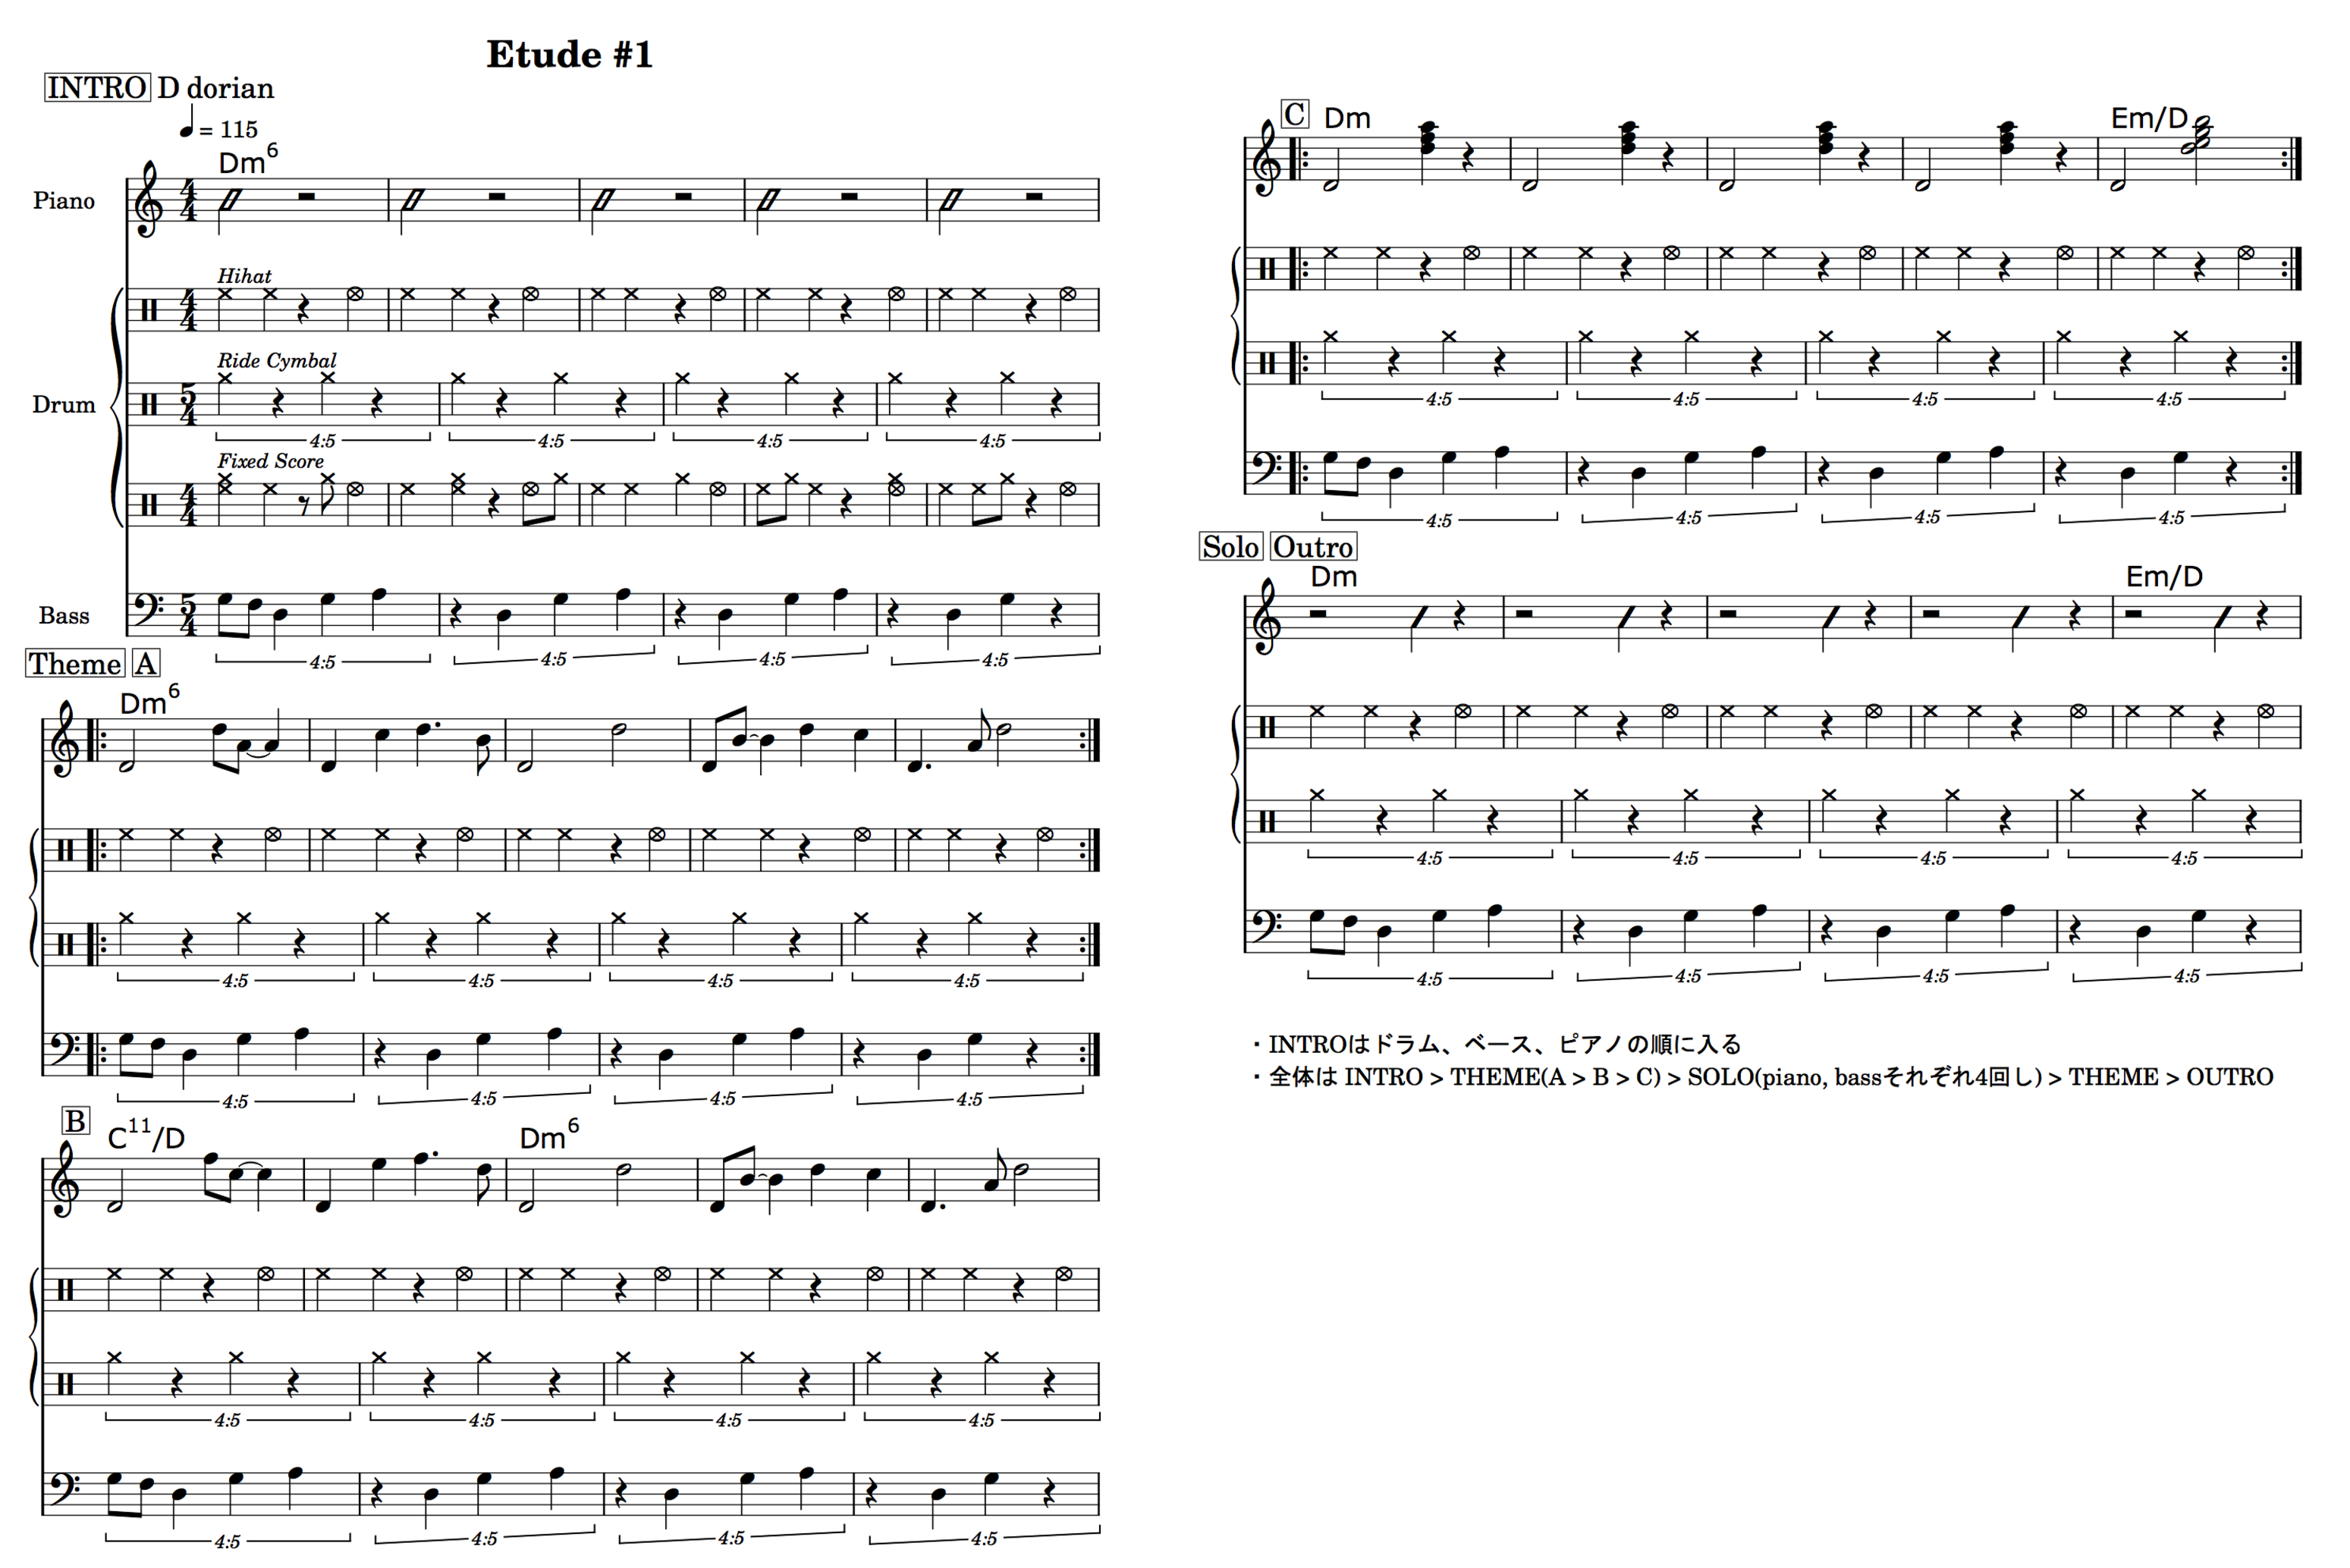
\includegraphics[
 width=\textwidth]{./PDF/figure_11.pdf}
}
\caption{"Etude \#1" lead sheet}
\label{fig:figure_11}
\end{figure}

"Etude \#2" features chord progressions compared to "Etude \#1," making the harmonic rhythm easier to feel, and the piece follows the commonly seen AABA form. However, in the B section, the melody and bass exchange their respective time signatures. Additionally, the explicit indication of rhythm by drums is reduced, requiring performers to generate the pulse of each time signature through mutual structural understanding, as shown in Figure \ref{fig:figure_07}. This piece has the objective of "acquiring application of music for multilayered temporal structures and rhythm exchange," and the composition was created with this intention. Figure \ref{fig:figure_12} shows the lead sheet for "Etude \#2."

\begin{figure}[htb]
\centerline{
	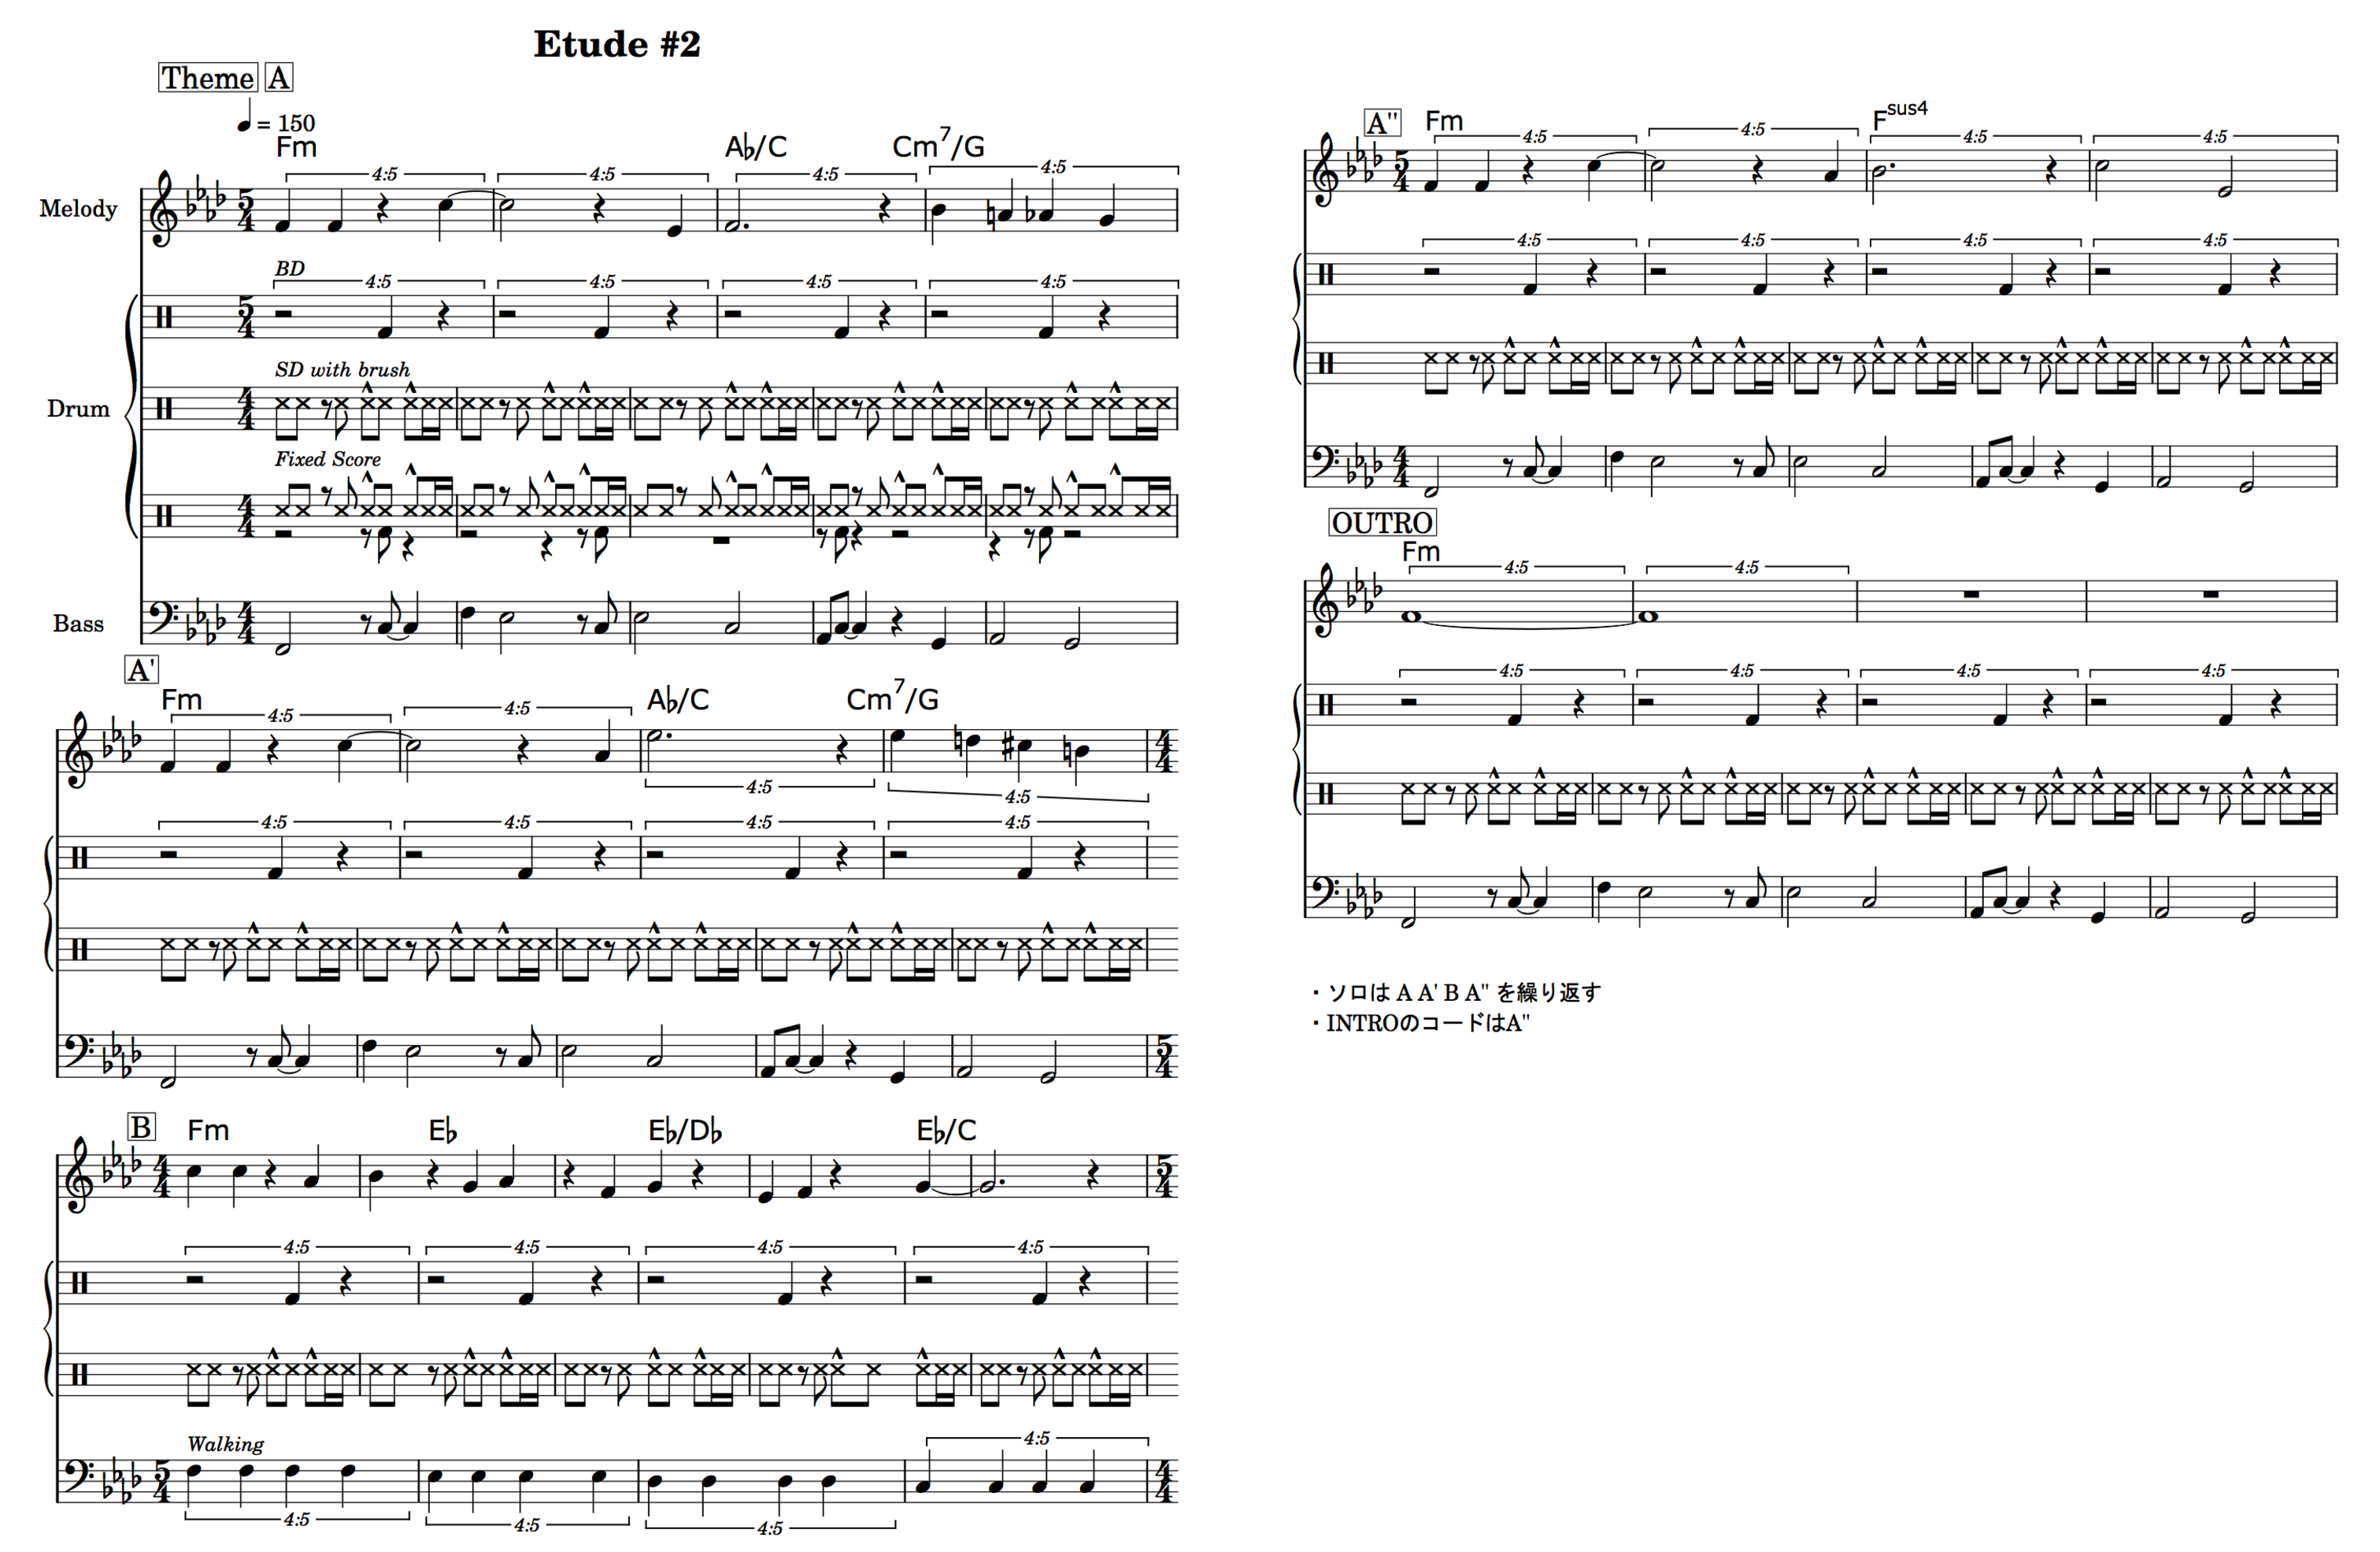
\includegraphics[
 width=\textwidth]{./PDF/figure_12.pdf}
}
\caption{"Etude \#2" lead sheet}
\label{fig:figure_12}
\end{figure}

"Etude \#3" distinguishes itself musically from "Etude \#1" and "Etude \#2" and increases difficulty by being composed in three layers: "3 beats in 4/4 time," "4 beats in 4/4 time," and "5 beats in 4/4 time." A significant feature is that this piece does not provide the drum assistance for each time signature seen in "Etude \#1" and "Etude \#2." Therefore, as shown in Figure \ref{fig:figure_07} for "Etude \#2," each performer must structurally understand their pulse from the piece and perform accordingly. Additionally, this piece features circular chord progressions, demonstrating "the potential for polytonality inherent in music for multilayered temporal structures." Figure \ref{fig:figure_13} shows the lead sheet for "Etude \#3." Each lead sheet can also be viewed in the work "Music for multilayered temporal structures" \cite{yamato:01}. The work can be downloaded from the following URL: \url{https://goo.gl/o1pTEk}

\begin{figure}[H]
\centerline{
	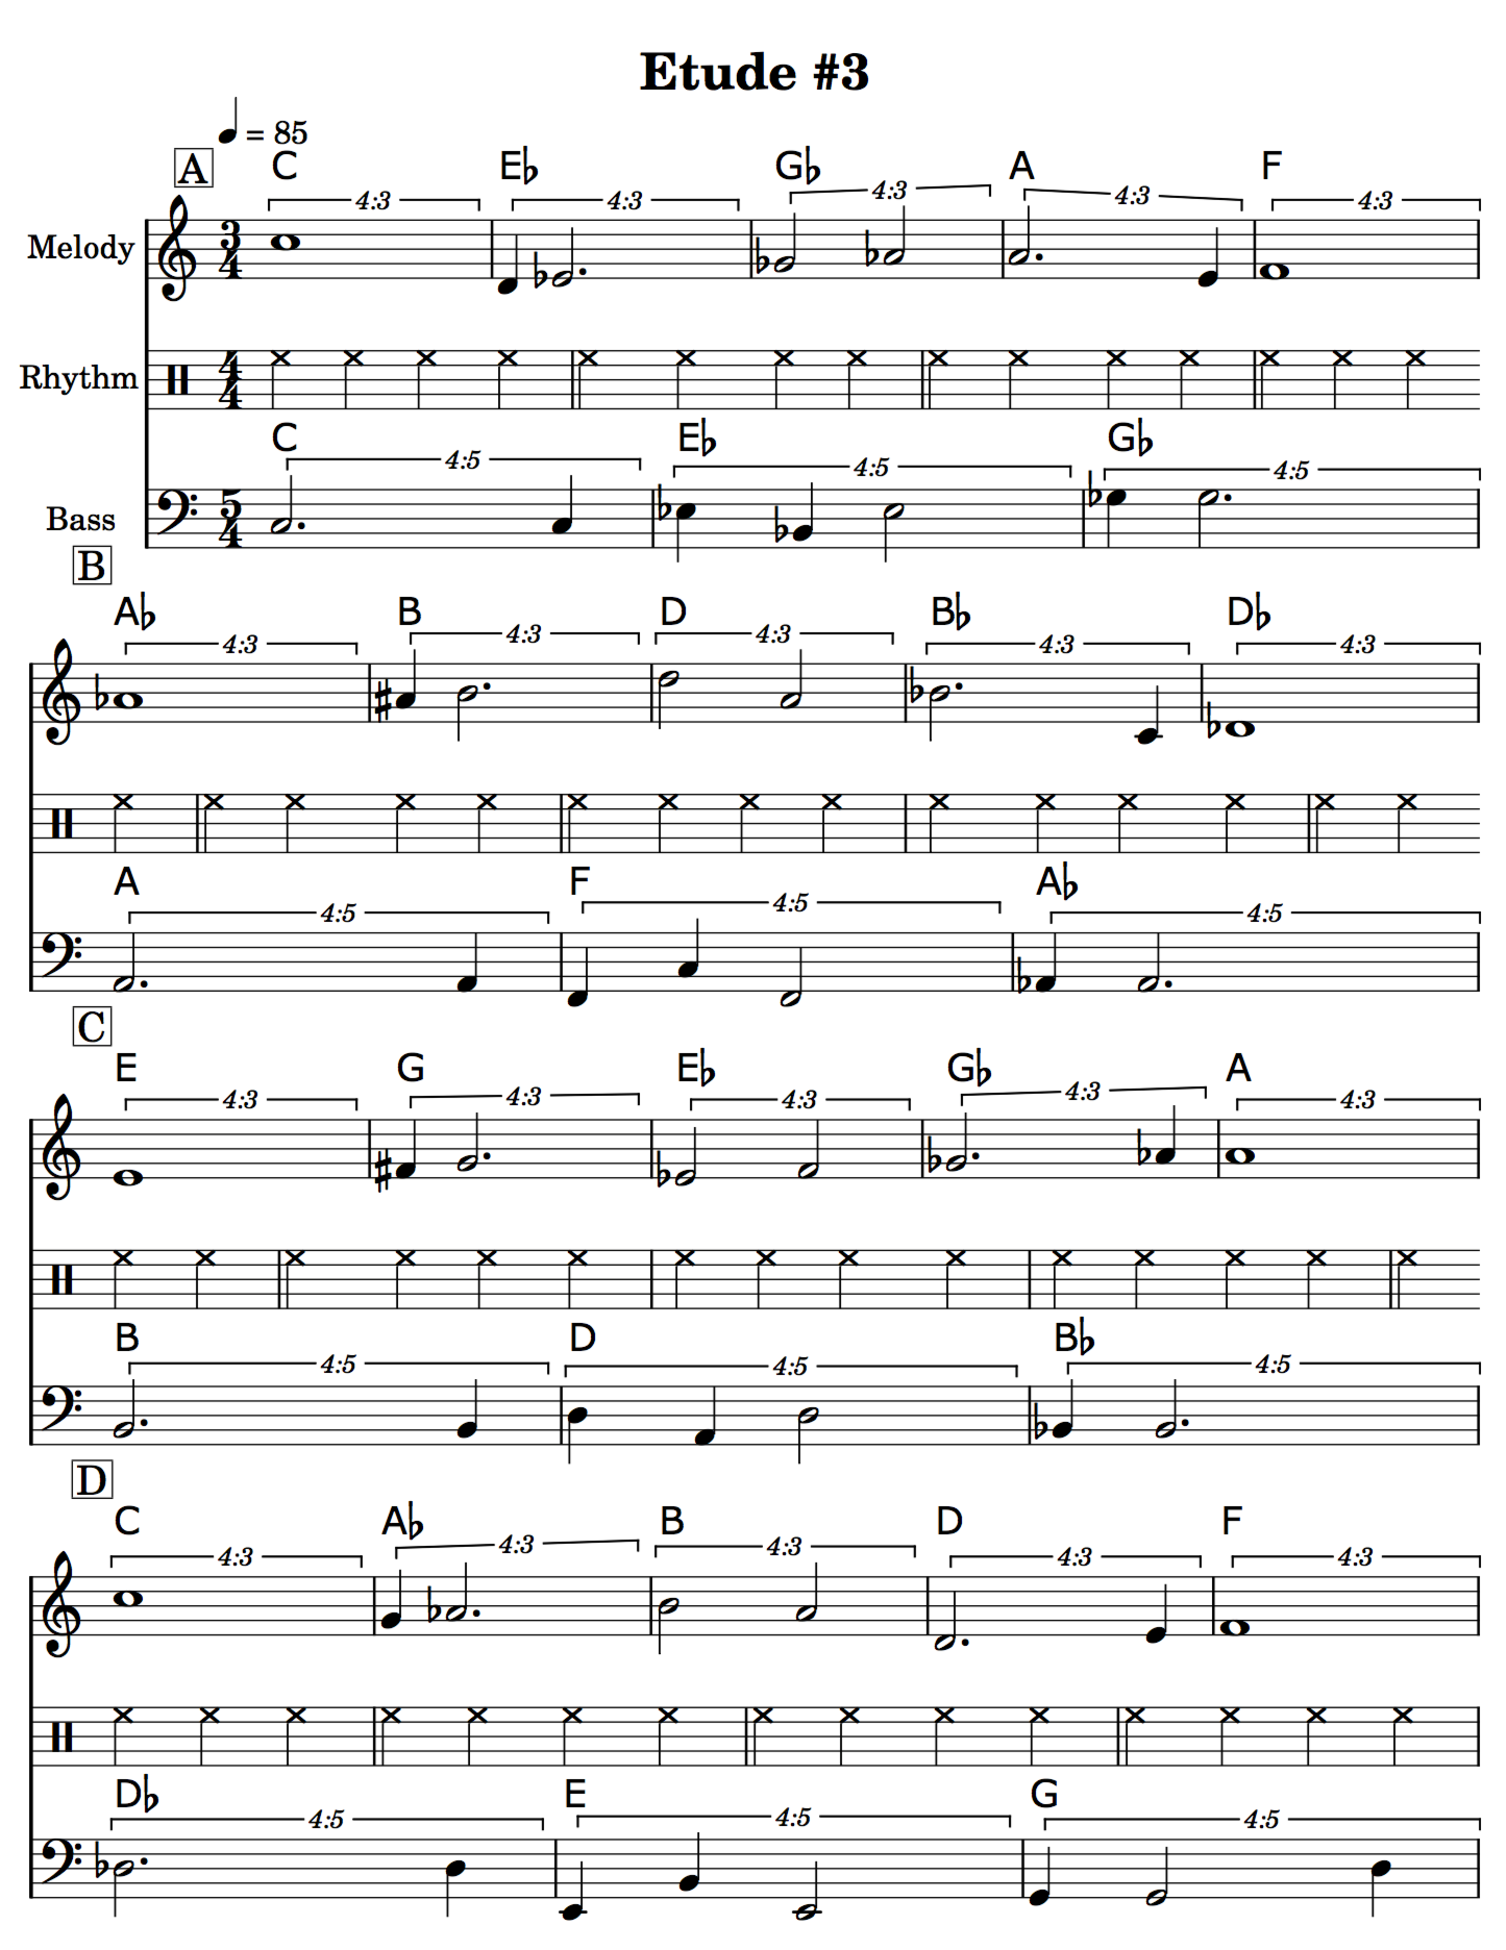
\includegraphics[
 width=0.5\textwidth]{./PDF/figure_13.pdf}
}
\caption{"Etude \#3" lead sheet}
\label{fig:figure_13}
\end{figure}

Summarizing the relationships between the above etudes, as shown in Figure \ref{fig:figure_10}, the difficulty gradually increases from 1 to 3.

\begin{figure}[H]
\centerline{
	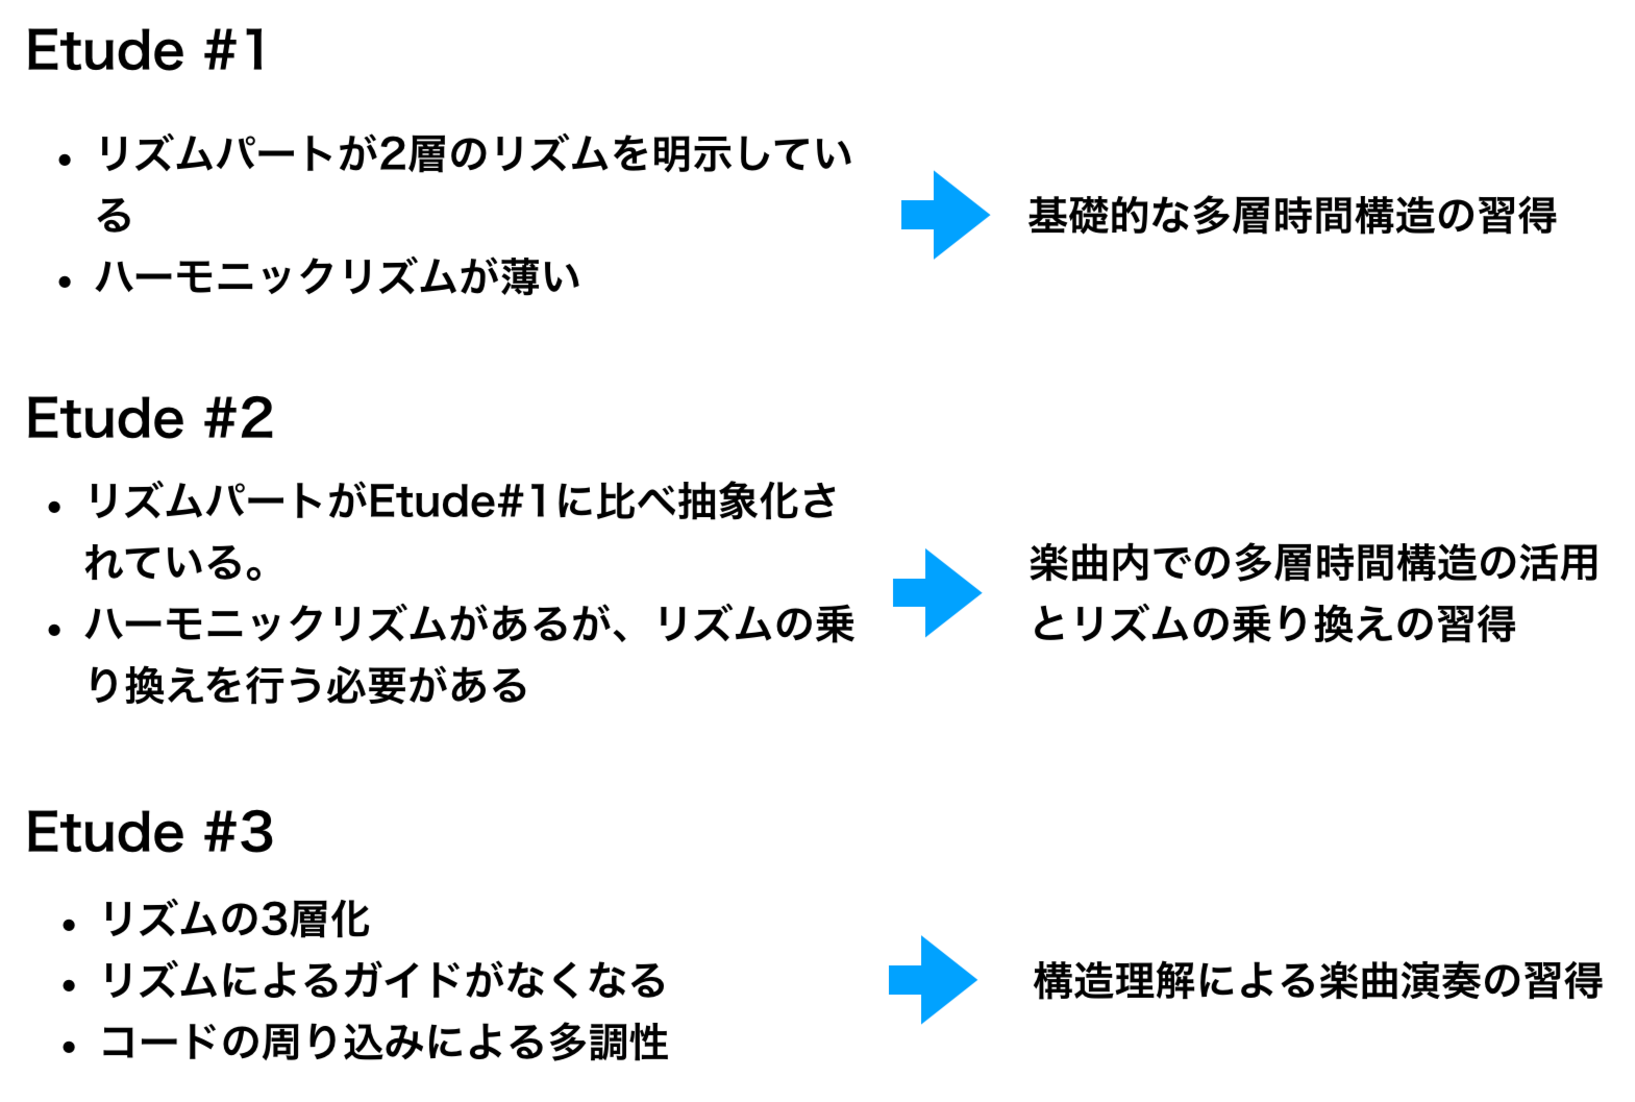
\includegraphics[
 width=\textwidth]{./PDF/figure_10.pdf}
}
\caption{Relationships between each etude}
\label{fig:figure_10}
\end{figure}

Each piece was created using Apple Logic Pro X, and simulation audio sources were produced. Each audio source can be heard at the following URLs:

\begin{enumerate}
	\item "Etude \#1" \url{https://goo.gl/Bv1odQ}
	\item "Etude \#2" \url{https://goo.gl/49g16U}
	\item "Etude \#3" \url{https://goo.gl/mzgDqu}
\end{enumerate}

\section{Possibility of Embodiment}

To verify the performance feasibility of the work ''Music for multilayered temporal structures'' described thus far, actual jazz musicians performed ''Etude \#1'' and ''Etude \#2'', which were recorded and documented on video.

The musicians who participated in the performance were three members in a so-called "piano trio" configuration: Tomohito Yoshijima on drums, Yuji Kawamoto on bass, and Masaaki Kaneko on piano. For this performance, the use of existing formats such as "lead sheets" and "piano trio" for the scores and instrumental arrangement was chosen because it was believed to connect to questioning "new music as popular music" rather than being merely a system or experimental approach for this "music with multilayered temporal structures."

The performance was conducted according to the following schedule:

\begin{enumerate}
  \item After determining the musicians, simulation audio tracks and materials were distributed
  \item The first rehearsal was held on 10/22 (Sunday) (drums and bass only)
	\item The second rehearsal was held on 10/29 (Sunday) with piano added
	\item At the second rehearsal, at the request of the bassist and pianist, the Apple Logic Pro X data of the simulation audio was also distributed
	\item Recording and filming were conducted on 11/10 (Friday)
\end{enumerate}

The recording and filming took place in a so-called "recording studio," where the performers were separated into different booths and played while listening to each other's performance through headphones. No click track was used during the recording. This video documentation is publicly available on the author's YouTube account as {\bf Video Documentation ''Music for multilayered temporal structures''}\cite{yamato:04}.

\subsection{Reflections on Rehearsals}

As indicated earlier, two rehearsals were held. The number and participants were determined by the performers' scheduling availability. In the first rehearsal, we worked with the drummer and bassist. Although audio and materials had been distributed in advance, the performers had not specifically practiced for the rehearsal by that day, so we first conducted a reading of the work (booklet) and explained the scores. At that time, the materials did not include explanations of "music with multilayered temporal structures" or "variable meter notation," so explanation by the author was necessary. However, regarding the rehearsal itself, after explaining that "in reality, the author does not exist at this rehearsal" in reference to the work concept, we emphasized the performers' autonomy and endeavored to observe as much as possible. The same approach was taken during the second rehearsal.

In the early stages of rehearsal, both the bassist and drummer tried to proceed with a "fixed meter notation" mindset, but it did not work well. They cited reasons such as "quintuplet quarter notes do not appear in the kind of music they usually play," "when thinking in quintuplet quarter notes, the tuplets cross bar lines when viewed from 4/4 time," and "the downbeat of the quintuplet quarter notes is a rest." Therefore, understanding was facilitated by explaining the structure of the piece as shown in Figure \ref{fig:figure_07} and demonstrating how to feel the rhythm. In this rehearsal, the bassist was unable to leave out the downbeat until the end and started by practicing playing all beats of the quintuplet quarter notes. The drummer proceeded with mastering first the binary division of 5 beats as a reference to understand multiple beats. When moving to ''Etude \#2'' in the latter half of the rehearsal, the transition was smooth, and we received comments from the performers about feeling the effectiveness of ''Etude \#1''.

Next, in the second rehearsal, the pianist joined for a rehearsal toward the actual recording. In this rehearsal, the pianist also initially took a "fixed meter notation" approach, but similarly found it difficult to play quintuplet quarter notes and felt ''Etude \#2'' was more difficult than ''Etude \#1''. Also, as before, after communicating that the author would remain as an observer as much as possible, the rehearsal proceeded, but when performers made structural changes to the music to reduce performance difficulty, this was pointed out and not permitted. For example, since ''Etude \#1'' is made in one mode of D Dorian, the position of rehearsal letter B in the piece was difficult to identify, so referencing {\bf ''So What''}\cite{miles:01}, a request was made to change it up a semitone, but this was not permitted. When actually tried once, while it made the overall structure of the piece easier to understand, we communicated that the purpose of ''Etude \#1'' was "structural understanding of multilayered temporal structures" and should be done in a minimal form. Also, on this day, there was almost no playing finer than quarter notes in the solo sections. This is believed to be because the pianist was trying to understand the quintuplet quarter notes in ''Etude \#2'' with fixed meter notation, converting one beat to five eighth notes in 4/4 time, and thus could not subdivide one beat of 5/4 time.

\subsection{Reflections on Recording and Video Documentation}

Through the two rehearsals, several issues were identified. As mentioned earlier, the bassist and pianist each practiced and approached the recording. ''Etude \#1'' proceeded relatively smoothly, but toward the end of takes, they became unable to complete the performance. Comments indicated this was because the load of each person keeping rhythm was higher than usual pieces. In ''Etude \#2'', it was observed that the pianist independently noticed that "the bass and drum attack points always indicate beats 1 and 3 of the piano." However, regarding the piano solo, the frequency of using notes finer than quarter notes was low, and when pointed out, there were comments that it was difficult to play. The bassist switched rhythms at the B section of ''Etude \#2'' by using the beat of the theme immediately before the B section as a trigger. Particularly in the solo, it can be seen that this part was well utilized.

Throughout the video, it can be observed from the body movements and head movements of the pianist and bassist that each is playing in a different time signature. Also, there were comments such as "during recording (while playing), I don't know what kind of music it is becoming," but on actual playback, "it sounds pop," and "it's like a notated {\bf ''Bitches Brew''}\cite{miles:02}, but I don't know of similar attempts to reproduce this with notation."

Regarding the recording, while there were some innovations and performance compositional ideas (such as the interlude-like development for returning from the solo to the theme in ''Etude \#1'', including the drummer's drum patterns), these did not involve changes to the overall structure of the score and remained at the level of on-site innovations by jazz musicians for performance, while still being able to reproduce the structure of the pieces. Through these rehearsals and recordings, the performance feasibility of "music with multilayered temporal structures" was demonstrated.

\section{Discussion}

\subsection{Analysis of Interviews with Performing Musicians}

Interviews with the performing musicians were conducted individually: with Mr. Yoshijima on December 15, 2017, with Mr. Kawamoto on December 18 of the same year, and with Mr. Kaneko on December 19 of the same year. The interviews were conducted as semi-structured interviews with predetermined topics aimed at investigating the musicians' subjective experiences regarding the following items, while prioritizing the natural flow of conversation and allowing free expression. The full interview content is provided in \ref{appendix}, so excerpts will be discussed here. The items are as follows:

\begin{enumerate}
  \item Impressions after listening to the video and audio recordings of this work
  \item Regarding the work's booklet, was the content understandable?
	\item Impressions of the booklet and whether there was any useful knowledge gained?
  \item Have you experienced any similar music in the past?
	\item Are there any differences compared to what you usually do?
	\item Where do you think the difficulty of performance lies?
  \item What do you think about the potential development of this work and method?
\end{enumerate}

\subsubsection{Regarding "Impressions after listening to the video and audio recordings of this work"}

Both Yoshijima and Kawamoto expressed concerns about whether actual performance was possible. This can be understood from Yoshijima's comment that "there is no precedent for such a score" and Kawamoto's remark that "there is content written in the score, but I wondered if this would be okay." However, both felt a gap between the score and the music, noting "it became music unexpectedly" and "it became more proper music than I thought." Kaneko also gave positive evaluation regarding the feasibility of performance. Concerning the score and actual performance, Yoshijima pointed out: "I don't know what kind of sound it will become when the three of us come together, or what kind of groove will emerge." Kawamoto also raised the point "I understood the concept, but I wondered if it wasn't impossible to perform," suggesting that he felt the difficulty from the work itself.

\subsubsection{Regarding "Was the content of the work's booklet understandable?"}

While Yoshijima and Kawamoto stated they "understood," Kaneko said "I haven't read it thoroughly enough, so it hasn't sunk in yet." As Kaneko mentioned in the interview that he was "approaching it as business," it appears he was viewing it from the standpoint of an ordinary "job" and focused only on what was necessary to complete the commission.

\subsubsection{Regarding "Impressions of the booklet and whether there was any useful knowledge gained?"}

Yoshijima, the drummer, expressed this attempt as "like having one rail, and although there should be another flowing in a different direction, somehow they're on the same rail," and stated that "I can already apply this within myself and bring it out in other situations," suggesting that understanding has progressed to the level of physical embodiment. On the other hand, Kawamoto noted "from a musician's musical information perspective, there are parts that are slightly over-explained. It could be simpler," while also stating "but the way the drum score is divided into two staves and such ingenuity is very good (omitted). It was very good for understanding the layers of music. The fact that it shows how this and this add up to become this was very good. As a score that appears in the field, it's unlike anything I've seen before, but I think it's sufficient as an explanation of the project," acknowledging a certain effectiveness of the booklet for performing this work.

\subsubsection{Regarding "Have you experienced any similar music in the past?"}

We were able to hear about many examples of polyrhythm/cross-rhythm in general and experiences of attempting them personally, but similarities to the characteristics of this work—such as the way rhythms are taken and the notation—remained at the level of "possible that similar things existed in the past." This is due to the impossibility of confirming all music, and comments were also heard regarding the possibility of analysis arising from the notation method.

\subsubsection{Regarding "Are there any differences compared to what you usually do?"}

Yoshijima's answer that "what I usually do is more difficult" is interesting. The reason being "when each person is only doing their own thing, even if I try to connect, it's impossible to hold them together," and compared to such situations, he wondered "is it easier when the performers are trying to connect?" When asked this, he responded: "That's really just a matter of whether it's musical. In that sense, for this piece, I felt more comfortable. No matter how high an individual's ability is, it's more painful in a field where people gather who perform selfishly." I speculate that this is also influenced by the fact that the drummer's role had a large proportion in connecting the parts. Additionally, Kawamoto expressed understanding of this research's positioning as "research on vocabulary," stating "I think it's research on grammar focused on one point, and it's something that really should be done, but normally it's difficult to focus that narrowly and spend time on just that one thing. That's why even though I understood the concept, I didn't know if I could perform it. That's why it's something very valuable," commenting on the research's value in comparison to his usual activities.

\subsubsection{Regarding "Where do you think the difficulty of performance lies?"}

Kaneko cited "because the rhythms are compound," pointing to the basic concept of this work. Regarding the difficulty, while stating "I've heard that when humans do two things, they can't do them at 50\% each but rather at about 30\%, making it inefficient. I think it's that kind of difficulty," he actually considered that "when humans process something like this time, I don't think they're doing it multitask. Isn't it similar to the drummer not processing multitask?" Yoshijima mentioned regarding solos: "when someone takes a solo, someone should be the foundation, but this time the drum had a large proportion of that, though the difficulty changes depending on who produces that pulse." As an example, he stated: "for instance, if the drums start taking a solo, to whom do we entrust the rhythm? I would probably destroy it with considerable force, so by doing that, I think the difficulty level increases further," suggesting that he considers the difficulty of performance to vary depending on relationships. I believe this is due to qualitative differences in performance arising from the width created by the piece being meta-composition and by performers' interpretations. Furthermore, Kawamoto pointed out regarding physicality, from the interpretation of "research on vocabulary" mentioned earlier, that "even if you learn a new word, to be able to use that word freely, you need to internalize it physically once," indicating that this takes time. However, regarding the amount of time, he showed that the proportion of usual experience is large: "I've never thought about 3 over 4 with the resolution used this time. In other words, I could play it because I normally listened, learned, and played repeatedly, so if I had normally only listened to and learned 5 over 4 songs, I probably could do it." This also connects with both Kaneko and Kawamoto expressing during rehearsal that the difficulty of "5 over 4" was due to not having opportunities to play it in regular performance.

\subsubsection{Regarding "What do you think about the potential development of this work and method?"}

Yoshijima cited that understanding of what he usually does in his activities progressed from the reproducibility that the score possesses. This means it is directly influencing Yoshijima's ongoing activities, suggesting the possibility that Yoshijima himself will develop/inherit it. Kawamoto cited examples of counterpoint and Bartók's quartets, suggesting that he recognizes its applicability more as a compositional method than improvisation.

\subsection{Analysis from Interviews with Musicians of Other Genres}

Interviews were also conducted with musicians of other genres who did not participate in the performance. The interview was conducted simultaneously with both Mr. Shinya Ando, a santoor player who is a performer of Indian classical music, and Mr. Jun Haraguchi, a tabla player. The interview items are basically the same content as the previous interview, except for some parts. The interview content is provided in \ref{appendix}, so excerpts will be discussed here.

% \begin{enumerate}
%   \item Impressions after listening to the video and audio recordings of this work
%   \item Regarding the work's booklet, was the content understandable?
% 	\item Impressions of the booklet and whether there was any useful knowledge gained?
%   \item Have you experienced any similar music in the past?
% 	\item Are there any differences compared to what you usually do?
% 	\item Where do you think the difficulty of performance lies?
%   \item What do you think about the potential development of this work and method?
% \end{enumerate}

\subsubsection{Regarding "Impressions after listening to the video and audio recordings of this work"}

Positive comments were observed regarding the characteristics of the work, such as rhythmic changes at the rhythm-switching parts of Etude \#2 and being able to take either beat. Additionally, Ando mentioned the difficulty as a solo performer, relating it to his own experience, and pointed out that to make it possible, "first everyone needs to be familiar with irregular time signatures, with an era when songs in 5 are normally abundant, and when that era comes, it will gradually become possible to enter suddenly with different rhythms." This indicates that in Ando's subjective view, the standard rhythm in the current music situation differs from this piece and Ando's usual experience.

\subsubsection{Regarding "Was the content of the work's booklet understandable?"}

While stating that understanding was possible by examining both the audio source and the score, Ando noted: "Since I've talked with the composer, I have that preconception, so I don't know if I could understand it if I saw this for the first time without knowing anything," reserving judgment about understanding the booklet at first sight. The author also understands that understanding the booklet requires a certain level of musical literacy, and considers this a valid point.

\subsubsection{Regarding "Impressions of the booklet and whether there was any useful knowledge gained?"}

Regarding the possibility of a performer playing two rhythms simultaneously through this research's attempt and what they are currently doing: "Since instruments like santoor and tabla can use both hands, there are various examples of two performers each playing different rhythms, but there have been no past approaches where one performer plays different beats with both hands, not in the way the drummer here is doing. Ando said in the summer, after meeting Yamato, that things he had been thinking about vaguely took form, and he's actually been doing that recently." This is similar to Yoshijima's understanding and application in the field mentioned earlier. I also speculate that being a percussionist may be related to applicability.

\subsubsection{Regarding "Have you experienced any similar music in the past?"}

Haraguchi cited an example performed by Zakir Hussain and Mickey Hart in 1976, "though it doesn't exactly correspond to this research's example." This is "an example of creating one melody within 102.5 beats according to the song's explanation," taking rhythm in a very large cycle. However, Ando stated: "What Zakir Hussain is doing is arranging and changing pieces, but the way of thinking is only Indian music. Even in Shakti and other things, he changes various things but only does Indian classical music," noting that the basic structure of the music is considered within the structure of Indian classical music.

\subsubsection{Regarding "Where do you think the difficulty of performance lies?"}

Ando stated that such attempts themselves are not difficult if you create something like the rhythm hit point tables shown in this paper, but cited "the time it takes to master." Additionally, noting that the difficulty differs between ensemble and individual, he explained: "When you try to do it alone. It becomes a bit easier to do it as a group, because once you learn how to fit it in, once it enters your own system, if you have in yourself how it goes in 5, how it goes in 7, how 3 goes, how 6 and 12 go, you can just fit them in there one by one, but for one person to start doing different things like this drummer takes time." This is interesting when considered in parallel to the relationship between Yoshijima and Kawamoto/Kaneko in this rehearsal. Yoshijima felt difficulty in showing the hit points of two rhythms alone to connect the bass and piano, and once he could do that, he became able to hear the entire piece. Kawamoto and Kaneko performed by learning what Ando calls "how to fit in," or in other words, the relationships. As Kawamoto mentioned in the interview, there was difficulty because it wasn't in their vocabulary, but as Ando points out, having such vocabulary within oneself makes it easier, which matches what Kawamoto himself mentioned as familiarity with 5 over 4.

Additionally, comments about how to listen to each other in ensemble are interesting. Regarding when Ando and Haraguchi perform polyrhythmic things, "When doing polyrhythmic tricks more than usual, the hit points must align so we're listening considerably. The side doing the original beat must not get pulled in, so while listening to the other, they do it like a metronome, but the side approaching is listening more, so to speak. They fit in phrases while listening," revealing differences in states of consciousness regarding hit points in polyrhythmic performance.

\subsubsection{Regarding "What do you think about the potential development of this work and method?"}

While Haraguchi relatively concretely mentioned his own performance, stating "there are elements of this that can be incorporated into my performance," both noted "if you analyze it carefully, you can't understand unless you really face it," but "if you listen to it as music, music that's really beautiful or something like that should spread more," which, regardless of whether this work is beautiful, matches the purpose of "at first glance you can listen normally, but structurally there's something complex behind it. Considering future music development in the context of popular music."

\subsection{Discussion on Composition and Production Environment}

This research, borrowing Kawamoto's words, focuses on rhythm within compositional methods as "research on vocabulary" in music. When viewing composition broadly through the works from there, as shown in \ref{Western-Modern-AmericanNewMusic}, if the compositional freedom before classical notation was established in the 14th and 15th centuries had remained in the present day, such music might have been possible. Additionally, the possibility that similar examples might exist in existing music due to what becomes invisible/visible through notation methods can also be said from the interviews. When considering composition from there, if current compositional methods, whether Western music or popular music, are established by the structural way of thinking about notation that is currently common, then just as Western music could not fully grasp African rhythms, it can be said that possibilities still remain for rhythm as a compositional method.

Furthermore, when considering the act of composition from the act of notation, if scores before lead sheets are analogized to the relationship between "computer programs and compilers," lead sheets can also be understood like the relationship between "structured data and AI." This can also be considered as a difference in physicality, apart from the body in Western music that "reproduces or expresses according to the note values and temperament of the score," as "a body that reproduces structure" in popular music.

Of course, it is self-evident that various musicians are currently taking all kinds of approaches not only to rhythm, so neither is this approach uniquely novel nor are existing approaches becoming obsolete. However, I consider that through the act of composition in popular music in this paper, while considering possibilities for future music to come, it becomes a critical attempt regarding the current state.

If this research is "research on a certain vocabulary," then beyond this research it is possible to develop and inherit toward other vocabularies, or vocabularies that can be considered in relation to this vocabulary. This is evidenced by various styles of popular music that continue to be inherited and developed even today through not only music theories such as from the Schillinger House to the Berklee Method and the Lydian Chromatic Approach in popular music history, but also through bebop, modal, free jazz, noise, and other genres.

In the works created as "music with multilayered temporal structures" this time, we could observe inadequate production environments during the production process. For example, as far as the author investigated, only with Lilypond was it possible to "structurally" describe scores with variable time signature notation. This is also one manifestation that notation presupposes the musical structure currently taken for granted. Additionally, regarding music production software, we could not find software that allows multi-BPM or track settings with multilayered time signatures, and in creating demo recordings, we could only produce in a method that "forced consistency" halfway using Logic Pro X's MIDI stretch function. Of course, it might be possible by making full use of MIDI resolution and placing MIDI data through calculations. However, that can hardly be called a "compositional method from the composer's subjective perspective" as shown with variable time signature notation. I consider that this research has also become a critical attempt regarding existing production environments in that sense.

\section{Conclusion}

As stated in \ref{research_target}, this research aims at the future development of "popular music" and focuses on rhythm. The method of "music with multi-layered temporal structures" conceived in this study can be summarized as follows based on the current results. First, "performance is possible through structural understanding without possessing exceptional technical skills." Second, "this approach can create music that lies within the extension of popular music context while being difficult ensemble pieces." Finally, "production and understanding require the development of notation and production environments." The performers in this study have professional careers, but they do not regularly engage in activities specializing in playing such music. However, in this case, they were able to perform based on their own understanding through lead sheets as meta-structures and their instruction manuals, as well as facilitation that promoted structural understanding. Furthermore, the author succeeded in composing pieces with conventional forms like "Etude \#2" and pieces within the jazz context like "Etude \#1" using the method of "music with multi-layered temporal structures" described in this paper.

The author already had experience learning the Berklee method when creating these pieces, which contributed to the success of the aforementioned compositions. One reason why the Berklee method developed popular music is that "Berklee College of Music did not impose restrictions when spreading its theory." In other words, the theory spread worldwide as musicians who studied at Berklee became educators themselves. Similarly, research on such methods holds great significance when it is made "open access" and "inherited or developed." In this sense, as understood from the interviews in this research, although limited in scope, this study has led other musicians to attempt to update their own musical expression. The author believes this is a greater achievement than the novelty of the research itself, when viewed from the perspective of "thinking about future music from popular music," which is the purpose of this research.\\

Finally, I will discuss future prospects from this research.\\

First, in order to explore the possibilities of rhythm through pieces with such structures, I would like to develop rhythmic cognition and structural understanding of music obtained from this through the development of production environments. This could include harmonic development, co-creation with computers using algorithms and AI, and the possibility of "welcoming such environments as performers or collaborators." Additionally, I would like to continue performance activities with the performers from this study and continue considerations on rhythmic cognition through interviews and collaborations with performers from other genres.

Regarding the development of the concept of "multi-layered temporal structures" proposed in this research, I consider the following. First, expansion into new harmony that could be created from the methods proposed in this research. By considering harmonic development together with multi-layered rhythms using the simple techniques shown in this research, there is potential to create new methods of harmonic development as an alternative to conventional harmonic extensions. As one attempt to demonstrate this possibility, "Etude \#3" was composed by dividing the same chord progression rules into two time signatures. With such a method, triads with simple sonorities can wrap around, and the harmonic sound necessarily becomes more complex/polytonal/atonal as time progresses. In improvisation, performers sometimes "assume" harmony different from the chord progression written in the lead sheet and perform with their own extensions/interpretations, but by conducting such harmonic extension concepts in relation to rhythm, the unique harmonic design that "multi-layered temporal structures" possess could be possible from the composition stage, and if used as an improvisation method, it could be effective as an alternative approach to conventional methods. Also, as a possibility for embodiment, by taking up the relationship with physical expression such as dance, it is necessary to consider not just the viewing experience, as with performance, but the process of how dancers themselves "embody" polyrhythm/cross-rhythm. Through such attempts, there is potential to create relationships not as a master-servant relationship like "dance and its background music," but as a relationship as "performers who create the music listening experience" together, and similarly in relation to other timeline arts such as video works, to create "new listening experiences in bodily sensation." There is still ample room for the development of musical art derived from rhythm.

\section{Appendix \label{appendix}}
\subsection{Interview with Participating Musician 1 (Tomohito Yoshijima, December 15, 2017)}

\begin{description}
 \item[Impressions after watching the video and listening to the audio of this work]\mbox{}\\

 There is no precedent for music with such scores. It was difficult to create, so I didn't know what it would be like until it was finished. When it became a video, it surprisingly turned into music. Then I felt like I could get more ideas from watching the video.\\

 --- {\bf What was impressive during the recording was that you said, ``I don't understand what's happening while I'm playing.''}\\

 The understanding from the first playback to the second playback was fast (because I was listening to the playback). We were able to discuss in the booth about ``let's do it this way.'' Once it was completed and the form was decided, there was a feeling that we could control something, like a photo of a completed plastic model, or ``we're going to make this now'' - that kind of understanding emerged. The score was like an instruction manual, or rather, in recording, the playback of what we performed became like an instruction manual.\\

 --- {\bf Was it at the level of not understanding the content of the booklet, or was it the category of understanding the booklet as a booklet but not knowing until you tried it?}\\

 I could simply read the score. But I didn't know how it would sound when three people came together, or what kind of groove it would become. I think groove is the most difficult thing now, because you can't write groove in a score, like fluctuations. That's where my attention goes.\\

--- {\bf Also, drummers are generally not thought of as harmonic or melodic instruments in the world, but on SNS, Yoshijima-san occasionally expresses concern to composers about what the groove is like, and how to react to the surrounding sounds. You want them to care not just about ``what's happening?'' and improvisation, but also about rhythm, while you yourself show interest in harmony and improvisation lines. Is this attitude of holding interest something that all drummers have, or is it unique to you, Yoshijima-san?}

I simply think there are two patterns: people who originally played piano or guitar may be concerned about what's happening now with melody or harmony, or their ears automatically go there. People who started with percussion instruments, especially skin instruments, don't go there and listen at a completely different place.

\item [About the work's booklet, could you understand the content?]\mbox{}\\

There was nothing I couldn't understand. I could read it normally.\\

--- {\bf There were parts that weren't written in the usual notation, but you could still read it without any problems?}\\

It's just that you can read each part separately (so I could read it). The difficulty is when it flows simultaneously, but I can understand each individual thing that's written.\\

\item [About the booklet, were there any impressions or useful insights for you?]\mbox{}\\

For example, if there's one rail, and there's supposed to be another flowing in a different direction, but somehow they're on the same rail - that kind of sensation only comes out if you do music like that, and it became audible to me while performing. So I've already been able to apply it within myself, and I can bring it out in other situations, which is the cause of recent incidents.\\

--- {\bf It's amazing that you're using it in the field.}\\

When I started using it, nobody understands, after all. But depending on the person, they challenge on their side, so some bravely say ``keep it as it is.'' It's in a state where (beat) counting is not allowed, or rather, you can't count from the second beat onwards. Since I'm used to it, I can perform without a running start. I've gotten used to the state of dividing into 4 while deviating from the four beats that I was counting ``one, two, three, four'' until just before, so I can change it within myself. When asked to ``do an open solo,'' I do it ``intending to make them regret it.''\\

--- {\bf In an open solo, you can't tell where the downbeat is, right?}\\

I've also gone to that side, so I can't go back. You can't discard what you've learned, right? Once you get used to it, you want to try it in the field too.\\

\item [Have you experienced any similar music before?]\mbox{}\\

Similar examples to this are difficult. As I pointed out during the recording, if you write Bitches Brew in a score and try to create that unique atmosphere, you might need a score like this. But I've never seen the opposite pattern like this time. I hadn't yet had the experience of it being written in a score, and as a result of performing it, it became like Bitches Brew. However, by doing this kind of score this time, there might be something close to this in what Mr. Kikuchi was doing, or what Tipographica was doing.\\

--- {\bf I think knowing or not knowing that notation changes the analyzability of the music you listen to. If you write the notation like that, you might think ``maybe this music can be analyzed,'' but in the case of polyrhythm/cross-rhythm, sharing the bar line is a prerequisite, and in the case of wrap-around, sharing the beat is a prerequisite - it seems like there's only one or the other, and this time you're doing both.}\\

For me, there's surprisingly neither, and I read and perform melody first, so I only think about where to breathe. For instance, if there's music in 5 beats, even if the music's rhythm is in 5/4, if the breathing place is ``one, two, three, four, five, six'' at the end, I perceive that as one unit. So actually I might not be counting time signatures. Everything is in 1 beat.\\

--- {\bf That's like Indian musicians (in the sense of accumulating).}

So, I've performed Frank Zappa's Black Page before, but I don't understand what's difficult about it. You just have to read everything. The hi-hat is playing quarter notes. I understand (technically) that the difficult part is the many tuplets, but since you just have to read it, I've never thought it was difficult.\\

--- {\bf Music like Black Page is a virtuosic piece of contemporary music style. Compared to that difficulty, if you just look at the lead sheet of the piece you performed this time, anyone could perform it. But in reality, everyone said it was difficult, difficult when performing. What do you think is the difference in difficulty?}\\

It's that this time, it's not that each individual line is difficult, but the ensemble is difficult. For example, if three people have to do it, you hear completely different things, and within that, you have to maintain the pulse you need to put out. On top of that, if we compare with Black Page, Black Page has the quarter note decided. The performers ride on top of that to perform, so the difficulty of Black Page is that it's difficult for everyone to unison such odd tuplets together. So if you do it alone, it's not difficult.\\

--- {\bf If you feel like singing, you can sing Black Page by yourself.}\\

Because you just have to read what's written. But this time's piece, even if you read what's written, one line alone is meaningless. So it's an etude for ensemble practice, not for individual practice. However, what a drummer does to make it work as an ensemble is to hold the other parts together. So in the middle, how to make those misaligned beats into one within your body - this kind of solo ensemble is the first time.\\

--- {\bf The talk of holding together came up, but from an outside perspective, I thought Yoshijima-san was the one who understood best what the music was doing among the three. The other two were saying things like they didn't quite understand ``what's correct,'' but only Yoshijima-san could say ``that was correct now'' - a situation arose, and I think there's a difference in the role of the parts.}

\item [Is there any difference compared to what you usually do?]\mbox{}\\

Conversely, situations where I'm required to play normally are more difficult. When each person is only doing their own thing, even if I try to connect, it's impossible to hold it together.\\

--- {\bf Is it easier this time when everyone is trying to connect?}\\

Yes. That's ultimately only about whether it's musical or not. In that sense, this piece was more comfortable for me emotionally. No matter how high the individual abilities are, situations where people who play selfishly gather are more painful.\\

--- {\bf This time, watching the recording, the performance didn't rush (the tempo didn't gradually increase), but I thought maybe this music doesn't allow such things. Because everyone is trying to maintain the structure. Of course, there are higher levels, so I can't say that definitively based on this time alone, but what do you think?}\\

As we get used to the piece, we naturally want to challenge. I think rushing or dragging happens with that challenge image.\\

\item [Where do you think the difficulty of live performance lies?]\mbox{}\\

I think the most difficult thing is that you have to ``solo'' after grasping that. I think it would be good if someone could be the foundation when someone takes a solo, but this time the drums had a large proportion of that, but the difficulty changes depending on who puts out that pulse. For example, if the drums start soloing, who do you entrust the rhythm to? I would probably destroy it with considerable momentum, and by doing so, I think the difficulty increases further.\\

\item [How do you think about the development potential of this work and method?]\mbox{}\\

It's difficult, maybe it already existed. This time it's a special case of creating it from a score, but surprisingly when you listen to it, there was this ``this sounds like this,'' so maybe there won't be visible changes, but the fact that it can be controlled with a score is frightening. For example, things that were randomly entered in electronica like ``it's randomly entered but feels good'' - now it's controlled. I think there's tremendous progress in terms of reproducibility. The strength that this can be heard again. And it's not left to computers but performed by humans. This is frightening.

--- {\bf Is the point of the current discussion about reproducibility through scores?}\\

People like me who are eccentric are pleased. When playing randomly, you say ``I wasn't in good condition today,'' right? Like, we didn't match well. That disappears - I feel like stress is removed. Because it's visible that if you do this, you can produce the sound you want to produce - even if it's a minority, it really helps me. I don't have to fight anymore.\\

--- {\bf It's amazing that Yoshijima-san is developing or inheriting this rhythm in the field and using it. Is there anything about this entire project that hasn't come up yet?}\\

The performances I've done until now, even in my mind, are not very clear, and I wonder where my ambidexterity comes from and where it lands - this was one answer to that. But no one could systematize it, and even in my own head, it wasn't something that could become systematic. But what's interesting is that even though I was doing it before, when I was given the score and tried to do it, I couldn't. I got it to fit perfectly just before the recording, and I thought ``this isn't much different from the performance I always do.''\\

--- {\bf I think this work, rather than strongly asserting novelty, merely shows one way that occurs simultaneously and spontaneously as popular music?}\\

What's happening now is the same as what Berklee did with what Charlie Parker was performing, and I think Parker might think that if his performance hadn't been analyzed, jazz wouldn't have developed so much.\\

--- {\bf Historically, jazz is highly analyzable music, and it spread widely because Berklee Method fit into it, right?}\\

That's right. Whether that analysis is correct or not, various ways of thinking came out based on that, didn't they? In some cases, as if to deny that, Miles started doing modal. But then it was chaos, and nothing more came out, so there's a background of going to free jazz, but actually it came out, like this. The fact that it has reproducibility is enormously significant. But whether anyone can do it is a different story, including whether they want to do it.
\end{description}

\subsection{Interview with Participating Musician 2 (Yuji Kawamoto, December 18, 2017)}

\begin{description}
\item[Impressions after watching the video and listening to the audio of this work]\mbox{}\\

The impression was that it had become proper music more than I thought. That's due to playability issues and also the content written in the score, and I thought ``will this be okay?'' but it became more comfortable to listen to than I expected, so that was good, and at the same time it was mysterious or interesting.

--- {\bf In what way was it interesting?}\\

Such rhythm figures are written with music theory matters as the main focus rather than musical matters first, right? Because it's research with a purpose, that's fine, but when we actually performed and recorded it, it became a good balance, and I don't know if that's just because our ears got used to it, or the work was originally good, or the performers' ability - I don't know which, but I'm very satisfied with what was completed.\\

--- {\bf Behind the words ``it was more musically viable than I thought,'' I think there's the thought that ``it might not work,'' so what kind of non-viable state were you thinking of?}\\

I was thinking that. I wondered if it would be okay. I understood the concept, but I thought it might be impossible to perform. That was the biggest thing. Next, because there are many research constraints, the arrangement of notes written there might not sound like melody, and if it doesn't sound like melody, it won't become music. But it sounds. Especially Etude \#1 - I thought ``will this be okay?'' but I think the performers' ability was significant.\\

--- {\bf What do you think about the criticism that might be received that ``the performers are just matching it''?}\\

This is the dilemma of such research - when the criticism ``aren't the performers just matching it?'' comes out, from a musical perspective, ``what's wrong with matching?'' Even if there's a physical problem of whether such an attempt is possible or impossible as a research theme, as a performer's final responsibility, we have to make something happen, so ``we couldn't do it'' or our pride of course, and the desire to contribute to research is also there, so from that standpoint difference, the sense of the musical field is ``what's wrong with matching?'' I think that contradictory position always emerges in doing such things. I think it's about how to twist that down as a work.\\

\item [About the work's booklet, could you understand the content?]\mbox{}\\

Of course I could understand. There's more than enough explanation.\\

\item [About the booklet, were there any impressions or useful insights for you?]\mbox{}\\

This won't directly answer the question, but from musicians' musical information perspective, I think there are parts that are slightly over-explained. It could be simpler. However, I thought the innovation of dividing the drum score into two staves was very good. I made my own programmed sound source for practicing at home, and such things were very good for understanding musical layers. It was very good that it showed that this plus this becomes this. As a score to come out in the field, it was something I'd never seen before, but I think it's sufficient as a project instruction manual. Also, the talk about cognitive dissonance was interesting. Very Yamato-like.\\

\item [Have you experienced any similar music before?]\mbox{}\\

I think there are many similar examples, and jazz in general is like that.\\

--- {\bf Generally, when poly is happening, the bar lines are shared, and phrase wrap-around has shared beats. If the characteristic of this work is that neither bar lines nor beats are shared, and what's shared is the pulse at the least common multiple with large blocks, then are there similar examples?}

That's difficult. There might be in classical works, but I can't say this specifically, but in jazz, such things can probably happen during improvisation, and I think Evans was probably doing it, and Tony Williams in Miles' band was probably doing it.\\

--- {\bf This time we used variable meter notation, but usually we don't analyze like that. Because the analysis method is done in the form of Western music or Berklee notation, we didn't understand, but if you analyze Tony Williams etc. in variable meter notation, you can imagine you'd find he was doing similar things.}

That's probably true. As Yamato-san says, not limiting to Berklee, using staff notation and bar lines itself is a Western system, a Western European folk music system, and for example, Indian music uses different notation, so when you look at it with such different vocabulary, it's not strange at all that there are different analysis methods or analysis methods most suitable for music with such structure.\\

--- {\bf When African poly is transcribed in Western musical notation, Western music misses African poly - this is written in Kenichi Tsukada's ``The Truth about African Music,'' and they're missing it because they don't have the perspective of what kind of bitmap or structure to view it as.}\\

In that case, from the perspective of doing jazz, the rhythm of ``swing'' is impossible to notate on staff notation, so I don't trust scores very much to begin with. Also, there are five types of beats in jazz, and great performers like Parker firmly control which position they're performing at for one pulse. Laid back is also laid back, but there are two types of laid back, and they control that. Why jazz became like that is because I think the African people's ethnic subtle off-score concept was inherited directly into jazz, and surprisingly, that's passed down orally, not in scores - that's the fact. I think that's something unique to Black people when considering jazz's ethnicity. Japanese people aren't that interested in continuous rhythm.\\

--- {\bf Don't you think there's something common with Robert Glasper's rhythm sense?}

I think that also came out from past context, and jazz musicians have high affinity because the roots are the same, so I think it came out from such context. I read Gunther Schuller's book ``Early Jazz,'' and Gunther Schuller writes that the subtle deviation of fine pulses in African ethnic rhythms is not accidental deviation, but jazz giants like Charlie Parker and Dizzy Gillespie were doing it while recognizing it.\\

\item [Is there any difference compared to what you usually do?]\mbox{}\\

I think this time can be said to be ``vocabulary research.'' Vocabulary is very important whether composing or playing, but beyond that is ``what do you want to say?'' - when making music, we do all of that comprehensively, but I think it's grammar research with focus on one point within that, and I think it's something that really should be done, but usually we can't spend time focusing on that one thing to that extent. That's why I understood the concept but didn't know if I could perform it. That's why I thought it was very valuable.\\

\item [Where do you think the difficulty of live performance lies?]\mbox{}\\

Even if you learn new words, to be able to use those words freely, you need to physically internalize them once. Isn't that where it is? In other words, ``it takes time.''\\

--- {\bf When physically internalizing, you seemed to struggle with 5 beats in 4/4?}\\

Because I don't usually experience it. What I understood this time is that I normally do 3 beats in 4 or 2 beats in 3, but why I can do it is because I usually do it. I've never thought about 3 beats in 4 with this kind of resolution this time. In other words, I could play it because I repeatedly listened normally, memorized, and played, so if I usually listened to and memorized songs in 5 beats in 4, I could probably do it.

--- {\bf In that sense, were the simulated demo sound sources useful?}\\

Of course. In the sense of physically installing, I can't say it was useful because I made practice karaoke myself, but for the demo sound source, the bigger issue is whether it sounds like music, so the surprise of ``so it becomes like this'' was bigger. After that, it was a feeling of processing it in the field.\\

\item [How do you think about the development potential of this work and method?]\mbox{}\\

When I saw this work, the first thing I thought of was Bartók's string quartet. This becomes more interesting if you apply it to counterpoint. Rather, I think Bartók and Stravinsky are doing it. But isn't it applicable anywhere? I thought I'd do such things in my own songs. So in that sense, I thought about analyzing it. If you only follow the vertical lines, you don't really understand what's happening, but when 5 phrases or 4 phrases coexist, the chords that happen incidentally become the music's coloring - you can make music with that way of thinking, right? If you decide on tonality or decide on scale. Then I thought it would be useful for counterpoint-like things, and it's good to do it during improvisation, and that's like what Yoshijima-san is doing in the field, but if you suddenly do it, everyone would be surprised.\\

--- {\bf It's similar to Miles' reference to Tony Williams.}\\

Even if it's a word thought out logically, if it doesn't convey to people, it's meaningless - or rather, if you suddenly start speaking words that don't make sense, there's the aspect that people around don't understand, so I think that's really difficult, but still, such things should be done, and not in improvisation but properly done within musical pieces.\\

--- {\bf Firmly holding it as structure?}\\

Yes.\\

--- {\bf If asked about this research, it's not about novelty or anything, but I think ``the value is in describing such structures, making them viable as music, and performing them live''?}\\

I think this is like Matsuo Bashō. In other words, it's ``research on new vocabulary.'' It's ``research on new expression methods.'' It's not a matter of novelty or such problems, it may be new, but.\\

--- {\bf Popular music occurs contemporaneously, so asserting novelty doesn't make much sense.}

Going as far as a new format might be too much, but for example, if you divide 5 beats into 4, you can express fuzzy fluctuations that couldn't be expressed with sixteenth notes before, right? Based on that, there's the possibility of creating music with different expressions that's more seamless. Research on that vocabulary - it's like not just blue or red but purple, or yellow mixed into purple - such expressive range expands, right? If you can properly hold that in your physical being and use it freely, that's an enormously big thing. So it's like Matsuo Bashō - fitting your words and sensations into 5-7-5, though Bashō's vector is opposite, if you research like that, Bashō doesn't need to speak sentences. Such expression became possible. So it's the same - if you do more refined research, the expressive range will expand more. I think everyone thinks so, but when active jazz musicians do it, it comes down to how much value they find in terms of time. When you remove the cost-performance issue, there's nothing more interesting than this.
\end{description}

\subsection{Interview with Participating Musician 3 (Masaaki Kaneko, December 19, 2017)}

\begin{description}
\item[Impressions after watching the video and listening to the audio of this work]\mbox{}\\

Nothing in particular, but normally like ``we did it,'' ``we made it this far,'' ``amazing.'' The feeling of ``amazing'' from the side that performed. I often create from zero to one, so I understand very painfully how hard it is to do this far. In that respect, rather than how the research is, I think it's wonderful that ``such a result was produced.'' Moreover, considering the detailed scheduling and path to get there, it's heavy. You can think anything or express anything, but getting there is tremendously difficult. As for the evaluation of live performance as a research experiment, it's not for me to say, but with theory-oriented experiments like this, it's almost impossible to tell if it's useful or not, and there are many such parts, so there's no way to evaluate. Conversely, not at that level, but I'm evaluating that it was made, and there are almost no such people. Jazz musicians too make their own CDs, and when they think something, they can take action, but they don't actually do it. The fact that it was actually done is amazing.\\

\item [About the work's booklet, could you understand the content?]\mbox{}\\

If I read it with great determination, what they want to do would probably be conveyed, but just reading it superficially doesn't convey it. Since I haven't read it carefully, it hasn't entered me yet. I can't judge yet what it would be like when I read it carefully.\\

\item [About the booklet, were there any impressions or useful insights for you?]\mbox{}\\

Regarding rhythm, there certainly is much to think about, and human rhythm cognition was a point of interest.\\

\item [Have you experienced any similar music before?]\mbox{}\\

There are simpler ones. But not with 5 beats and 4 beats. I haven't crossed but made it poly, but in my own musical experience, I've practiced and used in improvisation things like dividing into several, but it doesn't go to poly. There's 3 or 4, but I've never done it that far. But there's nothing like mixing poly and cross.\\

\item [Is there any difference compared to what you usually do?]\mbox{}\\

I don't fully understand what the purpose of cross and poly this time is, but what I usually do is, to put it flatly, a business approach, and that's the difference.\\

--- {\bf In that sense, this relationship is also a business relationship of requesting and completing performance of a business piece. On top of that, I thought I could see the pride as a performer of ``if we can get this far, it's complete''?}\\

That's also there. It's a part I'm personally imposing on myself, probably a part I can't personally forgive. But if the director or producer says ``OK,'' there was also that aspect of having to stop there. That inevitably exists. But when involved, I think there's such a growth instinct.\\

\item [Where do you think the difficulty of live performance lies?]\mbox{}\\

It's because the rhythm is compound, right? Simply that. To put it simply, I thought multitasking is difficult. I've heard that when humans do two things, they can't do 50% each, but about 30%, which is inefficient. I think it's that kind of difficulty. However, I feel that when humans process things like this time, they're not doing multitasking. Isn't it close to drummers not processing with multitasking? Like grasping it vertically or something.\\

--- {\bf Grasping it as one wave like intricate knitting?}\\

Yes. Probably, because we don't have that kind of learning of grasping method until now, we have trouble performing things like this time. I think if you learn that, you gradually get used to it and people who can do it can do it. How are humans processing things like this time? I'm very interested in that perspective. From that perspective, the act of performing is very intellectual or artistic work.\\

\item [How do you think about the development potential of this work and method?]\mbox{}\\

Couldn't people in the world think about how to use such music? At the time of recording, I also said this music would be good ``to play in bookstores,'' but I think ``music assimilates to places,'' so it would be good if it could be created creatively while assimilating to places.\\

--- {\bf Are you seeing ahead of the development of this music that there must be places suitable for this music?}\\

That's right. Not limited to this music, but art or anything, if not sought by people, it can't exist and just disappears, so there must be a good place somewhere for what was born. If music is in the flow of BGM, I think it assimilates to places, so I think it's important for artists to think about where that music is needed.
\end{description}

\subsection{Interview with Musicians from Other Genres (Shinya Ando, Jun Haraguchi, December 13, 2017)}

\begin{description}
\item[Impressions after watching the video and listening to the audio of this work]\mbox{}\\

{\bf Ando} In Etude \#2, seeing the bassist counting 5 with his mouth, I understood ``oh, it's 5'' - that was my first entry point. From there I understood that it can be taken as either. As a piece, it was very good. Because the rhythm division is unique and strange, there was a unique groove feeling and it was very interesting. It was cool. Melodic instrument players, including myself, do the difficult thing of forcefully putting in odd meter and keeping it while playing solos, but it's still difficult. That's also toward the future, right? When an era comes where there are lots of standard songs in 5/4 first, and people are used to 5, it might gradually become possible to put in different rhythms quickly. In parts like solos.\\

{\bf Haraguchi} Etude \#2 had a feeling that drums could be taken in 4 or taken in 5, and if you change your way of listening, it's easy to hear either way, and as musicians, I was listening wondering if that makes it easier to perform. The part where bass and piano switch rhythms in Etude \#2 is good as a piece. The feeling of the music's axis changing sharply is interesting. The fact that the bass plays four quarter notes there was good. Rather than doing various things melodically, such a quarter note line here emphasizes the change, so the feeling of change comes strongly and it was interesting. If you just listen to the sound without hearing any scores or explanations, you don't understand what's being done just from that - you can't analyze/parse it, but as a piece it was good.\\

\item [About the work's booklet, could you understand the content?]\mbox{}\\

{\bf Haraguchi} I understood the content, but listened to grasp the image and was convinced. I was reading, looking at the booklet, then while listening and looking at the score, I could be convinced like ``oh I see, I see.''\\

{\bf Ando} Since I talked with the work's creator (in advance), I have that preconception, so I don't know if I could understand when seeing this without knowing anything at all.\\

\item [About the booklet, were there any impressions or useful insights for you?]\mbox{}\\

{\bf Haraguchi} With instruments like santoor or tabla where both hands can be used, it's possible, but there are various examples of two performers performing in different rhythms, not like what drums are doing here of performing different beats simultaneously with left and right hands. However, there was no past approach of one performer doing different beats with both hands. Ando-san said in summer that when he met Yamato-san, things he was vaguely thinking about took shape, and he's actually doing it recently.\\

{\bf Ando} I'm thinking about how to do it, but since it's still in a basic state, I'm only doing basic things like normally right hand is 7 and left hand is 4. When the base is 10 beats, I divide in the middle and put 7 and 4 against those 5 beats.\\

{\bf Haraguchi} At that time, with tabla keeping 5, one hand doing a 7 phrase and one hand doing 4 is done melodically, so the approach of doing it where it sounds like an interesting melody is what we've been doing recently.\\

--- {\bf When dividing that 10 by 5, you're doing polyrhythm in a state where the bar as a certain unit is shared, which is a similar way of thinking to Afro-poly, right?}

{\bf Ando} It's a way of thinking like triplets in 2 beats.

\item [Have you experienced any similar music before?]\mbox{}\\

{\bf Haraguchi} This is an example of Zakir Hussain and Mickey Hart performing in '76, but it's an example of taking it in a very large span. It doesn't correspond to this example, but reading the explanation of the piece, there's an example of making one melody within 102.5 beats. However, just listening to this piece, you can't take it as a 102.5 melody, but according to the explanation, it's like that. This is Indian classical music, done by tabla player Zakir Hussain. He's performing with various percussion instruments.\\

{\bf Ando} What Zakir Hussain is doing is arranging and changing pieces, but the way of thinking is only Indian music. Even in Shakti, he's changing various things but only doing Indian classical.\\

--- {\bf Even listening to this, you don't understand what unit the length of one beat is, right?}

{\bf Ando} You don't understand, right.\\

\item [Where do you think the difficulty of live performance lies?]\mbox{}\\

{\bf Ando} The difficulty is, if you present something like a table in the booklet, there's no difficulty, but continuing it to the speed you want to play takes a long time, right? It's not at the level of practicing one phrase thinking ``this is a bit difficult.'' It takes so long that you wonder if you'll reach it, if you try to do it alone. Doing it as a group is a bit easier, and if you remember how to fit it, if it just pops into you. In return, if you have in your hand the tiles you're putting out, like in 5/4 it becomes like this, or 7 is like this, 3 is like this, 6 and 12 are like this, you can fit them in, but for one person to start doing separate things like this drummer takes time.\\

--- {\bf When doing such performance and actually doing ensemble, do things happen like being pulled in?}\\

{\bf Ando} You get pulled in.\\

{\bf Haraguchi} You're about to get pulled in.\\

--- {\bf How do you maintain not being pulled in?}\\

{\bf Ando} The feeling of becoming a metronome yourself.\\

{\bf Haraguchi} I'm singing rhythm within myself, but the basic rhythm in my heart. While singing, I'm listening to the other side. Looking at the head, of that melody's point.\\

{\bf Ando} Looking at the points, and since they're different, I have the image of going around like this.\\

--- {\bf Regarding the point of how much you're listening to the other person in ensemble, how is it for you two? I think it's hard for a state of listening to the entire ensemble to occur, focusing on necessary parts at times?}\\

{\bf Haraguchi} As for what drums are listening to, there's a similar role. The side singing melody listens to sounds that are landmarks.\\

{\bf Ando} In polyrhythm, for example, in 10/4, the head and the 6th beat and the back of the 3rd beat, I'm also concerned about the 3rd beat. I'm concerned about those, but not much else.\\

--- {\bf Is it a feeling of doing ensemble with structural understanding of rhythm mutually?}\\

{\bf Ando} That's right. This method itself is rhythm, right? Because it's something that can stand with just rhythm, we're putting melody on top of that, so rhythm awareness is very high, especially in India. I think there are many musicians who aren't like that, but listening to Indian people's performance, rhythm awareness is high, right? There's also a way of putting 3 into 1 beat, like shifting by 5.\\

{\bf Haraguchi} Like where you are, in the blank of the beat. At 1/3 of the beat or 1/5 of the beat. I'm conscious of that, or rather, I try to be.\\

{\bf Ando} When doing polyrhythmic things, I'm listening to the other person very much. When doing polyrhythmic trick-like things more than usual, because the points have to match, I'm listening considerably. The side doing the base beat gets pulled in, so while listening to the other person, they do it like a metronome, but the side approaching is listening more. Listening while fitting phrases.\\

--- {\bf Listening to the current talk, rather than harmonic rhythm, it's really with ``rhythm'' that you're in a state of being able to grasp where your position is?}\\

{\bf Haraguchi} That's right.\\

{\bf Ando} Of course, we use that thing called harmonic rhythm, but before that, rhythm as a thing is (told by my teacher). Ravi Shankar's teacher's son is there, and that person has mouth in some meter, hands in some meter, mouth and both hands, both feet are separate in about 5 or 6 things.\\

{\bf Haraguchi} (I) can do up to 3. I can do different things with mouth and both hands. But when it comes to both feet (it's difficult). Like the sensation of shifting in - a characteristic of Indian classical music is that the melody line of a unit straddles and shifts across this bundle...\\

{\bf Ando} There's clearly going with 7 in a 10-beat piece.\\

--- {\bf Sharing 7 beats while sharing the beat in 10 beats and it shifts.}\\

{\bf Ando} There's also shifting like tihai.\\

--- {\bf At that time, the vertical line beats are aligned.}\\

{\bf Ando} Yes. There's also that.\\

\item [How do you think about the development potential of this work and method?]\mbox{}\\

{\bf Haraguchi} For me concretely, I thought there are elements of this that can be incorporated into my performance.\\

{\bf Ando} Of course there are, and I want an era to come when music with such multilayered rhythm is playing when you walk around town normally.\\

{\bf Haraguchi} Because very simple music is rampant in the world, it's boring or rather, only things that anyone can immediately understand at first glance are playing, but you can't understand analysis properly without facing this carefully, right? You don't understand what's happening, but when you listen to it as music, it's very beautiful - I want such music to spread more.\\

{\bf Ando} I forget why it's 4, but in other words, without such art music, a state where the masses who listen are strong, even in economic terms, in the past there were patrons who employed musicians, and I think music grew from that. That's sponsors putting it out, or now it's an era of selling tickets and from there - isn't it a structure where the listening side is strong? I've read somewhere that when the masses choose, music and such things become increasingly low-intelligence, and when touring around, that's actually the case. Rather than doing interesting things, I don't do them. There are many people with the feeling that unless it's something satisfying within their small skill set, they won't recognize it. If it gradually becomes like that, the world becomes boring, right? So I imagine a future where such music spreads more. I want it to be playing at friends' shops.
\end{description}

% References
\bibliographystyle{chicago}
\begin{thebibliography}{99}
\bibitem[Murai 2017]{murai:01} Yasushi Murai 2017 "Jazz History That Changes Your Way of Listening" Shinko Music Entertainment Co., Ltd.
\bibitem[Harari 2016]{harari:01} Yuval Noah Harari (translated by Hiroyuki Shibata) 2016 "Sapiens: A Brief History of Humankind (Complete Edition: The Structure of Civilization and Human Happiness)" (Kindle Locations 3000-3010) Kawade Shobo Shinsha
\bibitem[Van der Merwe 1999]{merwe:01} Peter van der Merwe (translated by Toyo Nakamura) 1999 "The Basic Theory of Popular Music" Music Magazine Co., Ltd.
\bibitem[Kikuchi \& Otani 2004]{kikuchi-ootani:01} Naruyoshi Kikuchi, Yoshio Otani 2004 "The School That Taught Melancholy and Sensuality" Kawade Shobo Shinsha
\bibitem[Asaka 1977]{asaka:01} Jun Asaka 1977 "New Music Dictionary" Ongaku no Tomo Sha
\bibitem[Yoda \& Ono 2016]{yoda-ono:01} Sho Yoda, Takashi Ono 2016 "Music Theory Analysis of Polyrhythm Typology" Shinshu University Faculty of Education Research Journal No. 9 pp.169-188
\bibitem[Bosseur 2008]{bosseur:01} Jean-Yves Bosseur (translated by Utako Kurihara) 2008 "88 Keywords to Decode Contemporary Music" Ongaku no Tomo Sha
\bibitem[Tsukada 2016]{tsukada:01} Kenichi Tsukada 2016 "The Truth about African Music" Ongaku no Tomo Sha
\bibitem[Deva 1994]{deva:01} B.C. Deva (translated by Hiroshi Nakagawa) 1994 "Introduction to Indian Music" Toho Shuppan
\bibitem[Sachs 1979]{sachs:01} Curt Sachs (translated by Shigeo Kishibe) 1979 "Rhythm and Tempo" Ongaku no Tomo Sha
\bibitem[Mahdi 1998]{mahdi:01} Salah al-Mahdi (translated by Yoshiko Matsuda) 1998 "Arab Music" PASTORALE Publishing
\bibitem[Clave 2008]{clave:01} Rumba Clave. 2008 "Rumba Clave: An Illustrated Analysis"\\
\url{http://rumbaclave.blogspot.jp/2007/08/rumba-clave-illustrated-analysis.html}: Accessed January 3, 2018 (Wed)
\bibitem[Obrist 2015]{obrist:01} Hans Ulrich Obrist (translated by Naoko Shinogi, Fumiko Uchiyama, Hisashi Nishihara) 2015 "Music: Composers Who Created 'Contemporary Music'" Film Art Inc.
\bibitem[Strickland 1998]{strickland:01} E. Strickland (translated by Toshie Kakinuma, Sakae Yoneda) 1998 "American New Music" Keiso Shobo
\bibitem[Kikuchi 2003]{kikuchi:01} Naruyoshi Kikuchi 2003 "Complete Track Commentary by Naruyoshi Kikuchi Himself on New Album 'Structure et Force'!" \url{https://web.archive.org/web/20031002092226/http://www.bls-act.co.jp/artists/dcprg.html}: Accessed January 8, 2018 (Mon)
\bibitem[Yubi 1996]{yubi:01} Kuniko Yubi 1996 "All About Popular Rhythms" Keiso Shobo
\end{thebibliography}

\begin{referenceworks}{99}
\bibitem[Yamato 2017a]{yamato:01} Hiroshi Yamato 2017a "Music for multilayered temporal structures" \url{https://goo.gl/o1pTEk}
\bibitem[Yamato 2017b]{yamato:02} Hiroshi Yamato 2017b "4by5" \url{https://github.com/dropcontrol/4by5}
\bibitem[Yamato 2017c]{yamato:03} Hiroshi Yamato 2017c "3by4by5" \url{https://github.com/dropcontrol/3by4by5}
\bibitem[Yamato 2017d]{yamato:04} Hiroshi Yamato 2017d Documentary Video "Music for multilayered temporal structures" \url{https://youtu.be/3AuNz4GiLsI}
\bibitem[Yamato 2017e]{yamato:06} Hiroshi Yamato 2017e "Test6 (Piano Etude for D Dorian)" \url{https://soundcloud.com/dropcontrol/test6piano-ensemble-for-d-dorian}.
\bibitem[Yamato 2017f]{yamato:07} Hiroshi Yamato 2017f "Test5 (Percussion Ensemble)" \url{https://soundcloud.com/dropcontrol/test5-percussion-ensemble}.
\bibitem[Yamato 2016]{yamato:05} Hiroshi Yamato 2016 {\it New York 2997} "PCM15 BEAT MUSICS/Penguin Music Graduate School 2015 Black Music Class Graduation Production Collection" Sony Music Artists Inc.
\bibitem[Davis 1959]{miles:01} Davis, Miles 1959 {\it So What} "Kind of Blue" Columbia
\bibitem[Davis 1970]{miles:02} Davis, Miles 1970 {\it Bitches Brew} Columbia
\bibitem[Davis 1956]{miles:03} Davis, Miles 1956 {\it Bye Bye Blackbird} "Round About Midnight" Columbia
\bibitem[Reich 2013]{reich:01} Reich, Steve 2013 {\it Piano Phase} "Steve Reich Early Works" Warner Music Japan
\bibitem[Reich 2016]{reich:02} Reich, Steve 2016 {\it Violin Phase} "The Ecm Recordings" Ecm Records
\bibitem[Reich 1995]{reich:03} Reich, Steve 1995 "Drumming" Nonesuch
\bibitem[Date Course Pentagon Royal Garden 2001]{works-kikuchi:01} Date Course Pentagon Royal Garden 2001 {\it PLAYMATE AT HANOI} "REPORT FROM IRON MOUNTAIN" P-Vine Records
\bibitem[Date Course Pentagon Royal Garden 2003]{works-kikuchi:02} Date Course Pentagon Royal Garden 2003 {\it structure I la structure de la magie monderne / Structure 1 (Structure of Modern Magic)} "Structure et Force" P-Vine Records
\bibitem[Glasper 2012]{Glasper:02} Glasper, Robert 2012 "Black Radio" Blue Note Records
\end{referenceworks}

% To fit page breaks and figures into chapters, insert page breaks as follows.
\afterpage{\clearpage}
\newpage

\section*{Acknowledgments}

In conducting this research, I have been greatly indebted to the following people. First, I deeply appreciate Professor Masahiro Miwa, Professor Shinjiro Maeda, and Professor Masahiro Kobayashi for their various advice and guidance over two years. I especially thank Professor Masahiro Miwa for giving me the opportunity to deeply consider "how to face music in my life hereafter." I also thank the jazz musicians who participated in the master's work: Tomohito Yoshijima, Yuji Kawamoto, Masaaki Kaneko, engineer Naoki Hayamizu, Takayoshi Oishi who filmed the documentary video, and Masaki Okubo who performed mixing and mastering. I especially received various advice and assistance from Takayoshi Oishi during the research process.\\

I thank Professor Yasuhiko Ando of ATP, the members of NxPC, especially Professor Mami Hirabayashi and Ayumu Nagamatsu. Thanks to you, I was able to realize several activities I couldn't do before. I also thank Associate Professor Shigeru Matsui, who provided advice from various angles as a critic. I still haven't answered the question "What is a masterpiece for you, Yamato-san?" that Associate Professor Matsui asked me by email last summer, but I have an answer prepared, so I would be happy if we could discuss it again at the next opportunity.\\

I thank Masayuki Yamabe, Saki Koga, Daiji Hirata, and Hiroshi Yamada, who pushed my back when entering IAMAS. Especially Yamabe, Koga, and Hirata have been my friends and mentors for over 10 years. I also send the same thanks to my colleagues at Alliance Port at that time and everyone who was involved there.\\

I dedicate this thesis to both Ginji Ogawa and Naruyoshi Kikuchi. I was an unworthy disciple of Ginji-san, but I learned various things about playing guitar. I also thank "Penguin Music University," Mr. Kikuchi's private school, and its members. Especially to Kohei Kanayama and Seiichiro Honjo. What I learned with them under Mr. Kikuchi was the beginning of all this research.\\

I dedicate my gratitude to my father, mother, and brother who always support me. I truly think the words my mother once said, "I'm so glad you're doing music. If you weren't, I think you would have died long ago," aptly represent my current self.\\

Finally, as this thesis shows, music is always an art that exists in relationship with someone and is "something that cannot be done alone." Therefore, I note at the end that there are many people I couldn't write here, and let this serve as acknowledgment to them.\\

Thank you all very much.

\end{document}


\end{document}